\documentclass[11pt,letterpaper]{book}
\usepackage[T1]{fontenc}
\usepackage[margin=1in,top=0.6in,bottom=0.6in]{geometry}
\usepackage[bookmarks,colorlinks=true,linkcolor=blue,urlcolor=blue]{hyperref}
\usepackage{url}
\usepackage{tabularx}
\usepackage{graphicx}
\usepackage{placeins}
\usepackage{paralist}
\usepackage{makecell}
\usepackage{colortbl}
\usepackage{zi4}
\usepackage{float}
\usepackage{textcomp}
\usepackage{tocloft}
\usepackage{gensymb}
\usepackage{verbatim}
\usepackage[libertine,cmbraces]{newtxmath}
\usepackage{booktabs}

\setlength{\parskip}{2mm}

% configuration of source code examples
\usepackage{listings}
\lstset{language=c++}
\lstset{numbers=left}
\lstset{xleftmargin=2em}
\lstset{framexleftmargin=2em}
\lstset{belowskip=0em}
\lstset{belowcaptionskip=0em}
\lstset{tabsize=4}
\lstset{frame=single}
\lstset{breaklines=true}
\lstset{showspaces=false}
\lstset{showstringspaces=false}
\lstset{showtabs=false}
\lstset{breakatwhitespace=false}
\lstset{basicstyle=\small\ttfamily}
\lstset{columns=fullflexible}
\lstset{prebreak=\textbackslash}
\lstset{breakindent=0em}
\lstset{keepspaces=true}
\lstset{literate=+{{+\penalty10000}}2}
\lstset{literate=-{{-\penalty10000}}2}
\lstset{literate=\_{{\_\penalty10000}}2}
\lstset{literate=/{{/\penalty10000}}2}


% standard colors for protocol decodes
\usepackage{xcolor}
\definecolor{control}{HTML}{c000a0}
\definecolor{data}{HTML}{336699}
\definecolor{address}{HTML}{ffff00}
\definecolor{preamble}{HTML}{808080}
\definecolor{checksumok}{HTML}{00ff00}
\definecolor{checksumbad}{HTML}{ff0000}
\definecolor{error}{HTML}{ff0000}
\definecolor{idle}{HTML}{404040}

\definecolor{protocmd}{HTML}{600050}
\definecolor{protoctl}{HTML}{808000}
\definecolor{protoread}{HTML}{336699}
\definecolor{protowrite}{HTML}{339966}
\definecolor{protoerror}{HTML}{800000}
\definecolor{protostatus}{HTML}{000080}

% table lines
\setlength{\heavyrulewidth}{0.12em}
\setlength{\lightrulewidth}{0.04em}
\newcommand{\thickhline}{\toprule[\heavyrulewidth]}
\newcommand{\thinhline}{\midrule[\lightrulewidth]}

% fonts for formatting commands
\newcommand{\menustyle}[1]{\texttt{#1}}
\newcommand{\codestyle}[1]{\texttt{#1}}

% table of contents configuration
\setcounter{tocdepth}{2}
\setlength{\cftsecnumwidth}{1.5cm}
\setlength{\cftsubsecnumwidth}{1.5cm}

% urls to issue trackers
\newcommand{\issue}[2]{\href{https://github.com/ngscopeclient/#1/issues/#2}{#1:#2}}

% helper for largeish images
\usepackage{ifpdf}
\ifpdf
	\newcommand{\bigimage}[1]{\includegraphics[width=16cm]{#1}}
\else
	\newcommand{\bigimage}[1]{\includegraphics[width=1024px]{#1}}
\fi

\begin{document}

\title{ngscopeclient Operator Manual}
\author{Andrew D. Zonenberg}
\include{ngscopeclient-version}

\maketitle

\include{section-copyright}
\frontmatter

\mainmatter
\tableofcontents

\raggedbottom

\chapter{Introduction}

\section{Introduction}

ngscopeclient is a high performance, GPU accelerated remote user interface, signal processing, protocol analysis, and
automation tool for test and measurement equipment. It runs on all major operating systems and can interoperate with a
broad and continuously growing range of T\&M products from many vendors.

This is free software: you are free to change and redistribute it.
There is NO WARRANTY, to the extent permitted by law.

\section{Documentation Conventions}

Numbers are decimal unless explicitly specified otherwise. Binary or hexadecimal values use SystemVerilog notation, for
example 'b10 means the binary value 10 (2) with no length specified, and 8'h41 means the 8-bit hexadecimal value 41
(decimal 65)

When referring to colors, HTML-style \#RRGGBB or \#RRGGBBAA notation is used. For example \#ff0000 means pure red with
unspecified alpha (assumed fully opaque) and \#ff000080 means pure red with 50\% opacity.

Printf-style format codes are used when describing output of protocol decodes. For example, ``\%02x" means data is
formatted as hexadecimal bytes with leading zeroes.

Items to be selected from a menu are displayed in \menustyle{monospace font}.

Multilevel menu paths are separated by a / character. For example, \menustyle{Attenuation / 1x} means to open the
\menustyle{Attenuation} submenu and select the \menustyle{1x} item.

If there are multiple options for a menu or configuration option, they are displayed in square brackets and separated
by a | character. For example, \menustyle{Move waveform to / Waveform Group [1|2]} means to select either
\menustyle{Waveform Group 1} or \menustyle{Waveform Group 2} from the \menustyle{Move waveform to}
menu.

This project is under active development and is not anywhere near feature complete! As a result, this document is
likely to refer to active bug or feature request tickets on the GitHub issue trackers. Issues are referenced as
repository:ticket, for example \issue{scopehal-apps}{3}.

\section{Key Concepts}

\subsection{User Interface}

Most UI elements can be interacted with by left clicking (select), left dragging (move), using the scroll wheel (zoom),
double clicking (open properties dialog), or right clicking (context menu).

Hovering the mouse over a main window UI element displays a series of icons in the status bar explaining how to
interact with the element in question.

Hovering some UI elements, or a (?) help marker in a dialog box, displays a tooltip with additional information such as
the full name of an object, metadata about a waveform, etc.

\begin{figure}[h]
\centering
	\includegraphics[width=15cm]{ng-images/tooltip-help.png}
\caption{Tooltip and help message in status bar}
\label{tooltip-help}
\end{figure}

%If you have a multi-button gaming mouse, button 8 stops the trigger and button 9 starts. These bindings are not
%currently configurable.

Most text fields allow SI prefixes for scaling values (mV, $\mu s$, GHz, etc). Lowercase `u' is interpreted as
``micro", equivalent to the Greek letter $\mu$. The unit is automatically added if not specified, for example typing
``2.4G" in a frequency input field will be interpreted as meaning 2.4 GHz.

\subsection{Design Philosophy}

Users familiar with conventional benchtop oscilloscopes will notice some important distinctions between ngscopeclient
and classical DSO user interfaces. While there is an initial learning curve getting used to the different ways of doing
things, these changes allow for greater productivity and more complex analysis.

Legacy DSO user interfaces largely still imitate the front panel controls of analog CRT instruments dating back to the
mid 1940s. A single view of each waveform shows the entire acquisition on a grid with a fixed number of divisions
(emulating an etched graticule on a CRT) and both time and voltage scales are defined in terms of these divisions.
While more recent DSOs do allow math functions, protocol decodes, zooms, and so on, this archaic concept has remained.

In ngscopeclient, the acquisition record length is completely decoupled from the X axis scale of the viewport, and
there is no concept of a ``zoom" waveform or measuring time in ``divisions". Arbitrarily many views of a channel may be
created, and each may be scaled and zoomed independently. Acquisition record length and duration are controlled
separately, under instrument properties in the stream browser.

Similarly, vertical scale for waveforms is defined in terms of full-scale range, a far more intuitive and useful metric
than arbitrary ``divisions". While horizontal grid lines are still displayed in waveform views for convenience, their
number, spacing, and locations may change. Tall plots will have more scale divisions than short ones, and the divisions
are always located at round numbers even if this requires the grid to not be centered in the plot (Fig. \ref{y-divs})

\begin{figure}[h]
\centering
\includegraphics[width=13cm]{ng-images/y-divs.png}
\caption{Example waveform showing off-center grid and round-numbered grid lines}
\label{y-divs}
\end{figure}

Rather than optimizing for a touch screen (as is common for benchtop oscilloscopes), ngscopeclient's UI is
heavily mouse driven and context based. Space used by always-visible buttons, sliders, etc is kept to a minimum in
order to keep as much screen real estate as possible usable for waveform display. Additional controls are displayed in
menus or pop-up dialogs which can be closed, moved out of view, or docked as needed.

\subsection{Terminology}

The overall software package consists of \emph{ngscopeclient} (graphical user interface frontend), \emph{libscopehal}
(C++ library for core APIs and instrument drivers), and \emph{libscopeprotocols} (filter graph blocks). End users will
normally use ngscopeclient, however it is possible to interface with libscopehal and libscopeprotocols directly from
C++ code for writing low level test automation tools or even a fully custom application-specific user interface.

Data consists of two fundamental types: \emph{scalars} and \emph{waveforms}. A scalar is a single numeric value with an
associated unit, for example ``500 mV". A waveform is a sequence of \emph{samples} plotted against another quantity, for
example voltage versus time for an oscilloscope waveform or amplitude versus frequency for a spectrum analyzer
waveform.

Samples may be of arbitrary type (analog value, digital bit, SPI bus event, etc.), but all samples in a
single waveform must be of the same data type. Waveforms may be either \emph{uniform} (sampled at constant rate with no
gaps between samples) or \emph{sparse} (sampled at arbitrary intervals, possibly with gaps between samples).

An \emph{instrument} is a physical piece of hardware \footnote{Or a simulated mock-up of one, such as the ``demo"
oscilloscope driver used for testing} which can be remote controlled and interacted with. The connection between
ngscopeclient and an instrument is provided by a \emph{transport}, such as a USBTMC interface, a GPIB data stream, or a
TCP socket. A \emph{driver} is a software component, either supplied as part of the libscopehal core or a third party
plugin, which controls an instrument.

Each instrument has one or more\footnote{Zero channels is legal in the API, however such an instrument would be of
little practical use!} \emph{channels}. A channel corresponds to a single logical ``piece" of an instrument and may
consist of one or more physical connectors: a typical oscilloscope channel has a single BNC input while a typical power
supply output has two banana jacks.

Each channel may provide features associated with one or more instrument \emph{types}, and not all channels on an
instrument are guaranteed to be the same type(s). For example, an oscilloscope may consist of several channels
providing both waveform acquisition (oscilloscope) and scalar acquisition (multimeter) capabilities, one channel
providing only trigger input capability, and one channel providing function generator output capability.

All channels, triggers, and math / protocol decode blocks are considered \emph{nodes} within the \emph{filter graph}.
The filter graph is a directed acyclic graph (a set of nodes and connections between them, with no loops permitted)
connecting all of the various data inputs and outputs of the experimental setup together.

Each node may have zero or more \emph{inputs}, of either scalar or waveform type, and zero or more output
\emph{streams}. A stream is a data source which may or may not have an associated scalar or waveform value; for example
a math block with missing inputs or an instrument which has not yet triggered do not have a meaningful value. A typical
oscilloscope channel might have one waveform output stream, while a typical power supply channel might have two scalar
output streams for measured current and voltage. A sink block for writing a waveform to a CSV file would have one input
for each column in the generated file.

Instrument hardware limitations or the particular math/decode block's design will impose various restrictions on legal
connections in the filter graph. For example, a trigger can normally only accept signals from hardware input channels
on the same instrument. An FFT filter can only accept uniformly sampled analog waveforms. A UART protocol decode can
only accept digital waveforms, so analog waveforms must be converted to digital by a thresholding filter before they
can be decoded.

\section{Stability Notes}

The v0.x series of ngscopeclient and libscopehal is under active development. There is no expectation of API or ABI
stability for the backend libraries; method signatures and memory layouts may change at any time.

The .scopesession file format is intended to be strictly upward compatibile; any potential crashes or parsing errors
when opening older datasets in a newer version are due to bugs and should be reported as such.

There is no expectation of downward compatibility (sessions from a newer ngscopeclient version are very likely to not
work in older versions).

Note that filters may occasionally change port or parameter configurations during refactoring, which may require some
manual reconfiguration of older sessions in order to work properly.

\section{Revision History}
\begin{itemize}
\item \today: [in progress] Initial draft
\end{itemize}

\chapter{Legal Notices}

\section{Introduction}

ngscopeclient, libscopehal, and the remainder of the project are all released under the 3-clause BSD license
(reproduced below). This is a permissive license, explicitly chosen to encourage integration with third-party open
source and commercial projects.

\section{License Agreement}

Copyright (c) 2012-2025 Andrew D. Zonenberg and contributors.
All rights reserved.

Redistribution and use in source and binary forms, with or without modification, are permitted provided that the
following conditions are met:
\begin{itemize}
\item Redistributions of source code must retain the above copyright notice, this list of conditions, and the
following disclaimer.
\item Redistributions in binary form must reproduce the above copyright notice, this list of conditions, and the
following disclaimer in the documentation and/or other materials provided with the distribution.
\item Neither the name of the author nor the names of any contributors may be used to endorse or promote products
derived from this software without specific prior written permission.
\end{itemize}

THIS SOFTWARE IS PROVIDED BY THE AUTHORS "AS IS" AND ANY EXPRESS OR IMPLIED WARRANTIES, INCLUDING, BUT NOT LIMITED
TO, THE IMPLIED WARRANTIES OF MERCHANTABILITY AND FITNESS FOR A PARTICULAR PURPOSE ARE DISCLAIMED. IN NO EVENT SHALL
THE AUTHORS BE HELD LIABLE FOR ANY DIRECT, INDIRECT, INCIDENTAL, SPECIAL, EXEMPLARY, OR CONSEQUENTIAL DAMAGES
(INCLUDING, BUT NOT LIMITED TO, PROCUREMENT OF SUBSTITUTE GOODS OR SERVICES; LOSS OF USE, DATA, OR PROFITS; OR
BUSINESS INTERRUPTION) HOWEVER CAUSED AND ON ANY THEORY OF LIABILITY, WHETHER IN CONTRACT, STRICT LIABILITY, OR TORT
(INCLUDING NEGLIGENCE OR OTHERWISE) ARISING IN ANY WAY OUT OF THE USE OF THIS SOFTWARE, EVEN IF ADVISED OF THE
POSSIBILITY OF SUCH DAMAGE.

\section{Trademarks}

This document frequently mentions the names of various test equipment vendors and products in order to discuss
ngscopeclient's compatibility with said products. The reader should assume that these are all trademarks of their
respective owners.

\section{Third Party Licenses}

\begin{itemize}
\item vkFFT (static, MIT license) - \url{https://github.com/ngscopeclient/VkFFT/blob/master/LICENSE}
\item half (static, MIT license) - \url{https://github.com/ngscopeclient/VkFFT/blob/master/half_lib/half.hpp}
\item canvas\_ity (static, ISC license) - \url{https://github.com/a-e-k/canvas_ity/blob/main/LICENSE.txt}
\item avx\_mathfun.h (static, zlib license) - \url{https://github.com/ngscopeclient/scopehal/blob/master/scopehal/avx_mathfun.h}
\item Dear ImGui (static, MIT license) - \url{https://github.com/ngscopeclient/imgui/blob/docking/LICENSE.txt}
\item imgui\_markdown (static, zlib license) - \url{https://github.com/enkisoftware/imgui_markdown/blob/main/License.txt}
\item imgui-node-editor (static, MIT license) - \url{https://github.com/ngscopeclient/imgui-node-editor/blob/master/LICENSE}
\item stb-image (static, MIT license) - \url{https://github.com/ngscopeclient/imgui-node-editor/blob/master/external/stb_image/stb_image.h}
\item ImGuiFileDialog (static, MIT license) - \url{https://github.com/aiekick/ImGuiFileDialog/blob/master/LICENSE}
\item Native File Dialog Extended (static, zlib license) - \url{https://github.com/btzy/nativefiledialog-extended/blob/master/LICENSE}
\item dbus (shared, LGPLv2.1 license) - \url{https://gitlab.gnome.org/GNOME/glib/-/blob/main/COPYING}
\item Vulkan-Hpp (static, Apache-2.0 license) - \url{https://github.com/KhronosGroup/Vulkan-Hpp/blob/main/LICENSE.txt}
\item vulkan-headers (static, MIT license) - \url{https://github.com/KhronosGroup/Vulkan-Headers/blob/main/LICENSE.md}
\item yaml-cpp (shared, MIT license) - \url{https://github.com/jbeder/yaml-cpp/blob/master/LICENSE}
\item vulkan-loader (shared, Apache-2.0 license) - \url{https://github.com/KhronosGroup/Vulkan-Loader?tab=License-1-ov-file#readme}
\item zlib (shared, zlib license) - \url{https://zlib.net/zlib_license.html}
\item glfw (shared, zlib license) - \url{https://www.glfw.org/license}
\item glslang (shared, BSD-3, BSD-2, MIT, and Apache-2.0 licenses) - \url{https://github.com/KhronosGroup/glslang/blob/main/LICENSE.txt}
\item libsigc++ (shared, LGPLv3 license) - \url{https://github.com/libsigcplusplus/libsigcplusplus/blob/master/COPYING}
\item libpng (shared, libpng license) - \url{http://www.libpng.org/pub/png/src/libpng-LICENSE.txt}
\item liblxi (shared, BSD-3/EPICS license) - \url{https://github.com/lxi-tools/liblxi/blob/master/LICENSE}
\item GTK 3.0 (shared, LGPLv2 license) - \url{https://gitlab.gnome.org/GNOME/gtk/-/blob/main/COPYING}
\item hidapi (shared, BSD-3 license) - \url{https://github.com/libusb/hidapi/blob/master/LICENSE.txt}
\item libtirpc (shared, BSD-3 license) - \url{https://github.com/alisw/libtirpc/blob/master/COPYING}
\item OpenMP (shared, GPLv3 license with GCC Runtime Library Exception) - \url{https://gcc.gnu.org/git/?p=gcc.git;a=blob;f=libgomp/libgomp.h}
\end{itemize}

\subsection{Optional, only used if installed at compile time}
\begin{itemize}
\item linux-gpib (shared, GPLv2 license) - \url{https://sourceforge.net/p/linux-gpib/git/ci/master/tree/linux-gpib-user/COPYING}
\end{itemize}

\subsection{Only in unit tests}
\begin{itemize}
\item FFTW (shared, GPLv2-or-later) - \url{https://www.fftw.org/doc/License-and-Copyright.html}
\item catch2 (static, Boost license) - \url{https://github.com/catchorg/Catch2/blob/devel/LICENSE.txt}
\end{itemize}

\chapter{Getting Started}

\section{Host System Requirements}

The majority of development is performed on Linux operating systems (primarily Debian) so this is the most well
tested platform, however Windows and Mac OS are also supported.

Any 64-bit Intel or AMD processor, or Apple Silicon Mac, should be able to run ngscopeclient. If AVX2 and/or AVX512F
support is present ngscopeclient will use special optimized versions of some signal processing functions, however
neither instruction set is required. Other (non Apple Silicon) ARM64 platforms may work if a compatible GPU is
available, but have not been tested. We don't actively test on 32-bit platforms due to the significant RAM
requirements, but we won't stop you from trying and would love to hear if you get it working.

A mouse with scroll wheel, or touchpad with scroll gesture support, is mandatory to enable full use of the UI. We may
explore alternative input methods for some UI elements in the future.

Any GPU with Vulkan support should be able to run ngscopeclient, however Vulkan 1.2 will deliver better performance.
The minimum supported GPUs are:
\begin{itemize}
\item NVIDIA: Maxwell architecture (GeForce GTX 700 series and newer, February 2014)
\item AMD: GCN based (Radeon HD 7000 and newer, January 2012)
\item Intel: Iris Plus 540 or HD Graphics 520 (Skylake, August 2015)
\item Apple: all Apple Silicon devices (M1 and newer). Newer Intel devices with Metal support should work but have not
been tested.
\end{itemize}

Note that many virtual machine graphics stacks (e.g. VMWare) do not provide Vulkan unless a PCIe passthrough GPU is
being used.

The minimum RAM requirement to launch ngscopeclient is relatively small; however, actual memory consumption is
heavily dependent on workload and can easily reach into the tens of gigabytes when doing complex analysis on many
channels with deep history.

Typical RAM consumption examples:
\begin{itemize}
\item Default configuration with demo scope (4 channels 100K points, 10 waveforms of history, no analysis): 250 MB
\item 4M point live streaming with 10 waveforms of history, eye pattern, 8B/10B decode, and jitter histogram: 650 MB
\item Single 512M point waveform, no analysis or history: 2.1 GB
\item 512M point P/N channel waveforms with CDR and eye pattern, no history: 8.3 GB
\end{itemize}

Large amounts of GPU RAM are required for working with deep waveforms, especially if you intend to perform
complex analysis on them. Analog waveforms are stored in 32-bit floating point format internally, so a single 256
megapoint waveform will consume 1GB of GPU memory. Intermediate results in multi-step filter pipelines require GPU
memory as well, even if not displayed.

The maximum supported waveform size depends on your Vulkan implementation but is typically $2^32$ bytes (4 GB). This
translates to one gigapoint analog or four gigapoints digital.

\section{Instrument Support}

ngscopeclient uses the libscopehal library to communicate with instruments, so any libscopehal-compatible hardware
should work with ngscopeclient. See the \hyperref[sec:scope-drivers]{Oscilloscope Drivers} section for more details on
which hardware is supported and how to configure specific drivers.

\section{Installation}

\subsection{Official Releases}

Prebuilt binary packages are available for some of our supported platforms.

The latest released binaries can be downloaded from GitHub at (FIXME url here).

\subsection{Development Builds}

If you are feeling adventurous and want to try bleeding-edge code, or are testing a fix at a developer's request,
packages for a limited set of platforms (currently Ubuntu 20.04, 22.04, 24.04, and Windows) are automatically built
each commit as part of the GitHub CI pipeline.

To access development packages, log into GitHub (sorry, development binaries are not available to
anonymous users - this is on GitHub's end and not under our control) and go to
\url{https://github.com/ngscopeclient/scopehal-apps/actions}. Select build-ubuntu or build-windows as appropriate,
click the commit you wish to test, and download the appropriate .msi or .deb package.

\section{Compilation}

ngscopeclient can be compiled on Linux, macOS, and Windows. While the compilation process is generally similar, various
steps differ among platform and distro.

\subsection{Linux}
\begin{enumerate}

\item Install dependencies.

\subsubsection{Debian}

Basic requirements:
\begin{lstlisting}[language=sh, numbers=none]
sudo apt-get install build-essential git cmake pkgconf libgtkmm-3.0-dev libsigc++-2.0-dev libyaml-cpp-dev catch2 libglfw3-dev curl xzip libhidapi-dev
\end{lstlisting}

On Debian bookworm and later, you can use system-provided Vulkan packages. Skip this if you choose to use the upstream Vulkan SDK instead:
\begin{lstlisting}[language=sh, numbers=none]
sudo apt-get install libvulkan-dev glslang-dev glslang-tools spirv-tools glslc
\end{lstlisting}

To build the LXI component (needed if you have LXI- or VXI-11-based instruments):
\begin{lstlisting}[language=sh, numbers=none]
sudo apt install liblxi-dev libtirpc-dev
\end{lstlisting}

For GPIB, you will need to install Linux-GPIB; instructions for this are out of scope here.

To build the documentation, you will also need LaTeX packages:
\begin{lstlisting}[language=sh, numbers=none]
sudo apt install texlive texlive-fonts-extra texlive-extra-utils
\end{lstlisting}

\subsubsection{Ubuntu}

Basic requirements:
\begin{lstlisting}[language=sh, numbers=none]
sudo apt install build-essential git cmake pkgconf libgtkmm-3.0-dev libsigc++-2.0-dev libyaml-cpp-dev catch2 libglfw3-dev curl xzip libhidapi-dev
\end{lstlisting}

On Ubuntu 22.10 and earlier (including 20.04 and 22.04), you will need to use the Vulkan SDK.
Instructions for installing this are in a later step. On Ubuntu 23.04 and later, you can instead
use system-provided Vulkan packages:
\begin{lstlisting}[language=sh, numbers=none]
sudo apt-get install libvulkan-dev glslang-dev glslang-tools spirv-tools glslc
\end{lstlisting}


To build the LXI component (needed if you have LXI- or VXI-11-based instruments):
\begin{lstlisting}[language=sh, numbers=none]
sudo apt install liblxi-dev libtirpc-dev
\end{lstlisting}

For GPIB, you will need to install Linux-GPIB; instructions for this are out of scope here.

To build the documentation, you will also need LaTeX packages:
\begin{lstlisting}[language=sh, numbers=none]
sudo apt install texlive texlive-fonts-extra texlive-extra-utils
\end{lstlisting}


\subsubsection{Fedora}
Basic requirements:
\begin{lstlisting}[language=sh, numbers=none]
sudo dnf install git gcc g++ cmake make pkgconf gtk3-devel libsigc++30-devel yaml-cpp-devel catch-devel glfw-devel hidapi-devel
\end{lstlisting}

System-provided Vulkan packages. Skip these if you choose to use the Vulkan SDK instead:
\begin{lstlisting}[language=sh, numbers=none]
sudo dnf install vulkan-headers vulkan-loader-devel glslang-devel glslc libshaderc-devel spirv-tools-devel
\end{lstlisting}

To build the LXI component (needed if you have LXI- or VXI-11-based instruments):
\begin{lstlisting}[language=sh, numbers=none]
sudo dnf install liblxi-devel libtirpc-devel
\end{lstlisting}

For GPIB, you will need to install Linux-GPIB; instructions for this are out of scope here.

To build the documentation, you will also need LaTeX packages:
\begin{lstlisting}[language=sh, numbers=none]
sudo dnf install texlive
\end{lstlisting}

\subsubsection{Alpine Linux}

As Alpine Linux uses musl libc, you will need to use system-provided Vulkan packages, and not the Vulkan SDK.
\begin{lstlisting}[language=sh, numbers=none]
apk add git gcc g++ cmake make pkgconf gtk+3.0-dev libsigc++-dev yaml-cpp-dev catch2-3 vulkan-loader-dev glslang-dev glslang-static glfw-dev shaderc-dev spirv-tools-dev libhidapi-dev
\end{lstlisting}

If you are using an older stable release (such as CentOS 7), you may need to install some dependencies from source.

\item Install Vulkan SDK:

In many cases, you can install the SDK components from distro-provided repositories, which is covered above. When
possible, this is preferred over installing the Vulkan SDK. If you choose not to, or are running a Linux distro that
does not provide these packages (for instance, Debian Bullseye, Ubuntu versions prior to 23.04, or other stable
distros), the following instructions cover installing and loading the Vulkan SDK.

The latest tested SDK at the time of documentation update is version 1.3.275.0. Newer SDKs are supported, but breaking
changes sometimes take place.
If you are using a newer SDK and run into problems, please file a bug report.

If you are using Ubuntu 20.04 or 22.04, you may install the
\href{https://packages.lunarg.com}{.deb packaged SDK release} instead of following the instructions below. This may
work for Debian as well but is not supported.

Alternatively, to use the tarball packaged SDK, download and unpack the tarball.
\href{https://vulkan.lunarg.com/sdk/home}{You can manually download the SDK}, or do the following:
\begin{lstlisting}[language=sh, numbers=none]
cd ~
mkdir VulkanSDK
cd VulkanSDK
curl -LO 'https://vulkan.lunarg.com/sdk/download/1.3.275.0/linux/vulkansdk-linux-x86_64-1.3.275.0.tar.xz'
tar xfv vulkansdk-linux-x86_64-1.3.275.0.tar.xz
\end{lstlisting}

And then source the `setup-env.sh` file:
\begin{lstlisting}[language=sh, numbers=none]
source "$HOME/VulkanSDK/1.3.275.0/setup-env.sh"
\end{lstlisting}

When using the tarball-packaged SDK, you will need to source the `setup-env.sh` file any time you want to compile
or run ngscopeclient. For convenience, you can add this to your `.bash\_profile` or equivalent:
\begin{lstlisting}[language=sh, numbers=none]
echo "source \"$HOME/VulkanSDK/1.3.275.0/setup-env.sh\"" >> ~/.bash_profile
\end{lstlisting}

\item Build scopehal and scopehal-apps:

\begin{lstlisting}[language=sh, numbers=none]
cd ~
git clone --recursive https://github.com/ngscopeclient/scopehal-apps.git
cd scopehal-apps
mkdir build
cd build
cmake .. -DCMAKE_BUILD_TYPE=Release
make -j4
\end{lstlisting}

\end{enumerate}

\subsection{macOS}
\begin{enumerate}

\item Install dependencies.

You will need Xcode (either from the App Store or the Apple developer site); after installing, run it once for it
to install system components. This provides gcc, g++, make, and similar required packages.

With Homebrew (\href{https://brew.sh}{brew.sh}):

\item Basic requirements:
\begin{lstlisting}[language=sh, numbers=none]
brew install pkg-config libsigc++ glfw cmake yaml-cpp catch2 libomp hidapi libpng
\end{lstlisting}

\item Vulkan SDK components (skip if using the Vulkan SDK):
\begin{lstlisting}[language=sh, numbers=none]
brew install vulkan-headers vulkan-loader glslang shaderc spirv-tools molten-vk
\end{lstlisting}

\item Alternatively, install the Vulkan SDK:

 \href{https://vulkan.lunarg.com/sdk/home}{Download and install the Vulkan SDK.}.
The latest tested SDK at the time of documentation update is version 1.3.275.0. Newer SDKs are supported, but breaking
changes sometimes take place.
If you are using a newer SDK and run into problems, please file a bug report.

And then source the `setup-env.sh` file:
\begin{lstlisting}[language=sh, numbers=none]
source "$HOME/VulkanSDK/1.3.275.0/setup-env.sh"
\end{lstlisting}

When using the SDK, you will need to source the `setup-env.sh` file any time you want to compile or run ngscopeclient.
For convenience, you can add this to your `.zprofile` or equivalent:
\begin{lstlisting}[language=sh, numbers=none]
echo "source \"$HOME/VulkanSDK/1.3.275.0/setup-env.sh\"" >> ~/.zprofile
\end{lstlisting}

\item Build scopehal and scopehal-apps:

\begin{lstlisting}[language=sh, numbers=none]
cd ~
git clone --recursive https://github.com/ngscopeclient/scopehal-apps.git
cd scopehal-apps
mkdir build
cd build
cmake .. -DCMAKE_BUILD_TYPE=Release -DCMAKE_PREFIX_PATH="$(brew --prefix);$(brew --prefix)/opt/libomp"
make -j4
\end{lstlisting}

\end{enumerate}

\subsection{Windows}

On Windows, we make use of the MSYS2 development environment, which gives us access to the MingGW-w64 toolchain.
Since this toolchain allows ngscopeclient to be compiled as a native Windows application, the project might be run
outside of MSYS2.

\subsubsection{Building from source}

\begin{enumerate}

\item Download and install MSYS2. You can download it from \href{https://www.msys2.org/}{msys2.org} or
\href{https://github.com/msys2/msys2-installer/releases}{github.com/msys2/msys2-installer/releases}\\


The following steps can be done in any MSYS-provided shell.

% \item If you would like to build the installer package, install WIX Toolset from https://wixtoolset.org/docs/wix3/

\item Install git and the toolchain:
\begin{lstlisting}[language=sh, numbers=none]
pacman -S git wget mingw-w64-ucrt-x86\_64-cmake mingw-w64-ucrt-x86\_64-toolchain
\end{lstlisting}

\item Install general dependencies:
\begin{lstlisting}[language=sh, numbers=none]
pacman -S mingw-w64-ucrt-x86\_64-libsigc++ mingw-w64-ucrt-x86\_64-yaml-cpp mingw-w64-ucrt-x86\_64-glfw mingw-w64-ucrt-x86\_64-catch mingw-w64-ucrt-x86\_64-hidapi mingw-w64-ucrt-x86\_64-libpng
\end{lstlisting}

\item Install Vulkan dependencies:
\begin{lstlisting}[language=sh, numbers=none]
pacman -S mingw-w64-ucrt-x86\_64-vulkan-headers mingw-w64-ucrt-x86\_64-vulkan-loader mingw-w64-ucrt-x86\_64-shaderc mingw-w64-ucrt-x86\_64-glslang mingw-w64-ucrt-x86\_64-spirv-tools
\end{lstlisting}

\item Install FFTS:
\begin{lstlisting}[language=sh, numbers=none]
pacman -S mingw-w64-ucrt-x86\_64-ffts
\end{lstlisting}

\item Check out the code

\begin{lstlisting}[language=sh, numbers=none]
cd ~
git clone --recursive https://github.com/ngscopeclient/scopehal-apps
\end{lstlisting}

All following steps are to be done in a UCRT64 shell.

\item Build manually:
\begin{lstlisting}[language=sh, numbers=none]
cd scopehal-apps
mkdir build
cd build
cmake ..
ninja -j4
\end{lstlisting}

\item Optional, to build MSI installer:

Download and install WiX Toolset.\\
You can download it from \href{https://github.com/wixtoolset/wix3/releases}{https://github.com/wixtoolset/wix3/releases}\\
If you install it to the path \texttt{"C:\textbackslash Program Files (x86)\textbackslash WiX Toolset v3.14"} run the following cmake command instead of \texttt{cmake ..} mentioned earlier:

\begin{lstlisting}[language=sh, numbers=none]
cmake .. -DWIXPATH="C:\Program Files (x86)\WiX Toolset v3.14\bin"
\end{lstlisting}

\texttt{ninja} compilation will now generate the installer after binaries.

% \item Alternatively, Execute makepkg-mingw in subdir MSYS2:

% \begin{lstlisting}[language=sh, numbers=none]
% cd ~/scopehal-apps/msys2

% MINGW\_ARCH=mingw64 makepkg-mingw --noconfirm --noprogressbar -sCLf
% \end{lstlisting}

% !and remove the -DBUILD\_TESTING=OFF flag from the PKGBUILD recipe in subdir
% msys2.

% \item Installing, copying binaries and running ngscopeclient.

% Since ngscopeclient is built using the MinGW toolchain, it depends on a rather large number of dynamic libraries.
% The recommended procedure is to install the package generated by makepkg-mingw on a MinGW64 shell:

% MSVC build

% Install vcpkg
% Integrate vcpkg - vcpkg integrate install

% run cmake (replace VCPKG_ROOT with the install path of vcpkg):
% cmake -B build -S . -DCMAKE_TOOLCHAIN_FILE=VCPKG_ROOT\scripts\buildsystems\vcpkg.cmake

% Open Visual Studio and build the software.

% \begin{lstlisting}[language=sh, numbers=none]
% cd ~
% cd msys2
% pacman -U *.zst
% \end{lstlisting}

% This is equivalent to the package installed through \lstinline{pacman -S}, but it's built from the checked out commit,
% instead of the pinned version available from MSYS2 repositories.

% The \lstinline{*.zst} package includes metadata about the dependencies.
% Therefore, when installed through \lstinline{pacman}, those will be installed automatically.
% However, some users might want to use ngscopeclient outside of MSYS2.
% In those cases, it needs to be installed first, and then a tarball/zipfile can be created by collecting all the dependencies.
% This last approach is not officially supported yet.

\item Run scopehal and scopehal-apps:

Building scopehal and scopehal-apps with MSYS2 will install requierd dependencies in MSYS2's libpath, that's why ngscopeclient has to be launched from a MSYS2 shell (use MSI installer to generate a standalone package).

The binaries can be found in the build directory, such as ngscopeclient in \$HOME/scopehal-apps/build/src/ngscopeclient.

Use the following commands to run ngscopeclient:
\begin{lstlisting}[language=sh, numbers=none]
cd src/ngscopeclient/
./ngscopeclient.exe
\end{lstlisting}

Or with some debug options:
\begin{lstlisting}[language=sh, numbers=none]
./ngscopeclient.exe --debug --trace SCPISocketTransport
\end{lstlisting}



\end{enumerate}

\section{Running ngscopeclient}

When running ngscopeclient with no arguments, an empty session (Fig. \ref{empty-window}) is created. To perform useful
work, you can:
\begin{itemize}
\item Open a saved session and reconnect to the instruments (\menustyle{File | Open Online})
\item Open a saved session without reconnecting to the instruments (\menustyle{File | Open Offline})
\item Open a recently used session (\menustyle{File | Recent Files})
\item Import waveforms from a third party file format(\menustyle{Add | Import})
\item Connect to an instrument (\menustyle{Add | Oscilloscope}, \menustyle{Add | Multimeter}, etc.)
\item Generate a synthetic waveform (\menustyle{Add | Generate})
\end{itemize}

\begin{figure}[h]
\centering
	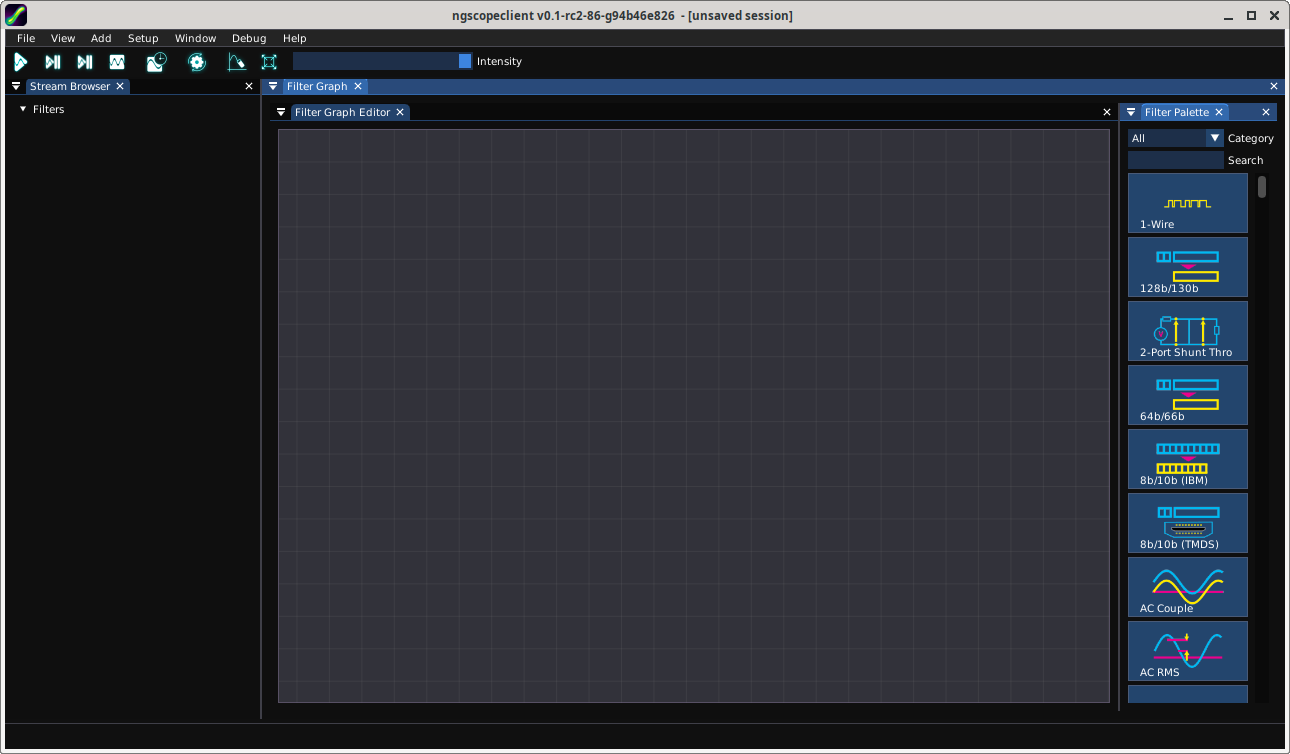
\includegraphics[width=12cm]{ng-images/empty-window.png}
\caption{Empty ngscopeclient session}
\label{empty-window}
\end{figure}

% TODO: add this section once these are implemented
\begin{comment}

\subsection{Configuration arguments}

Most of these arguments are intended for developers, but they can help troubleshoot unusual bugs.

\begin{itemize}

\item \texttt{-{}-noavx2}\\
Do not use AVX2 vector optimizations even if the CPU supports it.

\item \texttt{-{}-noavx512f}\\
Do not use AVX512F vector optimizations even if the CPU supports it.

\item \texttt{-{}-noglint64}\\
Do not use \texttt{GL\_ARB\_gpu\_shader\_int64} even if the GPU supports it.

\item \texttt{-{}-nogpufilter}\\
Do not use Vulkan (GPU accelerated) implementations of filter blocks, revert to software fallback.

\end{itemize}

\end{comment}

\subsection{Console verbosity arguments}

ngscopeclient takes standard liblogtools arguments for controlling console debug verbosity.

If no verbosity level is specified, the default is ``notice" (3). (We suggest using \texttt{-{}-debug} for routine use
until the v1.0 release to aid in troubleshooting.)

\begin{itemize}

\item \texttt{-{}-debug}\\
Sets the verbosity level to ``debug" (5).

\item \texttt{-l [file]}, \texttt{-{}-logfile [file]}\\
Writes a copy of all log messages to \texttt{file}. This is preferred over simply redirecting output with pipes, as
console escape sequences are stripped from the file log output.

\item \texttt{-L [file]}, \texttt{-{}-logfile-lines [file]}\\
Same as \texttt{-{}-logfile} except line buffering is turned on.

\item \texttt{-q}, \texttt{-{}-quiet}\\
Reduces the verbosity level by one. Can be specified more than once to lower verbosity by several steps.

\item \texttt{-{}-trace [class]}, \texttt{-{}-trace [class::function]} \\
Enables extra debug output from the class \texttt{class} or the function \texttt{class::function}. Has no effect unless
\texttt{-{}-debug} is also specified.

\item \texttt{-{}-stdout-only}\\
Sends all logging output to stdout. By default, error (level 1) and warning (level 2) messages go to stderr.

\item \texttt{-{}-verbose}\\
Sets the verbosity level to ``verbose" (4).

\end{itemize}

% TODO: add this section once these are implemented
\begin{comment}
\subsection{File arguments}
\label{import}

The file extension is used to determine the format. File extensions are case sensitive and must be lowercase to be
correctly interpreted.

\begin{itemize}
\item \texttt{[file.scopesession]}
Loads a saved session.

\item \texttt{[file.bin]} \\
Imports waveform data from the binary format used by Agilent, Keysight, and Rigol oscilloscopes.

\item \texttt{[file.complex]} \\
Imports complex I/Q data from a file. The file must contain interleaved (I, Q) pairs in either 8-bit signed/unsigned
integer, 16-bit signed integer, 32-bit normalized floating point, or 64-bit normalized floating point format.

The default format is 8 bit signed integer and may be changed from the filter graph editor or channel properties dialog
once the file is loaded. There is currently no way to specify other formats on the command line.

\item \texttt{[file.csv]} \\
Imports sample data from a CSV (comma-separated-value) file. More than one CSV file can be loaded at once (displayed as
separate points in history) by specifying multiple file names as long as they have identical column schemas.

Lines starting with a '\#' character are treated as comments and generally ignored by the parser. (If the comment format
matches that used by Digilent's WaveForms utility, timestamps and other metadata are extracted from the comments.)

If the first row of the CSV contains non-numeric characters, it is treated as a header row. Header content in the
timestamp column is ignored; headers in other columns are used as channel names in the imported waveform.

The first column of the CSV must contain sample timestamps, in seconds. Scientific notation is supported. Timestamps
must be monotonic (each row must have a timestamp strictly greater than that of the previous row).

ngscopeclient uses a heuristic to detect uniformly sampled waveforms, which enabled certain optimizations for display
and signal processing. If the standard deviation of intervals between samples is less than 1\% of the average sample
interval, the waveform is assumed to be uniformly sampled and timestamps are rounded to the nearest multiple of the
average interval. If the deviation is greater, the waveform is assumed to be sparsely sampled and timestamps are not
modified.

\item \texttt{[file.trc]} \\
Imports waveform data from a Teledyne LeCroy .trc binary waveform file.

\item \texttt{[file.vcd]} \\
Imports digital waveform data from a VCD (value change dump) file, typically created by a logic analyzer or HDL
simulator.

\item \texttt{[file.wav]} \\
Imports sample data from a WAV file.

\item \texttt{[file.wfm]} \\
Imports sample data from a Tektronix .wfm file. This import filter is still experimental and may not support all
features of the .wfm file format yet. If you have trouble importing some .wfm files please file a ticket on GitHub.

%%%%%%%%%%%%%%%%%%%%%%%%%%%%%%%%%%%%%%%%

\item \texttt{-{}-nodata}\\
When loading a .scopesession file, load settings only and not saved waveform data.

\item \texttt{-{}-reconnect}\\
When loading a .scopesession file, reconnect to the instrument and resume remote control. Current instrument settings
are overwritten with the configuration from the saved session.

\item \texttt{-{}-retrigger}\\
When loading a .scopesession file, arm the trigger immediately. has no effect unless \texttt{-{}-reconnect} is also
specified.

\end{itemize}

\subsection{Instrument arguments}

Example:
\begin{lstlisting}[language=sh, numbers=none]
./ngscopeclient --debug \
	mylecroy:lecroy:vicp:myscope.example.com:1234 \
	myrigol:rigol:lan:rigol.example.com
\end{lstlisting}

\begin{itemize}
\item \texttt{[connection string]} \\
Connects to the specified instrument. By default, all channels are enabled and displayed.

\end{itemize}

Each instrument is described by a ``connection string" containing four colon-separated fields.

\begin{itemize}
\item Nickname. This can be any text string not containing spaces or colons. If you have only one instrument it's
largely ignored, but when multiple instruments are present channel names in the UI are prefixed with the nickname to
avoid ambiguity.
\item Driver name. This is a string identifying the command protocol the scope uses. Note that not all
scopes from the same vendor will use the same command set or driver!
\item Transport. This is is a string describing how the driver connects to the scope (e.g. RS232 or Ethernet)
\item Arguments for the driver identifying the device to connect to, separated by colons. This varies by driver but is
typically a hostname:port combination, TTY device path, or similar.
\end{itemize}

\end{comment}

\include{section-tutorials}
\include{section-mainwindow}
\chapter{Dialogs}
\label{sec:dialogs}

%%%%%%%%%%%%%%%%%%%%%%%%%%%%%%%%%%%%%%%%%%%%%%%%%%%%%%%%%%%%%%%%%%%%%%%%%%%%%%%%%%%%%%%%%%%%%%%%%%%%%%%%%%%%%%%%%%%%%%%%

\section{Lab Notes}
\label{dlg:labnotes}

The Lab Notes dialog allows you to take notes on your experimental setup. It contains two tabs: ``setup notes"
and "general notes".

The contents of the Setup Notes tab are displayed on the \hyperref[dlg:speedbump]{Speed Bump} dialog when loading a
session file. The General Notes are only displayed within the Lab Notes dialog and are intended purely as a place for
recording interesting observations made during the experiment.

Minimal Markdown syntax (headings and bullets) is currently supported.\footnote{Images and links are supported by the
Markdown renderer library but the integration to properly use them is not yet finished; tables are not supported but
this will likely be added in the future.}

Lab notes are saved as Markdown files in the data directory for the session and can be opened in any
text editor or Markdown viewer. Note that they are overwritten each time the session is saved, so you should not modify
them using an external tool while the session is open in ngscopeclient or your changes may be lost.

\begin{figure}[H]
\centering
\bigimage{ng-images/dialog-labnotes.png}
\caption{Lab notes dialog}
\label{fig:labnotes}
\end{figure}

%%%%%%%%%%%%%%%%%%%%%%%%%%%%%%%%%%%%%%%%%%%%%%%%%%%%%%%%%%%%%%%%%%%%%%%%%%%%%%%%%%%%%%%%%%%%%%%%%%%%%%%%%%%%%%%%%%%%%%%%

\section{Log Viewer}
\label{dlg:logviewer}

The Log Viewer dialog provides an alternate way to view log messages sent to stdout / stderr, which may be useful for
debugging if the application was launched from a desktop icon or similar and there is no access to the console.

It can be found under the \menustyle{Window | Log Viewer} menu.

\begin{figure}[H]
\centering
\bigimage{ng-images/dialog-logviewer.png}
\caption{Log Viewer dialog}
\label{fig:logviewer}
\end{figure}

Expanding the ``settings" panel allows log messages to be filtered to show more or less detail.

Additionally, if ``trace" verbosity is selected, you can type class and/or function names using the \texttt{classname},
\texttt{classname::function}, or \texttt{::globalfunction} syntax in order to enable high-verbosity messages printed
via \texttt{LogTrace()}.

\begin{figure}[H]
\centering
\bigimage{ng-images/dialog-logviewer-trace.png}
\caption{Log Viewer dialog with tracing active}
\label{fig:logviewer-trace}
\end{figure}

%%%%%%%%%%%%%%%%%%%%%%%%%%%%%%%%%%%%%%%%%%%%%%%%%%%%%%%%%%%%%%%%%%%%%%%%%%%%%%%%%%%%%%%%%%%%%%%%%%%%%%%%%%%%%%%%%%%%%%%%

\section{Performance Metrics}
\label{dlg:perfmetrics}

The Performance Metrics dialog displays statistics on performance of rendering, waveform acquisition, and signal
processing. This data is primarily intended for developers comparing before/after performance of optimizations and code
changes.

It can be found under the \menustyle{Window | Performance Metrics} menu.

\begin{figure}[H]
\centering
\includegraphics[width=7cm]{ng-images/dialog-perfmetrics.png}
\caption{Performance Metrics dialog}
\label{fig:perfmetrics}
\end{figure}

\subsection{Rendering}

Displays render loop framerate, monitor refresh rate, total time spent last frame in the rasterization and tone
mapping shaders, and the number of vertices and indices drawn as Vulkan geometry. Note that waveforms are drawn by a
compute shader and do not contribute towards the vertex/index totals, other than a single textured rectangle used for
displaying the shader output.

\subsection{Filter graph}
Number of filter blocks in the current graph, and run time for the most recent evaluation of the
filter graph.

\subsection{Acquisition}

Displays the acquisition rate, in waveforms per second. This data is collected using a rather simple mechanism and
may not be usefully accurate if multiple trigger groups are in use.

Additionally, this section displays the number of pending waveforms for each instrument (waveforms which have been
acquired but not yet passed to the filter graph). This number should normally be flickering between zero and one if
acquisition is active and zero otherwise; larger values indicate that the instrument is supplying data faster than
ngscopeclient can process it.

\subsection{Memory}

Displays the total amount of available pinned memory (CPU-side memory eligible to be shared with the GPU) and local
memory (memory attached to the GPU), as well as the amount of each currently in use.

%%%%%%%%%%%%%%%%%%%%%%%%%%%%%%%%%%%%%%%%%%%%%%%%%%%%%%%%%%%%%%%%%%%%%%%%%%%%%%%%%%%%%%%%%%%%%%%%%%%%%%%%%%%%%%%%%%%%%%%%

\section{Preferences}
\label{dlg:preferences}

The Preferences dialog allows you to configure various application settings which are not specific to a particular
experimental setup. It can be found under the \menustyle{Setup | Preferences} menu.

\begin{figure}[H]
\centering
\includegraphics[width=7cm]{ng-images/dialog-preferences.png}
\caption{Preferences dialog}
\label{prefs}
\end{figure}

\subsection{Appearance}

This section allows you to configure fonts, colors, and other display settings for the application.

% TODO: document all of these preferences once the list has stabilized a bit

\subsection{Drivers}

This section allows you to configure default configurations for various instrument drivers.

\subsubsection{General}

\begin{itemize}
\item \emph{Headless scope default state}: When connecting to a headless oscilloscope (one without a front panel
display), specify the set of channels which should be shown after connecting.
\end{itemize}

\subsubsection{Rigol DHO}

\begin{itemize}
\item \emph{Data Width} (default auto): Specifies whether to use 8 bit or 16 bit transfer format when downloading samples
from the instrument, or automatically decide based on hardware configuration.
\end{itemize}

\subsubsection{Siglent SDS HD}

\begin{itemize}
\item \emph{Data Width} (default auto): Specifies whether to use 8 bit or 16 bit transfer format when downloading samples
from the instrument, or automatically decide based on hardware configuration.
\end{itemize}

\subsubsection{Teledyne LeCroy}

\begin{itemize}
\item \emph{Force 16 bit mode} (default on): Always use 16-bit format for downloading data from the instrument, even if
it only has an 8-bit ADC. This doubles the amount of network bandwidth required and may reduce waveforms-per-second
performance, but provides smoother waveforms.

Note that Teledyne LeCroy scopes perform DSP flatness corrections between the ADC and the data presented via the API,
meaning that even if the hardware only has an 8-bit ADC, downloading data with 16-bit precision will result in improved
accuracy.

\end{itemize}

\subsection{Files}

\begin{itemize}
\item \emph{Max recent files}: Specify the number of files to display under the \menustyle{File | Recent Files} menu.
\end{itemize}

\subsection{Miscellaneous}

\subsubsection{Menus}

\begin{itemize}
\item \emph{Recent instrument count}: Specify the number of recently used instruments to remember
\end{itemize}

\subsection{Power}

\subsubsection{Events}

This section provides settings allowing power vs performance tradeoffs. The default settings are appropriate for a
desktop or laptop running on AC power; if running on a laptop with battery power you may wish to tune these to extend
battery lifespan.

\begin{itemize}
\item \emph{Event loop mode}: Controls the operating mode for the main application event loop.
\begin{itemize}
\item In Performance mode, run at the screen refresh rate. This allows for the highest possible waveform processing rate
and the smoothest interactivity, but may waste energy if you are spending a lot of time looking at the screen without
actively acquiring or processing waveforms.
\item In Power mode, run at a greatly reduced frequency (default 4 Hz but configurable by the Polling Timeout setting)
unless a redraw is triggered by mouse movement or keyboard input. This will limit the rate of waveform acquisition and
lead to a slightly jerkier user interface, but saves power.
\end{itemize}
\item \emph{Polling timeout}: If the event loop is in Power mode, specifies the timeout before the event loop will run
if there is no user input.
\end{itemize}

%%%%%%%%%%%%%%%%%%%%%%%%%%%%%%%%%%%%%%%%%%%%%%%%%%%%%%%%%%%%%%%%%%%%%%%%%%%%%%%%%%%%%%%%%%%%%%%%%%%%%%%%%%%%%%%%%%%%%%%%

\section{Speed Bump}
\label{dlg:speedbump}

The Speed Bump dialog is displayed when loading a session file online (reconnecting to and reconfiguring hardware),
prior to committing changes to the instrument, if:

\begin{itemize}
\item The session file contains any user-created notes on the lab setup, or
\item Any of the instrument settings in the session file do not match the current configuration of the corresponding
instrument, and the direction of the change has potential to cause damage to the instrument or DUT (increasing output
voltage, removing input attenuation, etc).
\end{itemize}

This is intended as a safeguard to prevent damaging hardware by accidentally loading the wrong session file. It also
provides an opportunity to confirm that you have re-created the original experimental setup exactly if you are
switching a lab bench between multiple projects and using saved sessions to restore instrument state.

Pressing the Abort button cancels loading of the session without applying any of the potentially dangerous changes.
The instruments may be partially reconfigured in this state, as some changes (such as sample rate or memory depth
configuration) are always safe to make and thus may have been applied prior to the warning being displayed.

Pressing the Proceed button allows ngscopeclient to proceed with loading the session and reconfiguring hardware. You
must check the ``I have reviewed the instrument configuration" box in order to enable the Proceed button.

\begin{figure}[H]
\centering
\bigimage{ng-images/dialog-speedbump.png}
\caption{Speed Bump dialog}
\label{speedbump}
\end{figure}


\chapter{Workspaces and Window Management}

\section{Window Management and Docking}

All dialog boxes, waveform groups, and other GUI elements in ngscopeclient may be used docked or free-floating as
needed.

To dock a window, drag the title bar (if floating) or tab title (if docked) to the desired location (Fig.
\ref{w-docking}).

\begin{figure}[h]
\centering
\bigimage{ng-images/docking.png}
\caption{Docking a floating window}
\label{w-docking}
\end{figure}

On MacOS, Linux X11, and Windows you can drag dialogs or waveform areas out of the main ngscopeclient window to create
multiple top-level windows. This can be useful for complex experimental setups or on multi-monitor workstations.

NOTE: Multi-window mode is not currently available on Linux Wayland due to
\href{https://github.com/ocornut/imgui/issues/8609}{GUI toolkit limitations} however we hope to support this in the
future.

\section{Workspaces}

To create more complex windowing layouts, you may find it helpful to create \emph{workspaces}.

A workspace is a window which has no function of its own, and simply serves as a container for docking other windows
into. The workspace can itself be docked into another workspace or the main application window, allowing creation of
complex multi-window or multi-tab layouts to suit your experimental needs (Fig. \ref{w-workspace}, \ref{w-workspace2},
\ref{w-workspace3}).

In the default ngscopeclient window layout, for example, the "Filter Graph" tab is a workspace which contains both the
filter graph editor and the filter palette.

To rename a workspace, right click on the window title (if floating) or tab title (if docked) and enter the desired
name.

\begin{figure}[h]
\centering
\bigimage{ng-images/workspace.png}
\caption{A docked workspace containing a waveform group and two protocol analyzer tabs}
\label{w-workspace}
\end{figure}

\begin{figure}[h]
\centering
\bigimage{ng-images/workspace2.png}
\caption{Switching from the waveform workspace to the filter graph editor workspace}
\label{w-workspace2}
\end{figure}

\begin{figure}[h]
\centering
\bigimage{ng-images/workspace3.png}
\caption{Free-floating workspace not docked to the main application window}
\label{w-workspace3}
\end{figure}

\include{section-waveformgroups}
\chapter{Waveform Views}

A waveform view is a single 2D plot area within a waveform group.

Arbitrarily many channels of waveform or protocol data may be displayed within a single view, however all analog
channels within a single view share the same Y axis unit, gain, and offset. Digital channels and protocol decodes can
be overlaid on analog waveforms or displayed in their own dedicated views.

2D density plots, such as eye patterns, spectrograms, and waterfall plots, cannot share a waveform view
with any other channel.

\section{Navigation}

Scrolling with the mouse wheel adjusts the horizontal scale of the current waveform group, zooming in or out centered
on the position of the mouse cursor.

%Pressing SHIFT while scrolling moves the view left and right without adjusting zoom. If your mouse has a horizontal
%scroll feature, this may also be used to pan without zooming.

%Pressing the middle mouse button auto-scales the active waveform group so that the entire waveform is visible.

\section{Plot Area}

The plot area shows the waveform being displayed. The horizontal grid lines line up with the voltage scale markings on
the Y axis. If the plot area includes Y=0, the grid line for zero is slightly brighter.

The waveform is drawn as a semi-transparent line so that when zoomed out, the density of voltage at various points in
the graph may be seen as lighter or darker areas. This is referred to as ``intensity grading".

\begin{figure}[H]
\centering
\bigimage{ng-images/graded-waveform.png}
\caption{Intensity-graded waveform}
\label{graded-waveform2}
\end{figure}

\section{Y Axis Scale}

Each waveform view has its own Y axis scale, which is locked to the ADC range of the instrument.

Channel gain may be configured by scrolling with the mouse wheel, and offset may be adjusted by dragging the scale with
the left mouse button. Pressing the middle mouse button on the Y axis will auto-scale the vertical gain and offset to
show the full span of all channels in the view with 5\% of vertical margin.

If a left-pointing arrow (as seen in Fig. \ref{y-axis}) is visible, one of the channels in the view is selected as a
trigger source. Click on the arrow and drag up or down to select the trigger level. Some trigger types, such as window
triggers, have two arrows for upper and lower levels.

\begin{figure}[H]
\centering
\includegraphics[height=3cm]{ng-images/y-axis.png}
\caption{Waveform view showing trigger arrow on Y axis}
\label{y-axis}
\end{figure}

\section{Channel Label}

The top left corner of each waveform view contains a legend with a label for each channel being displayed in the view.

Mousing over the channel name displays a tooltip (Fig. \ref{channel-tooltip}) with some helpful information about the
waveform. The exact information displayed in the tooltip depends on the type of data being displayed, for example
analog waveforms display sample rate and record length while eye patterns display the number of integrated UIs.

\begin{figure}[H]
\centering
\includegraphics[height=3cm]{ng-images/channel-tooltip.png}
\caption{Example tooltip on channel label}
\label{channel-tooltip}
\end{figure}

The label may be dragged with the left mouse button to move the waveform to a different location. Dragging to the left
or right edge of a waveform view, or the top or bottom edge of the topmost or bottommost waveform in a group, will
split the group. Dragging to the left half of another waveform view, whether in the same group or a different group,
moves the channel to that view. Dragging to the right half of the view adds a new view within the same group containing
only the dragged waveform.

Double-clicking the label opens the channel properties dialog (Fig. \ref{channel-properties}). As with all dialogs in
ngscopeclient, the properties dialog may be left in the default floating state or docked.

\begin{figure}[H]
\centering
\includegraphics[height=5cm]{ng-images/channel-properties1.png}
\includegraphics[height=5cm]{ng-images/channel-properties2.png}
\includegraphics[height=5cm]{ng-images/channel-properties3.png}
\caption{Example of properties dialogs for three different channels}
\label{channel-properties}
\end{figure}

The properties dialog will always contain an editable nickname for the channel, a color chooser, and some basic
information about the instrument channel or filter block sourcing the data. Additional settings may be available but
will vary depending on the type of instrument or filter. In Fig. \ref{channel-properties}, the left dialog shows a
direct coaxial input to a Pico PicoScope 6824E, which has variable ADC resolution. The center dialog shows an active
differential probe with auto-zero capability, connected to a Teledyne LeCroy SDA816Zi-A which has a mux for selecting
between two input connectors for each channel. The right dialog shows a FIR filter with several configurable settings.

Right clicking on the label opens a context menu. The context menu allows setting of persistence mode, deleting the
waveform, and creating new filter blocks or protocol decodes with the selected waveform as an input.

\section{Cursors and Markers}
\label{sec:cursors}

Cursors are movable annotations which can be used to temporarily mark points of interest in a waveform and examine data
values. Markers are similar to cursors but intended for long-term marking of specific points in a single acquisition
and do not provide readout functionality.

\subsection{Vertical Cursors}

A vertical cursor describes a point in time \emph{relative to the start of the acquisition}. When new waveforms are
acquired, the cursor remains at the same offset in the new waveform. When the view is panned horizontally, the cursor
scrolls with the waveform and remains at the same point in the waveform.

To add a vertical cursor (Fig. \ref{vertical-cursor}), right click in the view and select a single or double cursor
from the \menustyle{Cursors | X Axis} menu.

Vertical cursors are attached to a waveform group and will span all views within the group. Multiple groups may have
independent vertical cursors active simultaneously.

\begin{figure}[H]
\centering
\bigimage{ng-images/vertical-cursor.png}
\caption{Single vertical cursor}
\label{vertical-cursor}
\end{figure}

\begin{figure}[H]
\centering
\bigimage{ng-images/vertical-cursor-x2.png}
\caption{Double vertical cursor}
\label{vertical-cursor-x2}
\end{figure}

To place a single cursor, click on the waveform at the desired location. To place double cursors, click at the starting
location to place the first cursor then drag to the ending location and release the mouse to place the second cursor.
Once placed, either cursor can be moved by clicking on it and dragging to the new location.

%Cursors will snap to transitions in digital signals or protocol decode overlays if the mouse is within a few pixels of
%the location. No snapping is applied when the mouse is over an analog waveform.

In the timeline each cursor will display its X-axis position. If both cursors are active, the delta between them
is shown. If the X axis uses time units, the frequency with period equal to the cursor spacing is also shown.

When a cursor is active, a dockable pop-up dialog appears displaying the value of each waveform in the group at the
cursor location. If two cursors are active, both values as well as the difference between them is shown (Fig.
\ref{vertical-cursor-x2})

%In FFT / spectrum analyzer plots, the integrated in-band power between both cursors is also shown.

\begin{comment}

If a protocol analyzer view (Chap. \ref{chapter:protoanalyzer}) is active, moving a single cursor over a packet will
scroll to and highlight that packet.

\end{comment}

\subsection{Markers}
\label{sec:markers}

A marker is a named location in \emph{absolute} time intended for marking specific events (such as protocol packets or
glitches) which may need to be re-examined in the future. When new waveforms are acquired, the marker remains attached
to the same point in the old waveform and will disappear from view until the old waveform is re-loaded from the history
window. In Fig. \ref{markers}, two of the three markers are visible while the third is in a different waveform.

Unlike vertical cursors, which are local to a single waveform group, cursors are global and will appear at the same
timestamp in all waveform groups. This allows an event of interest to be examined in detail in one view, while a
different view provides a global overview of the entire acquisition or examines another event (Fig.
\ref{marker-multiview}).

Creating a marker automatically pins the active waveform so it will not be removed from history as new data is
acquired. The waveform cannot be un-pinned unless all markers are deleted first, or the waveform itself is manually
deleted.

Newly created markers will have default numeric names such as M1, M2, etc. This name can be changed from the history
window.

\begin{figure}[H]
\centering
\bigimage{ng-images/markers.png}
\caption{Session with three markers, two on the currently displayed waveform and one on a future waveform}
\label{markers}
\end{figure}

\begin{figure}[H]
\centering
\bigimage{ng-images/marker-multiview.png}
\caption{A single marker seen at multiple time scales in different views}
\label{marker-multiview}
\end{figure}


\begin{comment}

\subsection{Horizontal Cursors}

To add a horizontal cursor (Fig. \ref{horizontal-cursor}), right click on the waveform and select \menustyle{Cursor |
Horizontal (single)} or \menustyle{Cursor | Horizontal (dual)} as appropriate.

\begin{figure}[H]
\centering
\includegraphics[width=8cm]{images/horizontal-cursor.png}
\caption{Horizontal cursor}
\label{horizontal-cursor}
\end{figure}

To place a single cursor, click on the waveform at the desired location. To place double cursors, click at the starting
location to place the first cursor then drag to the ending location and release the mouse to place the second cursor.
Once placed, either cursor can be moved by clicking on it and dragging to the new location.

At the right side of the plot, each cursor will display its Y-axis location. If both cursors are active, the delta
between them is also shown.

All waveform areas in a group share the same Y axis cursor positions.
\end{comment}

\chapter{History}
\label{sec:history}

ngscopeclient saves a rolling buffer of previous waveforms in memory, allowing you to go back in time and see previous
state of the system being debugged. This buffer is included in saved sessions, allowing a full snapshot of system
behavior to be loaded for future analysis. History is always captured up to the configured depth, regardless of whether
the history view window is displayed or not.

Clicking on a timestamp in the history view (Fig. \ref{historyview}) pauses acquisition and loads the historical
waveform data for analysis.

\begin{figure}[H]
\centering
\includegraphics[width=7cm]{ng-images/history.png}
\caption{Waveform history view}
\label{historyview}
\end{figure}

Hovering the mouse over a row in the history view (Fig. \ref{history-tooltip}) displays a tooltip with the full date
and time of the acquisition, as well as some information about which instruments and channels had data in the capture
(if some channels were enabled or disabled during the lab session, the set of active channels may have changed
throughout history).

\begin{figure}[H]
\centering
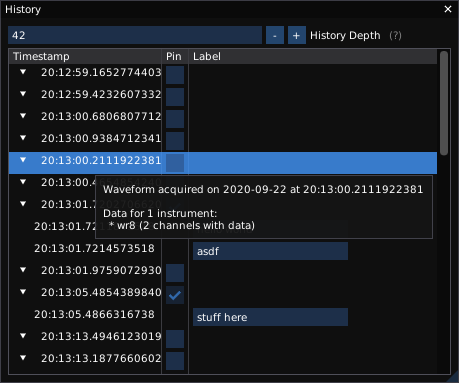
\includegraphics[width=7cm]{ng-images/history-tooltip.png}
\caption{Tooltip on waveform history entry}
\label{history-tooltip}
\end{figure}

The history depth defaults to 10 waveforms, but can be set arbitrarily within the limits of available RAM. All history
must fit in system RAM in the current software version; spilling to disk is planned for the future
(\issue{scopehal-apps}{311}). Older waveforms beyond the history limit are deleted automatically as new waveforms are
acquired. Any single waveform in history may also be deleted by right clicking on the line and selecting ``delete" from
the menu.

%The status bar at the bottom of the history view displays the total number of waveforms in the history, as well as an
%estimate of the amount of RAM used by the history.

\section{Pinning}

Interesting waveforms may be ``pinned" in the history by checking the box in the ``pin" column of the history view.
Pinned waveforms are retained in the history buffer even when new waveforms arrive; only unpinned waveforms
are eligible for automatic deletion to make space for incoming data.

If a waveform contains markers (\ref{sec:markers}), it is automatically pinned and cannot be unpinned unless the marker
(or entire waveform) is manually deleted. This prevents accidental loss of an important waveform: if the event was
important enough to mark and name, it is probably worth keeping around.

\section{Labeling}

Arbitrary text names may be assigned to a waveform by clicking the corresponding cell in the ``label" column. As with
waveforms containing markers, waveforms with a label are automatically pinned since assigning a label implies the
waveform is important.

\begin{comment}

\section{Estimating Waveform Memory Usage}

When selecting a maximum depth for the history, it is important to pick a reasonable limit to avoid running out of RAM!
ngscopeclient will happily fill tens or hundreds of gigabytes of memory with deep waveforms if given a chance. Memory
usage of waveform data can be roughly estimated as 16 + sizeof(sample type) bytes per point, since each sample contains a
64-bit timestamp and duration plus the sample data.

For example, an analog sample takes 20 bytes of RAM (16 of time plus a 32-bit floating point voltage measurement) per
sample. Thus, a 1M point analog waveform takes approximately 20 MB of RAM per channel, or 80 MB per capture on a
four-channel oscilloscope with all channels enabled.

On the larger side, a 10M point four channel capture would use 800 MB and a 64M point deep-memory capture would use 5
GB. A deep history setting, such as 100 waveforms, is thus wildly inappropriate for such deep captures! A future
software release may support spilling waveform data to a temporary directory on disk, permitting effectively unlimited
history depth given sufficient disk space.

Digital waveforms use one byte per sample for the actual measurement, so 17 MB per channel for a 1M point waveform.
Most logic analyzer or MSO drivers for libscopehal will perform automatic de-duplication when a waveform goes several
clock cycles with no toggles, so the actual memory usage is likely to be significantly less than this.

Filter memory usage varies depending on the specific filter in question, however it is typically not a large
contributor to the overall ngscopeclient RAM footprint when using history mode because filters are evaluated
dynamically each time a waveform is pulled from history rather than having output cached for every historical waveform.
Thus, at most one copy of each filter's output is present in memory regardless of history depth.
\end{comment}

\chapter{Stream Browser}
\label{streambrowser}

\section{Introduction}

The stream browser is the primary navigation pane for quick access to instrument settings and channels. By default in a
new ngscopeclient session it is docked to the left side of the window but it can be repositioned as needed.

\begin{figure}[H]
\centering
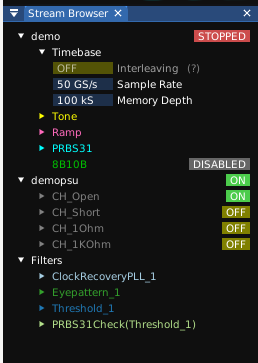
\includegraphics[width=7cm]{ng-images/streambrowser.png}
\caption{Example configuration of the stream browser}
\label{streambrowser}
\end{figure}

NOTE: The stream browser is one of the more recent additions to ngscopeclient and is undergoing rapid development. Some
changes to appearance and interaction metaphors should be expected in upcoming versions as we unify the user interface
to be more consistent for all types of instrument.

\section{Filters}

The "filters" node contains a list of all filter graph blocks active in the current session. Expanding the node for a
given filter will show a list of output streams.

\section{Instruments}

The node for each instrument contains a list of all channels on the instrument, whether enabled or not. Depending on
the type of instrument, additional nodes with commonly used settings such as timebase configuration may be available.

Color coded ``badges" are displayed in the right margin next to channels or instruments in some cases, displaying
context-dependent information such as trigger state, power supply or signal generator on/off status, etc. These badges
are clickable to change the relevant setting.

\section{Adding streams}

Instrument channels, filters, and streams can be dragged from the browser to other parts of ngscopeclient in order to
visualize or interact with data from them. For example:

\begin{itemize}
\item Drag a scalar stream to the measurements window to display its real-time value
\item Drag a currently-inactive channel to the filter graph view to add a node for the channel so it can be used
\item Drag a stream to a waveform area to display it in that plot
\end{itemize}

\chapter{Filter Graph Editor}
\label{grapheditor}

\section{Introduction}

The filter graph editor allows complex signal processing pipelines to be developed in a graphical fashion and is the
first window created automatically in a new session. It may be reopened from the \menustyle{Window | Filter Graph} menu
item if closed.

The graph editor view (Fig. \ref{graph-editor}) shows nodes for every instrument channel, trigger, and filter block
used in the current session. Additional nodes for inactive channels may be created by dragging them from the stream
browser into the graph editor canvas.

Nodes cannot overlap and will automatically move out of the way if
another node is dragged on top of them.

\begin{figure}[H]
\centering
\bigimage{ng-images/graph-editor.png}
\caption{Filter graph editor showing instrument channels and several processing blocks}
\label{graph-editor}
\end{figure}

\section{Interaction}

The view may be zoomed with the mouse wheel, or panned by dragging with the right mouse button, to navigate large
filter graphs which do not fit on a single screen at a reasonable zoom level. Right clicking on a node opens a pop-up
properties view (Fig. \ref{graph-editor-properties}).

\begin{figure}[H]
\centering
\includegraphics[width=8cm]{ng-images/graph-editor-properties.png}
\caption{Filter graph editor showing properties popup}
\label{graph-editor-properties}
\end{figure}

Nodes display inputs at left and outputs at right. To connect two existing nodes, click on an input or output port and
drag to the port you wish to connect it to. An input can only connect to one output at a time; if the destination
already is connected to a different signal the previous connection will be removed and replaced with the new one.

A tooltip with a green plus sign is displayed during dragging if the proposed connection is valid. If the tooltip
displays a red X instead, the connection is invalid (connecting two inputs, two outputs, or an input and output of
incompatible data types).

To create a new node, click on an input or output port and drag to an empty area of the canvas (Fig.
\ref{graph-editor-create}, Fig. \ref{graph-editor-addinput}). A context menu will appear, presenting a list of filters
which can accept (if dragging from an output) or produce (if dragging from an input) the desired data type. If dragging
from an input, the context menu will also include any currently unused instrument channels.

\begin{figure}[H]
\centering
\bigimage{ng-images/graph-editor-create.png}
\caption{Filter graph editor dragging from an output to an empty area of the canvas}
\label{graph-editor-create}
\end{figure}

\begin{figure}[H]
\centering
\includegraphics[width=10cm]{ng-images/graph-editor-addinput.png}
\caption{Filter graph editor dragging from an input to an empty area of the canvas}
\label{graph-editor-addinput}
\end{figure}

When a new node is added to the filter graph, each output channel will be automatically added to an existing waveform
view if a compatible one is present. If no compatible view is available, a new view and/or group will be created.

Node title bars are color-coded to match the display color of the waveform trace, allowing easy navigation between
waveform views and the graph editor.

Each node also includes a caption stating the type of node (``hardware input", ``hardware output", or the name of the
filter block) and, in most cases, an icon depicting the functionality of the block.\footnote{Not all filters currently
have icons. We are working with multiple artists to create more filter icons and welcome additional contributions.}

\section{Grouping}

In order to better organize complex experimental setups, nodes may be organized in groups. Groups cannot be nested.

To create a group, right click an unused area of the graph editor canvas and select ``New Group" from the context menu.
This will spawn a new, empty group near the mouse cursor position.

The group will have an automatically generated name (Fig. \ref{graph-editor-group1}) by default. This name may be
changed by right clicking on the group's title bar and typing a new name in the pop-up.

\begin{figure}[H]
\centering
\bigimage{ng-images/graph-editor-group1.png}
\caption{Newly created node group}
\label{graph-editor-group1}
\end{figure}

To add a node to a group, simply drag the node by its title bar and move it into the group (Fig.
\ref{graph-editor-group2}). All paths from the node to the remainder of the filter graph will be routed through
``hierarchical ports" at the left and right edges of the group, reducing clutter. Nodes may be freely moved around
within the group to organize them, or dragged out of the group to remove them from the group.

A group (together with its contents) may be moved by dragging the group's title bar with the left mouse button, or
resized by dragging any of its corners. When a group is moved, it will push other nodes or groups out of the way to
prevent overlapping.

If not needed, a group can be deleted by selecting it with the left mouse button and pressing the ``delete" key.
Deleting a group does not remove any nodes contained within it.

\begin{figure}[H]
\centering
\bigimage{ng-images/graph-editor-group2.png}
\caption{Groups containing several nodes with hierarchical ports}
\label{graph-editor-group2}
\end{figure}

\chapter{Transports}
\label{sec:transports}

Libscopehal uses a ``transport" object in order to pass commands and data to instruments, in order to decouple the
specifics of LXI, USBTMC, etc. from individual instrument drivers. This section describes the supported transports and
their usage and limitations.

Not all transports are possible to use with any given driver due to hardware limitations or software/firmware quirks.
For details on which transport(s) are usable with a particular instrument, consult the documentation for that device's
driver.

\section{gpib}

SCPI over GPIB.

This transport takes up to four arguments: GPIB board index, primary address, secondary address, and timeout value.
Only board index and primary address are required. We currently support using a single GPIB device per GPIB board
(interface) in a ngscopeclient session. You cannot currently access multiple devices in the same or across instances.
Better support for multiple instrument on a single board is planned.

NOTE: The current implementation of this driver only works on Linux, using the linux-gpib library. Since linux-gpib is licensed under GNU GPL, this driver is packaged separately and must be installed from \url{https://github.com/ngscopeclient/scopehal-plugins-gpl}.

Example:
\begin{lstlisting}[language=sh, numbers=none]
ngscopeclient myscope:keysightdca:gpib:0:7
\end{lstlisting}

\section{lan}

SCPI over TCP with no further encapsulation.

This transport takes two arguments: hostname/IP and port number.

If port number is not specified, uses TCP port 5025 (IANA assigned) by default. Note that Rigol oscilloscopes use the
non-standard port 5555, not 5025, so the port number must always be specified when using a Rigol instrument.

Example:
\begin{lstlisting}[language=sh, numbers=none]
ngscopeclient myscope:rigol:lan:192.0.2.9:5555
\end{lstlisting}

\section{lxi}

SCPI over LXI VXI-11.

Note that due to the remote procedure call paradigm used by LXI, it is not possible to batch multiple outstanding
requests to an instrument when using this transport. Some instruments may experience reduced performance when using LXI
as the transport. Drivers which require command batching may not be able to use LXI VXI-11 as the transport even if the
instrument supports it.

Example:
\begin{lstlisting}[language=sh, numbers=none]
ngscopeclient myscope:tektronix:lxi:192.0.2.9
\end{lstlisting}

\section{null}

This transport does nothing, and is used as a placeholder for development simulations or non-SCPI instruments.

NOTE: Due to limitations of the current command line argument parsing code, an argument must be provided to all
transports, including this one, when connecting via the command line. Since the argument is ignored, any non-empty
string may be used.

Example:
\begin{lstlisting}[language=sh, numbers=none]
ngscopeclient sim:demo:null:blah
\end{lstlisting}

\section{socketcan}

This transport provides a bridge for accessing the native Linux SocketCAN API from the scopehal driver layer. When
paired with the ``socketcan" oscilloscope driver and a suitable CAN peripheral, it allows ngscopeclient to be used as a
CAN bus protocol analyzer. Since SocketCAN is a Linux-only API, this transport is not available on other platforms.

This transport takes one argument: the device name (e.g. ``can0")

\section{twinlan}

This transport is used by some Antikernel Labs oscilloscopes, as well as most of the bridge servers used for interfacing
libscopehal with USB oscilloscopes' SDKs. It takes three arguments: hostname/IP and two port numbers.

It uses two TCP sockets on different ports. The first carries SCPI text (as in the ``lan" transport), and the second is
for binary waveform data.

If port numbers are not specified, the SCPI port defaults to the IANA standard of 5025, and the data port defaults to
5026. If the SCPI port but not the data port is specified, the data port defaults to the SCPI port plus one.

\section{uart}

SCPI over RS-232 or USB-UART.

This transport takes 3 arguments: device path (required), baud rate (optional), and flags (optional). If baud rate is not specified, it
defaults to 115200.

Example:
\begin{lstlisting}[language=sh, numbers=none]
ngscopeclient myscope:rigol:uart:/dev/ttyUSB0:115200
\end{lstlisting}

Some devices, like the NanoVNA, need to activate the DTR line to communicate. This can be achieved by adding the DTR flag to the connection string.

Example:
\begin{lstlisting}[language=sh, numbers=none]
ngscopeclient NanoVNA-F:nanovna:uart:COM6:115200:DTR
\end{lstlisting}


\section{usbtmc}

SCPI over USB Test \& Measurement Class protocol.

This transport takes two arguments: the path to the usbtmc kernel device object and the TMC transfer size (optional). As Workaround for Siglent SDS1x04x-E set size to 48.

NOTE: The current implementation of this driver only works on Linux. There is currently no support for USBTMC on
Windows (\issue{scopehal}{301})

Example:
\begin{lstlisting}[language=sh, numbers=none]
ngscopeclient myscope:siglent:usbtmc:/dev/usbtmc0:48
\end{lstlisting}

\section{vicp}

SCPI over Teledyne LeCroy Virtual Instrument Control Protocol.

This transport takes two arguments: hostname/IP and port number.

If port number is not specified, uses TCP port 1861 (IANA assigned) by default.

Example:
\begin{lstlisting}[language=sh, numbers=none]
ngscopeclient myscope:lecroy:vicp:192.0.2.9
\end{lstlisting}

\section{hid}

This transport layer is usually used by binary drivers to communicate with Test \& Measurement equiment over USB.

This transport takes two arguments: vendor ID (hex) and product ID (hex).

Optionally a third argument can be added with the instrument's serial number.
If not provided, the instrument's serial number is automatically pulled at first connection and stored in the connection string.

Example:
\begin{lstlisting}[language=sh, numbers=none]
ngscopeclient AlientekDP100:alientek_dp:hid:2e3c:af01
\end{lstlisting}

\include{section-bert-drivers}
\include{section-funcgen-drivers}
\include{section-load-drivers}
\include{section-meter-drivers}
\include{section-misc-drivers}
\chapter{Oscilloscope Drivers}
\label{sec:scope-drivers}

This chapter describes all of the available drivers for oscilloscopes and logic analyzers.

\section{Agilent}

Agilent devices support a similar similar SCPI command set across most device families.

Please see the table below for details of current hardware support:

\begin{tabularx}{16cm}{lllX}
\thickhline
\textbf{Device Family} & \textbf{Driver} & \textbf{Transport} & \textbf{Notes} \\
\thickhline
DSO5000 series & agilent & lan & Not recently tested, but should work.\\
\thinhline
DSO6000 \& MSO6000 series & agilent & lan &  Working. No support for digital channels yet.\\
\thinhline
DSO7000 \& MSO7000 series & agilent & lan & Untested, but should work. No support for digital channels yet.\\
\thinhline
EDUX1000 series & agilent & lan & Untested but should be identical to DSOX1200 but with lower sample memory. \\
\thinhline
DSOX1200 series & agilent & lan & Working. No support for wavegen yet. \\
\thinhline
MSOX-2000 series & agilent & lan \\
\thinhline
MSOX-3000 series & agilent & lan \\
\thickhline
\end{tabularx}

\subsection{agilent}

\subsubsection{Typical Performance (MSO6034A, LAN)}

Interestingly, performance sometimes gets better with more channels or deeper memory. Not sure why.

\begin{tabularx}{16cm}{llX}
\thickhline
\textbf{Channels} & \textbf{Memory depth} & \textbf{WFM/s}\\
\thickhline
1 & 1K & 66 \\
\thinhline
4 & 1K & 33 \\
\thinhline
4 & 4K & 33 \\
\thinhline
1 & 40K & 33 \\
\thinhline
1 & 4K & 22 \\
\thinhline
1 & 20K & 22 \\
\thinhline
4 & 20K & 22 \\
\thinhline
1 & 100K & 22 \\
\thinhline
4 & 10K & 17 \\
\thinhline
4 & 40K & 12 \\
\thinhline
1 & 200K & 11 \\
\thinhline
1 & 400K & 8 \\
\thinhline
4 & 100K & 6.5 \\
\thinhline
4 & 200K & 4 \\
\thinhline
1 & 1M & 3.7 \\
\thinhline
4 & 400K & 2.3 \\
\thinhline
1 & 1M & 1 \\
\thinhline
4 & 1M & 1 \\
\thinhline
4 & 4M & 0.2 \\
\thickhline
\end{tabularx}

\subsubsection{Typical Performance (MSOX3104T, LAN)}

\begin{tabularx}{16cm}{llX}
\thickhline
\textbf{Channels} & \textbf{Memory depth} & \textbf{WFM/s}\\
\thickhline
1 & 2.5K & 3.3 \\
\thinhline
4 & 2.5K & 2.5 \\
\thinhline
1 & 2.5M & 1.0 \\
\thinhline
4 & 2.0M & 0.5 \\
\thickhline
\end{tabularx}

\section{Antikernel Labs}

\begin{tabularx}{16cm}{llX}
\thickhline
\textbf{Device Family} & \textbf{Driver} & \textbf{Notes} \\
\thickhline
Internal Logic Analyzer IP & akila & \\
\thickhline
BLONDEL Oscilloscope Prototype & aklabs & \\
\thickhline
\end{tabularx}

\subsection{akila}

This driver uses a raw binary protocol, not SCPI.

Under-development internal logic analyzer analyzer core for FPGA design debug. The ILA uses a UART interface to a host
system. Since there's no UART support in scopehal yet, socat must be used to bridge the UART to a TCP socket using
the ``lan" transport.

\subsection{aklabs}

This driver uses two TCP sockets. Port 5025 is used for SCPI control plane traffic, and port 50101 is used for waveform
data using a raw binary protocol.

\section{Demo}

The ``demo" driver is a simulation-only driver for development and training purposes, and does not connect to real
hardware.

It ignores any transport provided, and is normally used with the ``null" transport.

The demo instrument is intended to illustrate the usage of ngscopeclient for various types of analysis and to aid in
automated testing on computers which do not have a connection to a real oscilloscope, and is not intended to accurately
model the response or characteristics of real world scope frontends or signals.

It supports memory depths of 10K, 100K, 1M, and 10M points per waveform at rates of 1, 5, 10, 25, 50, and 100 Gsps.
Four test signals are provided, each with 10 mV of Gaussian noise and a 5 GHz low-pass filter added (although this can
be disabled under the channel properties)

Test signals:
\begin{itemize}
\item 1.000 GHz tone
\item 1.000 GHz tone mixed with a second tone, which sweeps from 1.100 to 1.500 GHz
\item 10.3125 Gbps PRBS-31
\item 1.25 Gbps repeating two 8B/10B symbols (K28.5 D16.2)
\end{itemize}

\begin{tabularx}{16cm}{lllX}
\thickhline
\textbf{Device Family} & \textbf{Driver} & \textbf{Transport} & \textbf{Notes} \\
\thickhline
Simulator & demo & null & \\
\thickhline
\end{tabularx}

\section{Digilent}

Digilent oscilloscopes using the WaveForms SDK are all supported using the ``digilent" driver in libscopehal. This
driver connects using the ``twinlan" transport to a \href{https://github.com/ngscopeclient/scopehal-waveforms-bridge}
{socket server} which links against the Digilent WaveForms SDK. This provides network transparency, and allows the
Digilent bridge server to be packaged separately for distribution and only installed by users who require it.

As of 2022-03-09, analog input channels on the Analog Discovery Pro and Analog Discovery 2 have been tested and are
functional, however only basic edge triggering is implemented so far. Analog inputs on other devices likely work,
however only these two have been tested to date.

Analog outputs, digital inputs, and digital outputs are currently unimplemented, but are planned to be added in the
future.

\subsection{digilent}

\begin{tabularx}{16cm}{lllX}
\thickhline
\textbf{Device Family} & \textbf{Driver} & \textbf{Transport} & \textbf{Notes} \\
\thickhline
Electronics Explorer & digilent & twinlan & Not tested, but probably works\\
\thinhline
Analog Discovery & digilent & twinlan & Not tested, but probably works\\
\thinhline
Analog Discovery 2 & digilent & twinlan & No digital channel support \newline No analog output support\\
\thinhline
Analog Discovery Pro & digilent & twinlan & No digital channel support \newline No analog output support \\
\thinhline
Digital Discovery & digilent & twinlan & No digital channel support,\newline so pretty useless for now\\
\thickhline
\end{tabularx}

\subsubsection{Typical Performance (ADP3450, USB -> LAN)}

\begin{tabularx}{16cm}{llX}
\thickhline
\textbf{Channels} & \textbf{Memory depth} & \textbf{WFM/s}\\
\thickhline
4 & 64K & 25.8 \\
\thinhline
2 & 64K & 32.3 \\
\thinhline
1 & 64K & 33.0 \\
\thickhline
\end{tabularx}

\section{DrAndyHaas}

\subsection{haasoscope pro}

HaasoscopePro is an affordable 2 GHz bandwidth 3.2 GS/s (expandable to 6.4 GS/s) 12-bit open-source open-hardware USB oscilloscope.
For more info see the \href{https://github.com/drandyhaas/HaasoscopePro}{HaasoscopePro github}.
This driver connects to a Haasoscope Pro GUI, which must first be running, over a LAN socket.
It supports ~50 Hz of update rate for moderate memory depth.

\begin{tabularx}{16cm}{llX}
\thickhline
\textbf{Device Family} & \textbf{Driver} & \textbf{Notes} \\
\thickhline
DrAndyHaas & haasoscope pro & lan on port 32001 \\
\thickhline
\end{tabularx}

\section{DreamSource Lab}

DreamSourceLabs oscilloscopes and logic analyzers supported in their fork of sigrok (``libsigrok4DSL'' distributed as part of
their ``DSView'' software package) are supported through the ``dslabs'' driver in libscopehal. This driver connects using
the ``twinlan'' transport to a \href{https://github.com/ngscopeclient/scopehal-sigrok-bridge}{socket server} which links
against libsigrok4DSL. This provides network transparency, and allows the DSLabs bridge server to be packaged separately for
distribution and only installed by users who require it.

As of 2022-03-22, a DSCope U3P100 and a DSLogic U3Pro16has been tested and works adequately. Other products may work
also, but are untested.

On DSCope: Only edge triggers are supported. `Any' edge is not supported. ``Ch0 \&\& Ch1'' and ``Ch0 || Ch1'' trigger modes
are not supported.

On DSLogic: Only edge triggers are supported. All edges are supported. There is currently no way to configure a trigger on more
than one channel. Serial / multi-stage triggers are not supported.

Known issues pending fixes/refactoring:
\begin{itemize}
	\item Interleaved sample rates are not correctly reported in the timebase dialog (but are in the waveform display)
	\item Trigger position is quantized to multiples of 1\% of total capture
	\item Non-localhost performance, and responsiveness in general may suffer as a result of hacky flow control on waveform capture
	\item DSLogic depth configuration is confusing and performance could be improved (currently only buffered more is supported)
	\item DSLogic devices trigger even if pre-trigger buffer has not been filled, leading to a small pre-trigger waveform in some cases
\end{itemize}

\subsection{dslabs}

\begin{tabularx}{16cm}{lllX}
\thickhline
\textbf{Family / Device} & \textbf{Driver} & \textbf{Transport} & \textbf{Notes} \\
\thickhline
DScope U3P100 & dslabs & twinlan & Tested, works\\
\thinhline
DSLogic U3P16 & dslabs & twinlan & Tested, works\\
\thinhline
DSCope (others) & dslabs & twinlan & Not tested, but probably works\\
\thinhline
DSLogic (others) & dslabs & twinlan & Not tested, but probably works\\
\thickhline
\end{tabularx}

\subsubsection{Typical DSCope Performance (DSCope U3P100, USB3, localhost)}

\begin{tabularx}{16cm}{lllXX}
\thickhline
\textbf{Channels} & \textbf{Memory depth} & \textbf{Sample Rate} & \textbf{WFM/s} & \textbf{UI-unconstrained WFM/s}\\
\thickhline
2 & 1M & 100MS/s & 14 & 50\\
\thinhline
2 & 5M & 500MS/s & 4.5 & 14\\
\thinhline
1 & 5M & 1GS/s & 8.3 & 32\\
\thickhline
\end{tabularx}

\subsubsection{Typical DSLogic Performance (DSLogic U3Pro16, USB3, localhost)}

\begin{tabularx}{16cm}{lllXX}
\thickhline
\textbf{Channels} & \textbf{Memory depth} & \textbf{Sample Rate} & \textbf{WFM/s} & \textbf{UI-unconstrained WFM/s}\\
\thickhline
16 & 500k & 100MS/s & 16 & 44\\
\thinhline
16 & 500k & 500MS/s & 16 & 55\\
\thickhline
\end{tabularx}

\section{EEVengers}

\subsection{thunderscope}

This driver connects to the TS.NET application to control a ThunderScope.

It supports full-rate 1 Gsps streaming given suitably fast hardware.

\begin{tabularx}{16cm}{llX}
\thickhline
\textbf{Device Family} & \textbf{Driver} & \textbf{Notes} \\
\thickhline
ThunderScope & thunderscope & Use twinlan transport to TS.NET \\
\thickhline
\end{tabularx}

\section{Enjoy Digital}
TODO (\issue{scopehal}{79})

\section{Generic}

Drivers in this section are not specific to a particular manufacturer's products and support a wide variety of similar
devices.

\subsection{socketcan}

This driver exposes the Linux SocketCAN API as a stream of CAN messages which can be displayed as-is or used as input
to other filter graph blocks. When paired with the ``socketcan" transport and a suitable CAN peripheral, it allows
ngscopeclient to be used as a CAN bus protocol analyzer. Since SocketCAN is a Linux-only API, this driver is not
available on other platforms.

\section{Hantek}
TODO (\issue{scopehal}{26})

\section{Keysight}

Keysight devices support a similar similar SCPI command set across most device families. Many Keysight devices were
previously sold under the Agilent brand and use the same SCPI command set, so they are supported by the ``agilent"
driver.

Please see the table below for details of current hardware support:

\subsection{agilent}

\begin{tabularx}{16cm}{llX}
\thickhline
\textbf{Device Family} & \textbf{Driver} & \textbf{Notes} \\
\thickhline
MSOX-2000 series & agilent &  \\
\thinhline
MSOX-3000 series & agilent &  \\
\thinhline
MSOX-3000T series & agilent &  \\
\thickhline
\end{tabularx}

\subsection{keysightdca}

A driver for the Keysight/Agilent/HP DCA series of equivalent-time sampling oscilloscopes.

\begin{tabularx}{16cm}{llX}
\thickhline
\textbf{Device Family} & \textbf{Driver} & \textbf{Notes} \\
\thickhline
86100A & keysightdca &  \\
\thickhline
\end{tabularx}

\section{Pico Technologies}

Pico oscilloscopes all have slightly different command sets, but are supported using the ``pico" driver in libscopehal.
This driver connects via a TCP socket to a socket server
\href{https://github.com/ngscopeclient/scopehal-pico-bridge}{scopehal-pico-bridge} which connects to the appropriate
instrument using Pico's binary SDK.

\begin{tabularx}{16cm}{llX}
\thickhline
\textbf{Device Family} & \textbf{Driver} & \textbf{Notes} \\
\thickhline
3000D series & pico & Early development, incomplete\\
\thinhline
6000E series & pico & \\
\thickhline
\end{tabularx}

\subsection{pico}

\subsubsection{Typical Performance (6824E, LAN)}

\begin{tabularx}{16cm}{llX}
\thickhline
\textbf{Channels} & \textbf{Memory depth} & \textbf{WFM/s}\\
\thickhline
8 & 1M & 15.2 \\
\thinhline
4 & 1M & 30.5 \\
\thinhline
2 & 1M & 64.4 \\
\thinhline
1 & 10M & 12.2 \\
\thinhline
1 & 50M & 3.03 \\
\thickhline
\end{tabularx}

\section{Rigol}

Rigol oscilloscopes have subtle differences in SCPI command set, but this is implemented with quirks handling in the
driver rather than needing different drivers for each scope family.

NOTE: DS1054Z firmware 00.04.02.SP4 is known to have problems with SCPI remote control
(https://github.com/ngscopeclient/scopehal-apps/issues/790); it is unclear what other models and firmware versions may
be affected by this bug. If you encounter problems, please ensure your scope is running the latest firmware release
from Rigol before opening a support ticket.

\begin{tabularx}{16cm}{llX}
\thickhline
\textbf{Device Family} & \textbf{Driver} & \textbf{Notes} \\
\thickhline
DS1100D/E & rigol & \\
\thinhline
DS1000Z & rigol & \\
\thinhline
MSO5000 & rigol & \\
\thinhline
DHO800 & rigol & \\
\thinhline
DHO900 & rigol & (no digital channels)\\
\thinhline
DHO1000 & rigol & (untested)\\
\thinhline
DHO4000 & rigol & (untested)\\
\thickhline
\end{tabularx}

\subsection{rigol}

\subsubsection{Typical Performance (MSO5000 series, LAN)}

\begin{tabularx}{16cm}{llX}
\thickhline
\textbf{Channels} & \textbf{Memory depth} & \textbf{WFM/s}\\
\thickhline
4 & 10K & 0.96 \\
\thinhline
4 & 100K & 0.91 \\
\thinhline
4 & 1M & 0.59\\
\thinhline
4 & 10M & 0.13\\
\thinhline
1 & 100M & 0.0601\\
\thinhline
4 & 25M & 0.0568\\
\thinhline
2 & 50M & 0.0568\\
\thickhline
\end{tabularx}

\subsubsection{Typical Performance (DHO800/900 series, LAN)}

\begin{tabularx}{16cm}{llX}
\thickhline
\textbf{Channels} & \textbf{Memory depth} & \textbf{WFM/s}\\
\thickhline
1 & 1K & 11.9 (live mode available for 1Kpt/single channel)\\
\thinhline
2 & 1K & 3.4 \\
\thinhline
4 & 1K & 1.66 \\
\thinhline
1 & 10K & 3.31 \\
\thinhline
2 & 10K & 2.90 \\
\thinhline
4 & 10K & 1.65 \\
\thinhline
1 & 100K & 3.30 \\
\thinhline
4 & 100K & 1.64 \\
\thinhline
1 & 1M & 1.63 \\
\thinhline
4 & 1M & 0.57 \\
\thinhline
1 & 10M & 0.30 \\
\thinhline
4 & 10M & 0.07 \\
\thickhline
\end{tabularx}

\section{Rohde \& Schwarz}

\subsection{rs}

There is partial support for RTM3000 (and possibly others, untested) however it appears to have bitrotted.

TODO (\issue{scopehal}{59})

\subsection{rs\_rto6}

This driver supports the newer RTO6 family scopes (and possibly others, untested).

\section{Saleae}
TODO (\issue{scopehal}{16})

\section{Siglent}

A driver for SDS2000X+/HD is available in the codebase which has been developed according to Siglent offical documentation
(Programming Guide PG01-E11A). This driver should be functional across the 'next generation' SDS800X HD, SDS1000X HD, SDS2000X+,
SDS2000X HD, SDS5000X, SDS6000A/L/Pro and SDS7000A scopes. It has been primarily developed using the SDS2000X+ and SDS2000X HD.
Some older generation scopes are supported as well.

Digital channels are not supported on any scope yet, due to lack of an MSO probe to test with. Many trigger types are
not yet supported.

\begin{tabularx}{16cm}{lllX}
\thickhline
\textbf{Device Family} & \textbf{Driver} & \textbf{Transport} & \textbf{Notes} \\
\thickhline
SDS1000X-E series & siglent & lan & Initialises, triggers and downloads waveforms. More testing needed \\
\thinhline
SDS2000X-E series & siglent & lan & Initialises, triggers and downloads waveforms. More testing needed \\
\thickhline
SDS800X HD series & siglent & lan & Basic functionality complete/tested. \\
\thinhline
SDS1000X HD series & siglent & lan & Basic functionality complete, needs testing. \\
\thinhline
SDS2000X+ series & siglent & lan & Basic functionality complete. \\
\thinhline
SDS2000X HD series & siglent & lan & Tested and works well on SDS2354x HD. \\
\thinhline
SDS3000X HD series & siglent & lan & Basic functionality complete, needs testing. \\
\thinhline
SDS5000X series & siglent & lan & Initialises, triggers and downloads waveforms. More testing needed \\
\thinhline
SDS6000A/L/Pro series & siglent & lan & Tested and works well on SDS6204A. 10/12 bit models NOT supported, but unavailable for dev (not sold in western markets). \\
\thinhline
SDS7000A series & siglent & lan & Basic functionality complete, needs testing. \\
\thickhline
\end{tabularx}

\subsubsection{Typical Performance (SDS2104X+, LAN)}

\begin{figure}[h]
\centering
\includegraphics[width=16cm]{images/siglent-samples.png}
\caption{Siglent sample speed for various combinations of depth and channels}
\label{siglent_sample}
\end{figure}


\begin{tabularx}{16cm}{llX}
\thickhline
\textbf{Channels} & \textbf{Memory depth} & \textbf{WFM/s}\\
\thickhline
1 & 5-100K & 2.3 \\
\thinhline
2 & 5-100K & 1.6 \\
\thinhline
3 & 5-100K & 1.2 \\
\thinhline
4 & 5-100K & 1 \\
\thinhline
1 & 10M & 0.5 \\
\thinhline
2-4 & 10M & 0.15 \\
\thickhline
\end{tabularx}

These figures were obtained from a SDS2104X+ running firmware version 1.3.7R5. Different scopes and software
revisions may vary.

\subsubsection{Typical Performance (SDS2104X HD, LAN)}

\begin{tabularx}{16cm}{llX}
\thickhline
\textbf{Channels} & \textbf{Memory depth} & \textbf{WFM/s}\\
\thickhline
1 & 10K & 8.2 \\
\thinhline
2 & 10K & 7.7 \\
\thinhline
4 & 10K & 5.4 \\
\thinhline
1 & 100K & 7.1 \\
\thinhline
4 & 100K & 4.2 \\
\thinhline
1 & 5M & 0.72 \\
\thinhline
4 & 5M & 0.09 \\
\thickhline
\end{tabularx}

These figures were obtained from a SDS2104X HD running firmware version 1.2.2.9.

\section{Teledyne LeCroy / LeCroy}

Teledyne LeCroy (and older LeCroy) devices use the same driver, but two different transports for LAN connections.

While all Teledyne LeCroy / LeCroy devices use almost identical SCPI command sets, Windows based devices running
XStream or MAUI use a custom framing protocol (``vicp") around the SCPI data while the lower end RTOS based devices use
raw SCPI over TCP (``lan").

Please see the table below for details on which configuration to use with  your hardware.

\begin{tabularx}{16cm}{lllX}
\thickhline
\textbf{Device Family} & \textbf{Driver} & \textbf{Transport} & \textbf{Notes} \\
\thickhline
DDA & lecroy & vicp & Tested on DDA5000A series \\
\thinhline
HDO & lecroy & vicp & Tested on HDO9000 series \\
\thinhline
LabMaster & lecroy & vicp & Untested, but should work for 4-channel setups\\
\thinhline
MDA & lecroy & vicp & Untested, but should work\\
\thinhline
SDA & lecroy & vicp & Tested on SDA 8Zi and 8Zi-A series\\
\thinhline
T3DSO & ??? & ??? & Untested\\
\thinhline
WaveAce & ??? & ??? & Untested\\
\thinhline
WaveJet & ??? & ??? & Untested\\
\thinhline
WaveMaster & lecroy & vicp & Same hardware as SDA/DDA\\
\thinhline
WaveRunner & lecroy & vicp & Tested on WaveRunner Xi, 8000, and 9000 series\\
\thinhline
WaveSurfer & lecroy & vicp & Tested on WaveSurfer 3000 series \\
\thickhline
\end{tabularx}

\subsection{lecroy}

This is the primary driver for MAUI based Teledyne LeCroy / LeCroy devices.

This driver has been tested on a wide range of Teledyne LeCroy / LeCroy hardware. It should be compatible with any
Teledyne LeCroy or LeCroy oscilloscope running Windows XP or newer and the MAUI or XStream software.

\subsubsection{Typical Performance (HDO9204, VICP)}

\begin{tabularx}{16cm}{llX}
\thickhline
\textbf{Channels} & \textbf{Memory depth} & \textbf{WFM/s}\\
\thickhline
1 & 100K & >50 \\
\thinhline
1 & 400K & 29 - 35 \\
\thinhline
2 & 100K & 30 - 40 \\
\thinhline
4 & 100K & 17 - 21 \\
\thinhline
1 & 2M & 9 - 11 \\
\thinhline
1 & 10M & 2.2 - 2.6 \\
\thinhline
4 & 1M & 5.2 - 6.5 \\
\thinhline
1 & 64M & 0.41 - 0.42 \\
\thinhline
2 & 64M & 0.21 - 0.23 \\
\thinhline
4 & 64M & 0.12 - 0.13 \\
\thickhline
\end{tabularx}

\subsubsection{Typical Performance (WaveRunner 8404M-MS, VICP)}

\begin{tabularx}{16cm}{llX}
\thickhline
\textbf{Channels} & \textbf{Memory depth} & \textbf{WFM/s}\\
\thickhline
1 & 80K & 35 - 45 \\
\thinhline
2 & 80K & 35 - 45 \\
\thinhline
2 & 800K & 16 - 17 \\
\thinhline
2 & 8M & 3.1 - 3.2 \\
\thickhline
\end{tabularx}

\subsection{lecroy\_fwp}

This is a special performance-enhanced extension of the base ``lecroy" driver which takes advantage of the FastWavePort
feature of the instrument to gain high speed access to waveform data via shared memory. Waveforms are pulled from
shared memory when a synchronization event fires, then pushed to the client via a separate TCP socket on port 1862.

On low latency LANs, typical performance increases observed with SDA 8Zi series instruments are on the order of 2x
throughput vs using the base driver downloading waveforms via SCPI. On higher latency connections such as VPNs, the
performance increase is likely to be even higher because the push-based model eliminates the need for polling (which
performs increasingly poorly as latency increases).

To use this driver, your instrument must have the XDEV software option installed and the
\href{https://github.com/ngscopeclient/scopehal-fwp-bridge}{scopehal-fwp-bridge} server application running. If the
bridge or option are not detected, the driver falls back to SCPI waveform download and will behave identically to the
base ``lecroy" driver.

There are some limitations to be aware of with this driver:
\begin{itemize}

\item Maxmimum memory depth is limited to no more than 40M samples per channel, regardless of installed instrument
memory. This is an architectural limitation of the FastWavePort API; the next generation FastMultiWavePort API eliminates
this restriction however scopehal-fwp-bridge does not yet support it due to poor documentation.

\item MSO channels are not supported, because neither FastWavePort nor FastMultiWavePort provide shared memory access to
digital channel data. There is no known workaround for this given current instrument APIs.

\item A maximum of four analog channels are supported even if the instrument actually has eight. There are no major
technical blockers to fixing this under FastWavePort however no 8-channel instruments are available to the developers as
of this writing, so there is no way to test potential fixes. FastMultiWavePort has a limit of four channels per instance,
but it may be possible to instantiate multiple copies of the FastMultiWavePort block to work around this.

\item Math functions F9-F12 are used by the FastWavePort blocks and cannot be used for other math functions.

\end{itemize}

\section{Tektronix}

This driver is being primarily developed on a MSO64. It supports SCPI over LXI VXI-11 or TCP sockets.

The hardware supports USBTMC, however waveform download via USBTMC does not work with libscopehal for unknown reasons.

\begin{tabularx}{16cm}{lllX}
\thickhline
\textbf{Device Family} & \textbf{Driver} & \textbf{Transport} & \textbf{Notes} \\
\thickhline
MSO5 series & tektronix & lan, lxi &  \\
\thinhline
MSO6 series & tektronix & lan, lxi &  \\
\thickhline
\end{tabularx}

\subsection{Note regarding ``lan" transport on MSO5/6}

The default settings for raw SCPI access on the MSO6 series use a full terminal emulator rather than raw SCPI
commands. To remove the prompts and help text, go to Utility | I/O, then under the Socket Server panel select protocol
``None" rather than the default of ``Terminal".

\subsubsection{Typical Performance (MSO64, LXI, embedded OS)}

\begin{tabularx}{16cm}{llX}
\thickhline
\textbf{Channels} & \textbf{Memory depth} & \textbf{WFM/s}\\
\thickhline
1 & 50K & 10.3 - 11.4 \\
\thinhline
2 & 50K & 6.7 - 7.2 \\
\thinhline
4 & 50K & 5.1 - 5.3 \\
\thinhline
1 & 500K & 8.7 - 9.5 \\
\thinhline
4 & 500K & 3.8 - 3.9 \\
\thickhline
\end{tabularx}

\section{tinySA}

This driver is meant to be used with tinySA and tinySA ULTRA spectrum analyzers.

It has been developed and tested on a tinySA ULTRA.

The communication with the device is made with UART transport layer.

\begin{tabularx}{16cm}{lllX}
\thickhline
\textbf{Device Family} & \textbf{Driver} & \textbf{Transport} & \textbf{Notes} \\
\thickhline
tinySA  & tiny\_sa & uart & Not tested but should work \\
\thinhline
tinySA ULTRA & tiny\_sa & uart & Driver tested on this device \\
\thickhline
\end{tabularx}

\section{Xilinx}
TODO (\issue{scopehal}{40})

\include{section-sdr-drivers}
\chapter{Spectrometer Drivers}
\label{sec:spec-drivers}

This chapter describes all of the available drivers for optical (UV/VIS/IR) spectrometers.

\section{ASEQ Instruments}

\begin{tabularx}{16cm}{lllX}
\thickhline
\textbf{Device Family} & \textbf{Driver} & \textbf{Transport} & \textbf{Notes} \\
\thickhline
LR1 & aseq & twinlan & Use \href{https://github.com/ngscopeclient/scopehal-aseq-bridge}{scopehal-aseq-bridge}\\
\thickhline
\end{tabularx}

\subsection{aseq}

This driver supports the ASEQ Instruments LR1 spectrometer (and possibly others, not tested) via an external bridge
server and the ASEQ USB control API.

\chapter{Power Supply Drivers}
\label{sec:powersupply-drivers}

This chapter describes all of the available drivers for power supplies.

% TODO: demo driver

\section{Alientek}

\begin{tabularx}{16cm}{lllX}
\thickhline
\textbf{Device Family} & \textbf{Driver} & \textbf{Transport} & \textbf{Notes} \\
\thickhline
DP100 & alientek\_dp & hid & \\
\thickhline
\end{tabularx}

\subsection{alientek\_dp}

This driver works on Alientek DP100 mini Digital Power Supply.

Path for connection (vendorId:productId) is: 2e3c:af01.

\section{GW Instek}

\begin{tabularx}{16cm}{lllX}
\thickhline
\textbf{Device Family} & \textbf{Driver} & \textbf{Transport} & \textbf{Notes} \\
\thickhline
GPD-X303S series & gwinstek\_gpdx303s & uart & 9600 Baud default. Tested with GPD-3303S. No support for tracking modes yet.\\
\thickhline
\end{tabularx}

\subsection{gwinstek\_gpdx303s}

Supported models should include GPD-2303S, GPD-3303S, GPD-4303S, and GPD-3303D.

\section{Kuaiqu}

\begin{tabularx}{16cm}{lllX}
\thickhline
\textbf{Device Family} & \textbf{Driver} & \textbf{Transport} & \textbf{Notes} \\
\thickhline
Kuaiqu SSPS-S series & kuaiqu\_psu & uart & \\
Kuaiqu SPPS*D series & kuaiqu\_psu & uart & \\
Kuaiqu SPPS-D series & kuaiqu\_psu & uart & Tested on a Kuaiqu SPPS-D3010-232\\
Kuaiqu R-SPPS series & kuaiqu\_psu & uart & \\
\thickhline
\end{tabularx}

\subsection{kuaiqu\_psu}

This driver supports all Kuaiqu programmable PSUs, including SSPS-S, SPPS*D, SPPS-D and R-SPPS series.

It has been tested on a Kuaiqu SPPS-D3010-232.

\section{Riden}

\begin{tabularx}{16cm}{lllX}
\thickhline
\textbf{Device Family} & \textbf{Driver} & \textbf{Transport} & \textbf{Notes} \\
\thickhline
Riden RD series & riden\_rd & uart & Tested on a Riden RD6006\\
\thickhline
\end{tabularx}

\subsection{kuaiqu\_psu}

This driver supports all Riden RD series DC Power Supplies.

It has been tested on a Riden RD6006.

\section{Rigol}

\begin{tabularx}{16cm}{lllX}
\thickhline
\textbf{Device Family} & \textbf{Driver} & \textbf{Transport} & \textbf{Notes} \\
\thickhline
DP832, DP832A & rigol\_dp8xx & uart, usbtmc, lan & No support for tracking modes yet.\\
\thickhline
\end{tabularx}

\subsection{rigol\_dp8xx}

This driver supports the DP832 and DP832A.

\section{Rohde \& Schwarz}

\begin{tabularx}{16cm}{lllX}
\thickhline
\textbf{Device Family} & \textbf{Driver} & \textbf{Transport} & \textbf{Notes} \\
\thickhline
HMC804x series & rs\_hmc804x & uart, usbtmc, lan & No support for tracking modes yet.\\
\thickhline
\end{tabularx}

\subsection{rs\_hmc804x}

This driver should support the HMC8041, HMC8042, and HMC8043 but has only been tested on the HMC8042.

\section{Siglent}

\begin{tabularx}{16cm}{lllX}
\thickhline
\textbf{Device Family} & \textbf{Driver} & \textbf{Transport} & \textbf{Notes} \\
\thickhline
SPD3303X series & siglent\_spd & lan & Tested with SPD3303X-E\\
\thickhline
\end{tabularx}

\subsection{siglent\_spd}

Supported models should include SPD3303X, SPD3303X-E.

NOTE: Channel 3 of the SPD3303x series does not support software voltage/current adjustment. It has a fixed current
limit of 3.2A, and output voltage selectable to 2.5, 3.3, or 5V via a mechanical switch. While channel 3 can be turned
on and off under software control, there is no readback capability whatsoever for channel 3 in the SCPI API.

As a result - regardless of actual hardware state - the driver will report channel 3 as being in constant voltage mode.
Additionally, the driver will report channel 3 as being off until it is turned on by software. Once the output has been
turned on, the driver will track the state and report a correct on/off state as long as no front panel control buttons
are touched.

\section{Sinilink}

\begin{tabularx}{16cm}{lllX}
\thickhline
\textbf{Device Family} & \textbf{Driver} & \textbf{Transport} & \textbf{Notes} \\
\thickhline
XY series & siniLink & uart & Tested on a XYS3580\\
\thickhline
\end{tabularx}

\subsection{siniLink}

This driver should be compatible with most Sinilink XY series powersupplies.
The driver might also work with Sinilink sk series powersupplies.

\include{section-rfgen-drivers}
\include{section-vna-drivers}
\chapter{Triggers}

\section{Trigger Properties}

The \menustyle{Setup / Trigger} menu opens the trigger properties dialog (Fig. \ref{trigger-properties}).

The Type dropdown allows the type of trigger to be chosen. The list of available triggers depends on the instrument
model and installed software options.

The Position field specifies the time from the \emph{start} of the waveform to the trigger point. Positive values
move the trigger later into the waveform, negative values introduce a delay between the trigger and the start of the
waveform. \footnote{This is a different convention than most oscilloscopes, which typically measure the trigger
position from the \emph{midpoint} of the waveform. Since ngscopeclient decouples the acquisition length from the UI
zoom setting, measuring from the midpoint makes little sense as there are no obvious visual cues to the midpoint's
location.}

\begin{figure}[h]
\centering
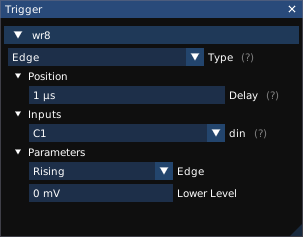
\includegraphics[width=7cm]{ng-images/trigger-properties.png}
\caption{Trigger properties dialog}
\label{trigger-properties}
\end{figure}

The remaining settings in the trigger properties dialog depend on the specific trigger type chosen.

\section{Serial Pattern Triggers}

All serial pattern triggers take one or two pattern fields, a radix, and a condition.

For conditions like ``between" or ``not between" both patterns are used, and no wildcards are allowed. For other
conditions, only the first pattern is used.

Patterns may be specified as ASCII text, hex, or binary. ``Don't care" nibbles/bits may be specified in hex/binary
patterns as ``X", for example ``3fx8" or ``1100010xxx1".

\pagebreak

%%%%%%%%%%%%%%%%%%%%%%%%%%%%%%%%%%%%%%%%%%%%%%%%%%%%%%%%%%%%%%%%%%%%%%%%%%%%%%%%%%%%%%%%%%%%%%%%%%%%%%%%%%%%%%%%%%%%%%%%
\section{Dropout}

Triggers when a signal stops toggling for a specified amount of time.

\subsection{Inputs}

\begin{tabularx}{16cm}{llX}
\thickhline
\textbf{Signal name} & \textbf{Type} & \textbf{Description} \\
\thickhline
din & Analog or digital & Input signal \\
\end{tabularx}

\subsection{Parameters}

\begin{tabularx}{16cm}{llX}
\thickhline
\textbf{Parameter name} & \textbf{Type} & \textbf{Description} \\
\thickhline
Edge & Enum & Specifies the polarity of edge to look for (rising or falling) \\
\thinhline
Dropout Time & Int & Dropout time needed to trigger \\
\thinhline
Level & Float & Voltage threshold\\
\thinhline
Reset Mode & Enum & Specifies whether to reset the timer on the opposite edge \\
\thickhline
\end{tabularx}

%%%%%%%%%%%%%%%%%%%%%%%%%%%%%%%%%%%%%%%%%%%%%%%%%%%%%%%%%%%%%%%%%%%%%%%%%%%%%%%%%%%%%%%%%%%%%%%%%%%%%%%%%%%%%%%%%%%%%%%%
\section{Edge}

Triggers on edges in the signal.

Edge types ``rising" and ``falling" are self-explanatory. ``Any" triggers on either rising or falling edges.
``Alternating" is a unique trigger mode only found on certain Agilent/Keysight oscilloscopes, which alternates each
waveform between rising and falling edge triggers.

\subsection{Inputs}

\begin{tabularx}{16cm}{llX}
\thickhline
\textbf{Signal name} & \textbf{Type} & \textbf{Description} \\
\thickhline
din & Analog or digital & Input signal \\
\end{tabularx}

\subsection{Parameters}

\begin{tabularx}{16cm}{llX}
\thickhline
\textbf{Parameter name} & \textbf{Type} & \textbf{Description} \\
\thickhline
Edge & Enum & Specifies the polarity of edge to look for\\
\thinhline
Level & Float & Voltage threshold\\
\thickhline
\end{tabularx}

%%%%%%%%%%%%%%%%%%%%%%%%%%%%%%%%%%%%%%%%%%%%%%%%%%%%%%%%%%%%%%%%%%%%%%%%%%%%%%%%%%%%%%%%%%%%%%%%%%%%%%%%%%%%%%%%%%%%%%%%
\section{Glitch}

TODO: This is supported on at least LeCroy hardware, but it's not clear how it differs from pulse width.

%%%%%%%%%%%%%%%%%%%%%%%%%%%%%%%%%%%%%%%%%%%%%%%%%%%%%%%%%%%%%%%%%%%%%%%%%%%%%%%%%%%%%%%%%%%%%%%%%%%%%%%%%%%%%%%%%%%%%%%%

\section{Pulse Width}

Triggers when a high or low pulse meeting specified width criteria is seen.

\begin{tabularx}{16cm}{llX}
\thickhline
\textbf{Signal name} & \textbf{Type} & \textbf{Description} \\
\thickhline
din & Analog or digital & Input signal \\
\thickhline
\end{tabularx}

\subsection{Parameters}

\begin{tabularx}{16cm}{llX}
\thickhline
\textbf{Parameter name} & \textbf{Type} & \textbf{Description} \\
\thickhline
Condition & Enum & Match condition (greater, less, between, or not between) \\
\thinhline
Edge & Enum & Specifies the polarity of edge to look for\\
\thinhline
Level & Float & Voltage threshold\\
\thinhline
Lower Bound & Int & Lower width threshold\\
\thinhline
Upper Bound & Int & Upper width threshold\\
\thickhline
\end{tabularx}

%%%%%%%%%%%%%%%%%%%%%%%%%%%%%%%%%%%%%%%%%%%%%%%%%%%%%%%%%%%%%%%%%%%%%%%%%%%%%%%%%%%%%%%%%%%%%%%%%%%%%%%%%%%%%%%%%%%%%%%%
\section{Runt}

Triggers when a pulse of specified width crosses one threshold, but not a second.

\begin{tabularx}{16cm}{llX}
\thickhline
\textbf{Signal name} & \textbf{Type} & \textbf{Description} \\
\thickhline
din & Analog & Input signal \\
\thickhline
\end{tabularx}

\subsection{Parameters}

\begin{tabularx}{16cm}{llX}
\thickhline
\textbf{Parameter name} & \textbf{Type} & \textbf{Description} \\
\thickhline
Condition & Enum & Match condition (greater, less, between, or not between) \\
\thinhline
Edge Slope & Enum & Specifies the polarity of edge to look for\\
\thinhline
Lower Interval & Int & Lower width threshold\\
\thinhline
Lower Level & Float & Lower voltage threshold\\
\thinhline
Upper Interval & Int & Upper width threshold\\
\thinhline
Upper Level & Float & Upper voltage threshold\\
\thickhline
\end{tabularx}

%%%%%%%%%%%%%%%%%%%%%%%%%%%%%%%%%%%%%%%%%%%%%%%%%%%%%%%%%%%%%%%%%%%%%%%%%%%%%%%%%%%%%%%%%%%%%%%%%%%%%%%%%%%%%%%%%%%%%%%%
\section{Slew Rate}

Triggers when an edge is faster or slower than a specified rate.

\begin{tabularx}{16cm}{llX}
\thickhline
\textbf{Signal name} & \textbf{Type} & \textbf{Description} \\
\thickhline
din & Analog & Input signal \\
\thickhline
\end{tabularx}

\subsection{Parameters}

\begin{tabularx}{16cm}{llX}
\thickhline
\textbf{Parameter name} & \textbf{Type} & \textbf{Description} \\
\thickhline
Condition & Enum & Match condition (greater, less, between, or not between) \\
\thinhline
Edge Slope & Enum & Specifies the polarity of edge to look for\\
\thinhline
Lower Interval & Int & Lower width threshold\\
\thinhline
Lower Level & Float & Lower voltage threshold\\
\thinhline
Upper Interval & Int & Upper width threshold\\
\thinhline
Upper Level & Float & Upper voltage threshold\\
\thickhline
\end{tabularx}

%%%%%%%%%%%%%%%%%%%%%%%%%%%%%%%%%%%%%%%%%%%%%%%%%%%%%%%%%%%%%%%%%%%%%%%%%%%%%%%%%%%%%%%%%%%%%%%%%%%%%%%%%%%%%%%%%%%%%%%%
\section{UART}

Triggers when a byte or byte sequence is seen on a UART.

\subsection{Inputs}

\begin{tabularx}{16cm}{llX}
\thickhline
\textbf{Signal name} & \textbf{Type} & \textbf{Description} \\
\thickhline
din & Analog or digital & Input signal \\
\thickhline
\end{tabularx}

\subsection{Parameters}

\begin{tabularx}{16cm}{llX}
\thickhline
\textbf{Parameter name} & \textbf{Type} & \textbf{Description} \\
\thickhline
Bit Rate & Int & Baud rate \\
\thinhline
Condition & Enum & Match condition \\
\thinhline
Level & Float & Voltage threshold\\
\thinhline
Parity Mode & Enum & Odd, even, or no parity \\
\thinhline
Pattern & String & First match pattern\\
\thinhline
Pattern 2 & String & Second match pattern \\
\thinhline
Polarity & Enum & Idle high (normal UART) or idle low (RS232)\\
\thinhline
Radix & Enum & Radix for the patterns\\
\thinhline
Stop Bits & Float & Number of stop bits\\
\thinhline
Trigger Type & Enum & Match data pattern or parity error\\
\thickhline
\end{tabularx}

%%%%%%%%%%%%%%%%%%%%%%%%%%%%%%%%%%%%%%%%%%%%%%%%%%%%%%%%%%%%%%%%%%%%%%%%%%%%%%%%%%%%%%%%%%%%%%%%%%%%%%%%%%%%%%%%%%%%%%%%

\section{Window}

Triggers when a signal goes above or below specified thresholds.

The available configuration settings for this trigger vary from instrument to instrument.

\begin{tabularx}{16cm}{llX}
\thickhline
\textbf{Signal name} & \textbf{Type} & \textbf{Description} \\
\thickhline
din & Analog & Input signal \\
\thickhline
\end{tabularx}

\subsection{Parameters}

\begin{tabularx}{16cm}{llX}
\thickhline
\textbf{Parameter name} & \textbf{Type} & \textbf{Description} \\
\thickhline
Condition & Enum & Specifies whether to trigger on entry or exit from the window, and whether to trigger immediately or
after a time limit.\\
\thinhline
Edge & Enum & Specifies which edge of the window to trigger on\\
\thinhline
Lower Level & Float & Lower voltage threshold\\
\thinhline
Upper Level & Float & Upper voltage threshold\\
\thickhline
\end{tabularx}


\chapter{Filters}

\section{Introduction}

\subsection{Key Concepts}

ngscopeclient and libscopehal are based on a ``filter graph" architecture internally. The filter graph is a directed
acyclic graph with a set of source nodes (waveforms captured from hardware, loaded from a saved session, or generated
numerically) and sink nodes (waveform views, protocol analyzer views, and statistics) connected by edges representing
data flow.

A filter is simply an intermediate node in the graph, which takes input from zero or more waveform nodes and outputs a
waveform which may be displayed, used as input to other filters, or both. A waveform is a series of data points which
may represent voltages, digital samples, or arbitrarily complex protocol data structures.

As a result, there is no internal distinction between math functions, measurements, and protocol decodes, and it is
possible to chain them arbitrarily. Consider the following example:

\begin{itemize}
\item Two analog waveforms representing serial data and clock are acquired
\item Each analog waveform is thresholded, producing a digital waveform
\item The two digital waveforms are decoded as $I^2C$, producing a series of packets
\item The $I^2C$ packets are decoded as writes to a serial DAC, producing an analog waveform
\item A moving average filter is applied to the analog waveform
\item A measurement filter finds the instantaneous frequency of each cycle of the DAC output
\end{itemize}

In this document we use the term ``filter" consistently to avoid ambiguity.

\subsection{Conventions}

A filter can take arbitrarily many inputs (vector or scalar values from the filter graph), arbitrarily many parameters
(static scalar configuration settings), and outputs arbitrarily many vector or scalar outputs.

If the output signal is a multi-field type (as opposed to a single scalar, e.g. voltage, at each sample) the
``Output Signal" section will include a table describing how various types of output data are displayed.

All filters with complex output use a standardized set of colors to display various types of data fields in a
consistent manner. These colors are configurable under the \menustyle{Appearance / Decodes} preferences category.

\begin{tabularx}{16cm}{llX}
\thickhline
\textbf{Color name} & \textbf{Use case} & \textbf{Default Color} \\
\thickhline
Address & Memory addresses & \cellcolor{address}\textcolor{black}{\#ffff00} \\
\thinhline
Checksum Bad & Incorrect CRC/checksum & \cellcolor{checksumbad}\textcolor{white}{\#ff0000} \\
\thinhline
Checksum OK & Valid CRC/checksum & \cellcolor{checksumok}\textcolor{black}{\#00ff00} \\
\thinhline
Control & Miscellaneous control data & \cellcolor{control}\textcolor{white}{\#c000a0} \\
\thinhline
Data & User data & \cellcolor{data}\textcolor{white}{\#336699} \\
\thinhline
Error & Malformed/unreadable data & \cellcolor{error}\textcolor{white}{\#ff0000} \\
\thinhline
Idle & Inter-frame gaps & \cellcolor{idle}\textcolor{white}{\#404040} \\
\thinhline
Preamble & Preamble/sync words & \cellcolor{preamble}\textcolor{white}{\#808080} \\
\thickhline
\end{tabularx}

%%%%%%%%%%%%%%%%%%%%%%%%%%%%%%%%%%%%%%%%%%%%%%%%%%%%%%%%%%%%%%%%%%%%%%%%%%%%%%%%%%%%%%%%%%%%%%%%%%%%%%%%%%%%%%%%%%%%%%%%
\pagebreak
\section{128b/130b}
\label{filter:128b130b}

Decodes the 128b/130b line code used by PCIe gen 3/4/5. This filter performs block alignment and descrambling, but no
decoding of block contents.

128b/130b, as a close relative of \hyperref[filter:128b130b]{64b/66b}, is a serial line code which divides transmitted
data into 128-bit blocks and scrambles them with a LFSR, then appends a 2-bit type field (which is not scrambled) to
each block for synchronization. Block synchronization depends on always having an edge in the type field so types 2'b00
and 2'b11 are disallowed.

For PCIe over 128b/130b, block type 2'b01 contains 128 bits of upper layer protocol data while block type 2'b10
contains an ordered set.

Note that this filter only performs block alignment and descrambling. No decoding or parsing is applied to the 128-bit
blocks, other than searching for skip ordered sets (beginning with 0xaa) and using them for scrambler synchronization.

\begin{figure}[h]
\centering
\bigimage{ng-images/filters/128b130b.png}
\caption{Example 128b/130b decode}
\label{filter_128b130b}
\end{figure}

\begin{figure}[h]
\centering
\bigimage{ng-images/filters/graph-pcie-gen3.png}
\caption{Example filter graph using 128b/130b to decode a 2-lane PCIe gen3 link}
\label{filter_graph_128b130b}
\end{figure}

\subsection{Inputs}

\begin{tabularx}{16cm}{llX}
\thickhline
\textbf{Signal name} & \textbf{Type} & \textbf{Description} \\
\thickhline
data & Digital & Serial 128b/130b data line \\
\thinhline
clk & Digital & DDR bit clock, typically generated by use of the \hyperref[filter:cdrpll]{Clock Recovery
(PLL)} filter on the input data.\\
\thickhline
\end{tabularx}

\subsection{Parameters}

This filter takes no parameters.

\subsection{Output Signal}

The 128B/130B filter outputs a time series of 128B/130B sample objects. These consist of a control/data flag and
a 128-bit data block.

\begin{tabularx}{16cm}{llX}
\thickhline
\textbf{Stream name} & \textbf{Type} & \textbf{Description} \\
\thickhline
data & Sparse protocol & Output decode \\
\thickhline
\end{tabularx}

\begin{tabularx}{16cm}{lllX}
\thickhline
\textbf{Type} & \textbf{Description} & \textbf{Color} & \textbf{Format} \\
\thickhline
Ordered set & Block with type 2'b10 & \cellcolor{control}\textcolor{white}{Control} & \%032x \\
\thinhline
Data & Block with type 2'b01 & \cellcolor{data}\textcolor{white}{Data} & \%032x \\
\thinhline
Error & Block with type 2'b00 or 2'b11 & \cellcolor{error}\textcolor{white}{Error} & \%032x \\
\thickhline
\end{tabularx}

%%%%%%%%%%%%%%%%%%%%%%%%%%%%%%%%%%%%%%%%%%%%%%%%%%%%%%%%%%%%%%%%%%%%%%%%%%%%%%%%%%%%%%%%%%%%%%%%%%%%%%%%%%%%%%%%%%%%%%%%
\pagebreak
\section{2-Port Shunt Through}
\label{filter:2portshuntthrough}

Measures the impedance of a DUT connected to a VNA in a 2-port shunt-through topology (VNA ports 1 and 2 connected,
with DUT attached between the connection point and ground). This is commonly used for measuring very low impedance
networks, such as power distribution networks.

(This filter description is a stub and will be expanded in the future)

%%%%%%%%%%%%%%%%%%%%%%%%%%%%%%%%%%%%%%%%%%%%%%%%%%%%%%%%%%%%%%%%%%%%%%%%%%%%%%%%%%%%%%%%%%%%%%%%%%%%%%%%%%%%%%%%%%%%%%%%
\pagebreak
\section{64b/66b}
\label{filter:64b66b}

Decodes the 64/66b line code used by \hyperref[filter:10gbaser]{10Gbase-R} and other serial protocols, as originally
specified in IEEE 802.3 clause 49.2.

64b/66b is a serial line code which divides transmitted data into 64-bit blocks and scrambles them with a LFSR, then
appends a 2-bit type field (which is not scrambled) to each block for synchronization. Block synchronization depends on
always having an edge in the type field so types 2'b00 and 2'b11 are disallowed.

Note that this filter only performs block alignment and descrambling. No decoding is applied to the 64-bit blocks, as
different upper-layer protocols assign different meaning to them. In 10Gbase-R, type 2'b01 denotes ``64 bits of upper
layer data" and type 2'b10 denotes ``8-bit type field and 56 bits of data whose meaning depends on the type", however
this is not universal and some other protocols use these fields for different purposes.

\begin{figure}[h]
\centering
\bigimage{ng-images/filters/64b66b.png}
\caption{Example 64b/66b decode}
\label{filter_64b66b}
\end{figure}

\begin{figure}[h]
\centering
\bigimage{ng-images/filters/graph-10gbe.png}
\caption{Example filter graph using 64b/66b to decode a 10Gbase-R signal}
\label{filter_graph_64b66b}
\end{figure}

\subsection{Inputs}

\begin{tabularx}{16cm}{llX}
\thickhline
\textbf{Signal name} & \textbf{Type} & \textbf{Description} \\
\thickhline
data & Digital & Serial 64b/66b data line \\
\thinhline
clk & Digital & DDR bit clock, typically generated by use of the \hyperref[filter:cdrpll]{Clock Recovery
(PLL)} filter on the input data.\\
\thickhline
\end{tabularx}

\subsection{Parameters}

This filter takes no parameters.

\subsection{Output Signal}

The 64B/66B filter outputs a time series of 64B/66B sample objects. These consist of a control/data flag and
a 64-bit data block.

\begin{tabularx}{16cm}{llX}
\thickhline
\textbf{Stream name} & \textbf{Type} & \textbf{Description} \\
\thickhline
data & Sparse protocol & Output decode \\
\thickhline
\end{tabularx}

\begin{tabularx}{16cm}{lllX}
\thickhline
\textbf{Type} & \textbf{Description} & \textbf{Color} & \textbf{Format} \\
\thickhline
Control & Block with type 2'b10 & \cellcolor{control}\textcolor{white}{Control} & \%016x \\
\thinhline
Data & Block with type 2'b01 & \cellcolor{data}\textcolor{white}{Data} & \%016x \\
\thinhline
Error & Block with type 2'b00 or 2'b11 & \cellcolor{error}\textcolor{white}{Error} & \%016x \\
\thickhline
\end{tabularx}

%%%%%%%%%%%%%%%%%%%%%%%%%%%%%%%%%%%%%%%%%%%%%%%%%%%%%%%%%%%%%%%%%%%%%%%%%%%%%%%%%%%%%%%%%%%%%%%%%%%%%%%%%%%%%%%%%%%%%%%%
\pagebreak
\section{8B/10B (IBM)}
\label{filter:8b10b}

Decodes the standard 8b/10b line code used by \hyperref[filter:sgmii]{SGMII}, \hyperref[filter:1000basex]{1000base-X},
DisplayPort, JESD204A/B, \hyperref[filter:pcie2_logical]{PCIe gen 1/2}, SATA, USB 3.0, and many other common serial
protocols.

8b/10b is a dictionary based code which converts each byte of message data to a ten-bit code. In order to maintain DC
balance and limit run length to a maximum of five identical bits in a row, all 8-bit input codes have one of:
\begin{itemize}
\item One legal coding, with exactly five zero bits
\item Two legal codings, one with four zero bits and one with six
\end{itemize}

The transmitter maintains a ``running disparity" counter and chooses the appropriate coding for each symbol to ensure
DC balance. There are twelve legal codes which are not needed for encoding data values; these are used to encode
frame boundaries, idle/alignment sequences, and other control information.

\begin{figure}[h]
\centering
\bigimage{ng-images/filters/8b10b.png}
\caption{Example 8b/10b decode}
\label{filter_8b10b}
\end{figure}

\begin{figure}[h]
\centering
\bigimage{ng-images/filters/graph-1000basex.png}
\caption{Example filter graph using 8b/10b to decode a differential 1000base-X link}
\label{filter_graph_8b10b}
\end{figure}

\subsection{Inputs}

\begin{tabularx}{16cm}{llX}
\thickhline
\textbf{Signal name} & \textbf{Type} & \textbf{Description} \\
\thickhline
data & Digital & Serial 8b/10b data line \\
\thinhline
clk & Digital & DDR bit clock, typically generated by use of the \hyperref[filter:cdrpll]{Clock Recovery
(PLL)} filter on the input data.\\
\thickhline
\end{tabularx}

\subsection{Parameters}

\begin{tabularx}{16cm}{llX}
\thickhline
\textbf{Parameter name} & \textbf{Type} & \textbf{Description} \\
\thinhline
Comma Search Window & Integer &
Number of unit intervals to search when performing comma alignment. A larger window increases the probability of a
correct lock if commas are infrequent, but significantly slows down the decode. The default is 20000 UI. \\
\thinhline
Display Format & Enum &
	\textbf{Dotted (K28.5 D21.5)}: displays the 3b4b and 5b6b code blocks separately, with K or D prefix, as well as the current running disparity. \newline
	\textbf{Hex (K.bc b5)}: displays data as hex byte values and control codes with a K prefix. \\
\thickhline
\end{tabularx}

\subsection{Output Signal}

The 8B/10B filter outputs a time series of 8B/10B sample objects. These consist of a control/data flag, the current
running disparity, and a byte of data.

\begin{tabularx}{16cm}{llX}
\thickhline
\textbf{Stream name} & \textbf{Type} & \textbf{Description} \\
\thickhline
data & Sparse protocol & Output decode \\
\thickhline
\end{tabularx}

\begin{tabularx}{16cm}{lllX}
\thickhline
\textbf{Type} & \textbf{Description} & \textbf{Color} & \textbf{Format} \\
\thickhline
Control & Control codes & \cellcolor{control}\textcolor{white}{Control} & K\%d.\%d+ or K\%02x\\
\thinhline
Data & Upper layer protocol data & \cellcolor{data}\textcolor{white}{Data} & D\%d.\%d+ or \%02x\\
\thinhline
Error & Malformed data & \cellcolor{error}\textcolor{white}{Error} & ERROR \\
\thickhline
\end{tabularx}

%%%%%%%%%%%%%%%%%%%%%%%%%%%%%%%%%%%%%%%%%%%%%%%%%%%%%%%%%%%%%%%%%%%%%%%%%%%%%%%%%%%%%%%%%%%%%%%%%%%%%%%%%%%%%%%%%%%%%%%%
\pagebreak
\section{8B/10B (TMDS)}
\label{filter:tmds}

Decodes the 8-to-10 Transition Minimized Differential Signalling line code used in \hyperref[filter:dvi]{DVI} and
\hyperref[filter:hdmi]{HDMI}.

Like the \hyperref[filter:8b10b]{8B/10B (IBM)} line code, TMDS is an 8-to-10 bit serial line code. TMDS, however, is
designed to \emph{minimize} the number of toggles in the data stream for EMC reasons, rendering it difficult to
synchronize a CDR PLL to. As a result, HDMI and DVI provide a reference clock at the pixel clock rate (1/10 the serial
data bit rate) along with the data stream to provide synchronization.

However, libscopeprotocols does not currently provide a frequency synthesis PLL which can recover a pixel clock from
the 1/10 rate clock (\issue{scopehal}{221}). As a result, it is currently necessary to perform per-lane CDR on the TMDS
data in order to decode it. This is sufficient for protocol decoding, but is not suitable for high-fidelity eye pattern
measurements since skew/jitter between the TMDS lane and the clock lane will not be accounted for.

\begin{figure}[h]
\centering
\bigimage{ng-images/filters/tmds.png}
\caption{Example TMDS decode}
\label{filter_tmds}
\end{figure}

\begin{figure}[h]
\centering
\bigimage{ng-images/filters/graph-tmds.png}
\caption{Example filter graph decoding TMDS from a single-ended input. Note that this example recovers the clock from
the input signal rather than multiplying up the reference clock.}
\label{filter_graph_tmds}
\end{figure}

\subsection{Inputs}

\begin{tabularx}{16cm}{llX}
\thickhline
\textbf{Signal name} & \textbf{Type} & \textbf{Description} \\
\thickhline
data & Digital & Serial TMDS data line \\
\thinhline
clk & Digital & DDR \emph{bit} clock, typically generated by use of the \hyperref[filter:cdrpll]{Clock Recovery
(PLL)} filter on the input data. Note that this is 5x the rate of the pixel clock signal. \\
\thickhline
\end{tabularx}

\subsection{Parameters}

\begin{tabularx}{16cm}{llX}
\thickhline
\textbf{Parameter name} & \textbf{Type} & \textbf{Description} \\
\thinhline
Lane Number & Integer & Lane number within the link (0-3)\\
\thickhline
\end{tabularx}

\subsection{Output Signal}

The TMDS filter outputs a time series of TMDS sample objects. These consist of a type field and a byte of data.

The output of the TMDS decode is commonly fed to the \hyperref[filter:dvi]{DVI} or \hyperref[filter:hdmi]{HDMI}
protocol decoders.

\begin{tabularx}{16cm}{llX}
\thickhline
\textbf{Stream name} & \textbf{Type} & \textbf{Description} \\
\thickhline
data & Sparse protocol & Output decode \\
\thickhline
\end{tabularx}

\begin{tabularx}{16cm}{lllX}
\thickhline
\textbf{Type} & \textbf{Description} & \textbf{Color} & \textbf{Format} \\
\thickhline
Control & Control codes (H/V sync) & \cellcolor{control}\textcolor{white}{Control} & CTL\%d \\
\thinhline
Data & Pixel/island data & \cellcolor{data}\textcolor{white}{Data} & \%02x \\
\thinhline
Error & Malformed data & \cellcolor{error}\textcolor{white}{Error} & ERROR \\
\thinhline
Guard band & HDMI data/video guard band & \cellcolor{preamble}\textcolor{white}{Preamble} & GB \\
\thickhline
\end{tabularx}

%%%%%%%%%%%%%%%%%%%%%%%%%%%%%%%%%%%%%%%%%%%%%%%%%%%%%%%%%%%%%%%%%%%%%%%%%%%%%%%%%%%%%%%%%%%%%%%%%%%%%%%%%%%%%%%%%%%%%%%%
\pagebreak
\section{AC Couple}
\label{filter:accouple}

Automatically removes a DC offset from an analog waveform by subtracting the average of all samples from each sample.

This filter should only be used in postprocessing already acquired data, or other situations in which AC coupling in
the hardware (via an AC coupled probe, or coaxial DC block) is not possible.

\begin{figure}[h]
\centering
\bigimage{ng-images/filters/accouple.png}
\caption{Example input and output of the AC Couple filter}
\label{filter_accouple}
\end{figure}

\begin{figure}[h]
\centering
\bigimage{ng-images/filters/graph-accouple.png}
\caption{Example filter graph AC coupling an input waveform}
\label{filter_graph_accouple}
\end{figure}
\FloatBarrier

\subsection{Inputs}

\begin{tabularx}{16cm}{llX}
\thickhline
\textbf{Signal name} & \textbf{Type} & \textbf{Description} \\
\thickhline
din & Analog & Input waveform \\
\thickhline
\end{tabularx}

\subsection{Parameters}

This filter takes no parameters.

\subsection{Output Signal}

This filter outputs an analog waveform with identical configuration (sparse or uniform) and sample rate to the input,
vertically shifted to center the signal at zero volts.

\begin{tabularx}{16cm}{llX}
\thickhline
\textbf{Stream name} & \textbf{Type} & \textbf{Description} \\
\thickhline
data & Analog & Output decode \\
\thickhline
\end{tabularx}

%%%%%%%%%%%%%%%%%%%%%%%%%%%%%%%%%%%%%%%%%%%%%%%%%%%%%%%%%%%%%%%%%%%%%%%%%%%%%%%%%%%%%%%%%%%%%%%%%%%%%%%%%%%%%%%%%%%%%%%%
\pagebreak
\section{AC RMS}
\label{filter:acrms}

Measures the Root Mean Square amplitude of the waveform after removing any DC offset. The DC offset is calculated by
averaging all samples in the waveform.

\begin{figure}[h]
\centering
\bigimage{ng-images/filters/acrms.png}
\caption{Example usage of the AC RMS filter on a QAM modulated signal}
\label{filter_acrms}
\end{figure}

\begin{figure}[h]
\centering
\bigimage{ng-images/filters/graph-acrms.png}
\caption{Example filter graph measuring RMS value of a waveform}
\label{filter_graph_acrms}
\end{figure}
\FloatBarrier

\subsection{Inputs}

\begin{tabularx}{16cm}{llX}
\thickhline
\textbf{Signal name} & \textbf{Type} & \textbf{Description} \\
\thickhline
din & Analog & Input waveform \\
\thickhline
\end{tabularx}

\subsection{Parameters}

This filter takes no parameters.

\subsection{Output Signal}

This filter has two output streams.

\begin{tabularx}{16cm}{llX}
\thickhline
\textbf{Stream name} & \textbf{Type} & \textbf{Description} \\
\thickhline
trend & Sparse analog & One sample per cycle of the input waveform containing the RMS value across that cycle \\
\thinhline
avg & Scalar & RMS value across the entire waveform \\
\thickhline
\end{tabularx}

%%%%%%%%%%%%%%%%%%%%%%%%%%%%%%%%%%%%%%%%%%%%%%%%%%%%%%%%%%%%%%%%%%%%%%%%%%%%%%%%%%%%%%%%%%%%%%%%%%%%%%%%%%%%%%%%%%%%%%%%
\pagebreak
\section{Add}
\label{filter:add}

This filter adds two inputs. Either input may be a vector (waveform) or scalar.

\begin{figure}[h]
\centering
\bigimage{ng-images/filters/add.png}
\caption{Example usage of adding two analog waveforms}
\label{filter_add}
\end{figure}

\begin{figure}[h]
\centering
\bigimage{ng-images/filters/graph-add.png}
\caption{Example filter graph adding two analog waveforms}
\label{filter_graph_add}
\end{figure}
\FloatBarrier
\subsection{Inputs}

\begin{tabularx}{16cm}{llX}
\thickhline
\textbf{Signal name} & \textbf{Type} & \textbf{Description} \\
\thickhline
a & Analog waveform or scalar & First input waveform\\
\thinhline
b & Analog waveform or scalar & Second input waveform\\
\thickhline
\end{tabularx}

\subsection{Parameters}

This filter takes no parameters.

\subsection{Output Signal}

If both inputs are vectors, this filter outputs a waveform containing the pairwise sum; i.e. sample $i$ of the output
is $a[i] + b[i]$. No resampling is performed on the inputs so incorrect or unexpected results may occur if they do not
share the same timebase. Both inputs must be the same type (both sparse or both uniform), mixing sparse and uniform
(even if the sample timestamps are the same) is not allowed.

If both inputs are scalars, this filter outputs their sum.

If one input is a vector and the other is a scalar, this filter outputs the sum  of the scalar and each element of the
waveform, i.e. sample $i$ of the output is $a + b[i]$ for the scalar + vector case and $a[i] + b$ for the vector +
scalar.

\begin{tabularx}{16cm}{llX}
\thickhline
\textbf{Stream name} & \textbf{Type} & \textbf{Description} \\
\thickhline
data & Analog & One sample per cycle of the input waveform containing the sum of the a and b inputs at that time \\
\thickhline
\end{tabularx}


%%%%%%%%%%%%%%%%%%%%%%%%%%%%%%%%%%%%%%%%%%%%%%%%%%%%%%%%%%%%%%%%%%%%%%%%%%%%%%%%%%%%%%%%%%%%%%%%%%%%%%%%%%%%%%%%%%%%%%%%
\pagebreak
\section{Area Under Curve}
\label{filter:AreaUnderCurve}

Measures the area under the curve by integrating the data points. By default, area measured above ground is considered
as positive and area measured below the ground is considered negative (``true area"). The negative area can also be
considered as positive (``absolute area"). The measurement can be performed on the full record or on each
cycle.

The following examples demonstrate usage of the filter on a sinusoid.

\begin{figure}[h]
\centering
\bigimage{ng-images/filters/integral-full.png}
\caption{True area full record measurement. In this mode, the filter outputs $\int_{0}^{i} x$ at sample $i$, so we get
$\int sin(x) = cos(x)$.}
\end{figure}

\begin{figure}[h]
\centering
\bigimage{ng-images/filters/integral-percycle.png}
\caption{True area per cycle measurement. In this mode, the filter outputs $\int_{t1}^{t2} x$ at each zero
crossing bounded interval so we get $\int_{0}^{2\pi} sin(x) = 0$ (plus measurement noise).}
\end{figure}

\begin{figure}[h]
\centering
\bigimage{ng-images/filters/integral-abs-full.png}
\caption{Absolute area full record measurement. In this mode, the filter outputs $\int_{0}^{i} |x|$ at sample $i$, so
we get a continually increasing signal.}
\end{figure}

\begin{figure}[h]
\centering
\bigimage{ng-images/filters/integral-abs-percycle.png}
\caption{Absolute area per cycle measurement. In this mode, the filter outputs $\int_{t1}^{t2} |x|$ at each zero
crossing bounded interval, so we get $\int{0}^{2\pi} |sin(x)| = 4$ (plus measurement noise).}
\end{figure}

\subsection{Inputs}

\begin{tabularx}{16cm}{llX}
\thickhline
\textbf{Signal name} & \textbf{Type} & \textbf{Description} \\
\thickhline
din & Analog & Input waveform \\
\thickhline
\end{tabularx}

\subsection{Parameters}

\begin{tabularx}{16cm}{llX}
\thickhline
\textbf{Parameter name} & \textbf{Type} & \textbf{Description} \\
\thickhline
Measurement Type & Enum &
	\textbf{Full Record}: Measure the area of entire waveform \newline
	\textbf{Per Cycle}: Measure the area of each cycle in the waveform\\
\thinhline
Area Type & Enum &
	\textbf{True Area}: Consider area below ground as negative (integrate X)\newline
	\textbf{Absolute Area}: Consider area below ground as positive (integrate $|X|$)\\
\thickhline
\end{tabularx}

\subsection{Output Signal}

For full record measurement, this filter outputs a waveform indicating total area measured till the time on the
waveform (integrating from zero to the current sample).

For per cycle measurement, this filter outputs a waveform representing area of each cycle (integrating between zero
crossings).

%%%%%%%%%%%%%%%%%%%%%%%%%%%%%%%%%%%%%%%%%%%%%%%%%%%%%%%%%%%%%%%%%%%%%%%%%%%%%%%%%%%%%%%%%%%%%%%%%%%%%%%%%%%%%%%%%%%%%%%%
\pagebreak
\section{ADL5205}
\label{filter:adl5205}

Decodes SPI data traffic to one half of an ADL5205 variable gain amplifier.

TODO: Screenshot

\subsection{Inputs}

\begin{tabularx}{16cm}{llX}
\thickhline
\textbf{Signal name} & \textbf{Type} & \textbf{Description} \\
\thickhline
spi & SPI bus & The SPI data bus \\
\thickhline
\end{tabularx}

\subsection{Parameters}

This filter takes no parameters.

\subsection{Output Signal}

This filter outputs one ADL5205 sample object for each write transaction, formatted as ``write: FA=2 dB, gain=8 dB".

%%%%%%%%%%%%%%%%%%%%%%%%%%%%%%%%%%%%%%%%%%%%%%%%%%%%%%%%%%%%%%%%%%%%%%%%%%%%%%%%%%%%%%%%%%%%%%%%%%%%%%%%%%%%%%%%%%%%%%%%
\pagebreak
\section{Autocorrelation}
\label{filter:autocorrelation}

This filter calculates the autocorrelation of an analog waveform. Autocorrelation is a measure of self-similarity
calculated by multiplying the signal with a time-shifted copy of itself. In Fig. \ref{filter_autocorrelation}, strong peaks
can be seen at multiples of the 8b/10b symbol rate.

For best performance, it is crucial to keep the maximum offset as low as possible, since filter run time is
proportional to offset range multiplied by waveform length. A GPU implementation of this filter is planned for the
future (\issue{scopehal}{998}) which will significantly increase speed.

\begin{figure}[h]
\centering
\bigimage{ng-images/filters/autocorrelation.png}
\caption{Example waveforms showing autocorrelation of an 8b/10b signal}
\label{filter_autocorrelation}
\end{figure}

\begin{figure}[h]
\centering
\bigimage{ng-images/filters/graph-autocorrelation.png}
\caption{Example filter graph showing usage of autocorrelation filter}
\label{filter_graph_autocorrelation}
\end{figure}
\FloatBarrier

\subsection{Inputs}

\begin{tabularx}{16cm}{llX}
\thickhline
\textbf{Signal name} & \textbf{Type} & \textbf{Description} \\
\thickhline
din & Uniform analog & Input waveform \\
\thickhline
\end{tabularx}

\subsection{Parameters}

\begin{tabularx}{16cm}{llX}
\thickhline
\textbf{Parameter name} & \textbf{Type} & \textbf{Description} \\
\thickhline
Max offset & Integer & Maximum shift (in samples)\\
\thickhline
\end{tabularx}

\subsection{Output Signal}

This filter outputs an analog waveform with the same timebase as the input, one sample for each correlation offset.

\begin{tabularx}{16cm}{llX}
\thickhline
\textbf{Stream name} & \textbf{Type} & \textbf{Description} \\
\thickhline
data & Uniform analog & Autocorrelation waveform \\
\thickhline
\end{tabularx}

%%%%%%%%%%%%%%%%%%%%%%%%%%%%%%%%%%%%%%%%%%%%%%%%%%%%%%%%%%%%%%%%%%%%%%%%%%%%%%%%%%%%%%%%%%%%%%%%%%%%%%%%%%%%%%%%%%%%%%%%
\pagebreak
\section{Average}
\label{filter:average}

This filter calculates the average of its input.

\begin{figure}[h]
\centering
\bigimage{ng-images/filters/average.png}
\caption{Typical usage of average filter}
\label{filter_average}
\end{figure}

\begin{figure}[h]
\centering
\bigimage{ng-images/filters/graph-average.png}
\caption{Example filter graph showing usage of average filter}
\label{filter_graph_average}
\end{figure}
\FloatBarrier

\subsection{Inputs}
\begin{tabularx}{16cm}{llX}
\thickhline
\textbf{Signal name} & \textbf{Type} & \textbf{Description} \\
\thickhline
in & Analog or scalar & Input waveform \\
\thickhline
\end{tabularx}

\subsection{Parameters}

This filter takes no parameters.

\subsection{Output Signal}

\begin{tabularx}{16cm}{llX}
\thickhline
\textbf{Signal name} & \textbf{Type} & \textbf{Description} \\
\thickhline
latest & Scalar & Average of the filter's current input \\
\thinhline
cumulative & Scalar & Average of all input since the last clear-sweeps\\
\thinhline
totalSamples & Scalar & Total number of integrated samples \\
\thinhline
totalWaveforms & Scalar & Total number of integrated waveforms \\
\thickhline
\end{tabularx}

%%%%%%%%%%%%%%%%%%%%%%%%%%%%%%%%%%%%%%%%%%%%%%%%%%%%%%%%%%%%%%%%%%%%%%%%%%%%%%%%%%%%%%%%%%%%%%%%%%%%%%%%%%%%%%%%%%%%%%%%
\pagebreak
\section{Bandwidth}

Calculates the -3 dB bandwidth of a network, given the insertion loss magnitude.

The bandwidth is measured relative to a user-specified reference level; for example the bandwidth of a -20 dB
attenuator can be measured by setting the reference level to -20 dB.

\begin{figure}[h]
\centering
\bigimage{ng-images/filters/bandwidth.png}
\caption{Measuring the -3 dB bandwidth of a cable}
\label{filter_bandwidth}
\end{figure}

\begin{figure}[h]
\centering
\bigimage{ng-images/filters/graph-bandwidth.png}
\caption{Example filter graph showing usage of bandwidth filter on an imported Touchstone file}
\label{filter_graph_bandwidth}
\end{figure}
\FloatBarrier

\subsection{Inputs}

\begin{tabularx}{16cm}{llX}
\thickhline
\textbf{Signal name} & \textbf{Type} & \textbf{Description} \\
\thickhline
din & Analog & Input waveform (typically S21) \\
\thickhline
\end{tabularx}

\subsection{Parameters}

\begin{tabularx}{16cm}{llX}
\thickhline
\textbf{Parameter name} & \textbf{Type} & \textbf{Description} \\
\thickhline
Reference Level & Float & Nominal (DC / mid band) insertion loss of the network\\
\thickhline
\end{tabularx}

\subsection{Output Signal}

This filter outputs a scalar containing the first frequency in the network which is at least -3 dB below the reference
level. If the input waveform is entirely below this level, the lowest frequency in the input is returned. If the
input waveform is entirely above this level, the highest frequency in the input is returned.

\begin{tabularx}{16cm}{llX}
\thickhline
\textbf{Signal name} & \textbf{Type} & \textbf{Description} \\
\thickhline
data & Scalar & Calculated bandwidth \\
\thickhline
\end{tabularx}

%%%%%%%%%%%%%%%%%%%%%%%%%%%%%%%%%%%%%%%%%%%%%%%%%%%%%%%%%%%%%%%%%%%%%%%%%%%%%%%%%%%%%%%%%%%%%%%%%%%%%%%%%%%%%%%%%%%%%%%%
\pagebreak
\section{Base}
\label{filter:base}

Calculates the base (average logical zero level) of a digital waveform.

It is most commonly used as a scalar to view the base of the entire waveform. At times, however, it may be useful to
view the base waveform. For example, in Fig. \ref{filter_base}, the vertical eye closure caused by channel ISI is
readily apparent.

\begin{figure}[h]
\centering
\bigimage{ng-images/filters/base.png}
\caption{Example of base measurement on a serial data stream}
\label{filter_base}
\end{figure}

\begin{figure}[h]
\centering
\bigimage{ng-images/filters/graph-base.png}
\caption{Example filter graph showing usage of base filter}
\label{filter_graph_base}
\end{figure}
\FloatBarrier

\subsection{Inputs}

\begin{tabularx}{16cm}{llX}
\thickhline
\textbf{Signal name} & \textbf{Type} & \textbf{Description} \\
\thickhline
din & Analog & Input waveform \\
\thickhline
\end{tabularx}

\subsection{Parameters}

This filter takes no parameters.

\subsection{Output Signal}

\begin{tabularx}{16cm}{llX}
\thickhline
\textbf{Signal name} & \textbf{Type} & \textbf{Description} \\
\thickhline
trend & Analog & Cycle-by-cycle base \\
\thinhline
avg & Scalar & Average base of the entire waveform \\
\thickhline
\end{tabularx}

%%%%%%%%%%%%%%%%%%%%%%%%%%%%%%%%%%%%%%%%%%%%%%%%%%%%%%%%%%%%%%%%%%%%%%%%%%%%%%%%%%%%%%%%%%%%%%%%%%%%%%%%%%%%%%%%%%%%%%%%
\pagebreak
\section{BIN Import}

Loads an Agilent / Keysight / Rigol binary waveform file.

%\begin{figure}[h]
%\centering
%\bigimage{images/filters/autocorrelation.png}
%\caption{Example of autocorrelation on a serial data stream}
%\label{filter_accouple}
%\end{figure}

\subsection{Inputs}

This filter takes no inputs.

\subsection{Parameters}

\begin{tabularx}{16cm}{llX}
\thickhline
\textbf{Parameter name} & \textbf{Type} & \textbf{Description} \\
\thickhline
BIN File & Filename & Path to the file being imported\\
\thickhline
\end{tabularx}

\subsection{Output Signal}

This filter outputs a uniformly sampled analog waveform for each channel in the file. The number of output streams is
variable based on how many channels are present in the file.

NOTE: Waveform files generated by the Rigol MSO5000 and possibly other scopes using a similar firmware stack are known
to be malformed and will not load properly. We are exploring ways to repair and load these damaged files in the future
(\issue{scopehal}{975}).

%%%%%%%%%%%%%%%%%%%%%%%%%%%%%%%%%%%%%%%%%%%%%%%%%%%%%%%%%%%%%%%%%%%%%%%%%%%%%%%%%%%%%%%%%%%%%%%%%%%%%%%%%%%%%%%%%%%%%%%%
\pagebreak
\section{Burst Width}

Measures the burst width of each burst in a waveform. A burst is a sequence of adjacent crossings of the average value
of the waveform (for analog waveforms) or toggles (for digital waveforms).

The burst width is the duration of this sequence. Bursts are separated by a user-defined idle time that can be provided
as a parameter to this filter. The measurement is made on each burst in the waveform.

\begin{figure}[h]
	\centering
	\bigimage{ng-images/filters/burstwidth.png}
	\caption{Example of burst width measurement}
	\label{filter_burstwidth}
	\end{figure}

\begin{figure}[h]
\centering
\bigimage{ng-images/filters/graph-burstwidth.png}
\caption{Example filter graph showing usage of burst width filter}
\label{filter_graph_base}
\end{figure}
\FloatBarrier

\subsection{Inputs}

\begin{tabularx}{16cm}{llX}
\thickhline
\textbf{Signal name} & \textbf{Type} & \textbf{Description} \\
\thickhline
din & Analog & Input waveform \\
\thickhline
\end{tabularx}

\subsection{Parameters}

\begin{tabularx}{16cm}{llX}
\thickhline
\textbf{Parameter name} & \textbf{Type} & \textbf{Description} \\
\thickhline
Idle Time & Integer & Minimum idle time with no toggles, before declaring start of a new burst\\
\thickhline
\end{tabularx}

\subsection{Output Signal}

This filter outputs a sparse analog waveform with one sample for each burst in the input signal.

%%%%%%%%%%%%%%%%%%%%%%%%%%%%%%%%%%%%%%%%%%%%%%%%%%%%%%%%%%%%%%%%%%%%%%%%%%%%%%%%%%%%%%%%%%%%%%%%%%%%%%%%%%%%%%%%%%%%%%%%
\pagebreak
\section{Bus Heatmap}

Computes a ``spectrogram" visualization of bus activity with address on the Y axis and time on the X axis, in order to
identify patterns in memory or bus activity.

The current version only supports CAN bus however other common memory interfaces will be added in the future.

\begin{figure}[h]
\centering
\bigimage{ng-images/filters/bus-heatmap.png}
\caption{CAN bus activity on a car's OBD port showing the vehicle being started, running for 50 seconds, then shutting down}
\label{filter_busheatmap}
\end{figure}

\begin{figure}[h]
\centering
\bigimage{ng-images/filters/graph-bus-heatmap.png}
\caption{Example filter graph showing usage of bus heatmap filter on an imported CAN bus capture}
\label{filter_graph_busheatmap}
\end{figure}
\FloatBarrier

\subsection{Parameters}

\begin{tabularx}{16cm}{llX}
\thickhline
\textbf{Parameter name} & \textbf{Type} & \textbf{Description} \\
\thickhline
Max Address & Integer & Maximum address to display in the plot \\
\thinhline
X Bin Size & Integer & Width of each pixel in the X axis (timebase units) \\
\thinhline
Y Bin Size & Integer & Number of addresses to merge into each pixel in the Y axis \\
\thickhline
\end{tabularx}

\subsection{Output Signal}

This filter outputs a 2D density plot that is (max address) / (y bin size) pixels high and (memory depth) / (x bin
size) pixels wide, spanning the entire duration of the input and the full address range requested.

All packets within the input waveform have the start time and address rounded to the closest bin in X and Y. The
corresponding pixel in the integration buffer is incremented, then the final waveform is normalized to cover the full
range of the selected color ramp.

\begin{tabularx}{16cm}{llX}
\thickhline
\textbf{Signal name} & \textbf{Type} & \textbf{Description} \\
\thickhline
data & Density map & Calculated heatmap \\
\thickhline
\end{tabularx}

%%%%%%%%%%%%%%%%%%%%%%%%%%%%%%%%%%%%%%%%%%%%%%%%%%%%%%%%%%%%%%%%%%%%%%%%%%%%%%%%%%%%%%%%%%%%%%%%%%%%%%%%%%%%%%%%%%%%%%%%
\pagebreak
\section{CAN}
\label{filter:can}

Decodes the Control Area Network (CAN) bus, commonly used in vehicle control systems. Both standard (11 bit) and
extended (29 bit) IDs are supported.

CAN-FD frames are detected and flagged as such, but the current decode cannot parse them fully. Full support is planned
(\issue{scopehal}{334}).

\begin{figure}[h]
\centering
\bigimage{ng-images/filters/can.png}
\caption{Example of decoding a single extended-format frame with 3 bytes of data}
\label{filter_can}
\end{figure}

\begin{figure}[h]
\centering
\bigimage{ng-images/filters/graph-can.png}
\caption{Example filter graph showing usage of CAN bus decode}
\label{filter_graph_can}
\end{figure}

\begin{figure}[h]
\centering
\bigimage{ng-images/filters/packet-can.png}
\caption{Example packet output}
\label{packet_can}
\end{figure}

\FloatBarrier

\subsection{Inputs}

\begin{tabularx}{16cm}{llX}
\thickhline
\textbf{Signal name} & \textbf{Type} & \textbf{Description} \\
\thickhline
CANH & Digital & Thresholded CANH (or CANH-CANL) signal \\
\thickhline
\end{tabularx}

\subsection{Parameters}

\begin{tabularx}{16cm}{llX}
\thickhline
\textbf{Parameter name} & \textbf{Type} & \textbf{Description} \\
\thickhline
Bit Rate & Integer & Bit rate of the bus (most commonly 250 or 500 Kbps)\\
\thickhline
\end{tabularx}

\subsection{Output Signal}

The CAN bus decode outputs a time series of CAN sample objects. These consist of a type field and a byte of data.

\begin{tabularx}{16cm}{llX}
\thickhline
\textbf{Signal name} & \textbf{Type} & \textbf{Description} \\
\thickhline
data & Protocol & Decoded waveform data \\
\thickhline
\end{tabularx}

\begin{tabularx}{16cm}{lllX}
\thickhline
\textbf{Type} & \textbf{Description} & \textbf{Color} & \textbf{Format} \\
\thickhline
Control & Start of frame & \cellcolor{preamble}\textcolor{white}{Preamble} & SOF \\
\thinhline
ID & CAN ID & \cellcolor{address}\textcolor{black}{Address} & ID \%x \\
\thinhline
RTR & Remote Transmission Request & \cellcolor{control}\textcolor{white}{Control} & DATA | REQ \\
\thinhline
FD mode & CAN-FD mode & \cellcolor{control}\textcolor{white}{Control} & FD | STD\\
\thinhline
R0 & Reserved bits & \cellcolor{preamble}\textcolor{white}{Preamble} & RSVD \\
\thinhline
DLC & Data Length Code & \cellcolor{control}\textcolor{white}{Control} & Len 3 \\
\thinhline
Data & Payload data & \cellcolor{data}\textcolor{white}{Data} & \%02x \\
\thinhline
Valid CRC & Good checksum & \cellcolor{checksumok}\textcolor{black}{Checksum OK} & CRC: \%04x \\
\thinhline
Invalid CRC & Bad checksum & \cellcolor{checksumbad}\textcolor{white}{Checksum Bad} & CRC: \%04x \\
\thinhline
CRC delimiter & Bus turnaround & \cellcolor{preamble}\textcolor{white}{Preamble} & CRC DELIM \\
\thinhline
ACK & Acknowledgement & \cellcolor{checksumok}\textcolor{black}{Checksum OK} & ACK \\
\thinhline
NAK & Missing acknowledgement & \cellcolor{checksumbad}\textcolor{white}{Checksum Bad} & NAK \\
\thinhline
ACK delimiter & Bus turnaround & \cellcolor{preamble}\textcolor{white}{Preamble} & ACK DELIM \\
\thinhline
EOF & End of frame & \cellcolor{preamble}\textcolor{white}{Preamble} & EOF \\

\thickhline
\end{tabularx}

\subsection{Protocol Analyzer}

TODO

%%%%%%%%%%%%%%%%%%%%%%%%%%%%%%%%%%%%%%%%%%%%%%%%%%%%%%%%%%%%%%%%%%%%%%%%%%%%%%%%%%%%%%%%%%%%%%%%%%%%%%%%%%%%%%%%%%%%%%%%
\pagebreak
\section{CAN Analyzer}
\label{filter:cananalyzer}

This filter adds a protocol analyzer table to CAN data sources which do not natively provide one.

The most common use of this block is processing packets acquired from the \hyperref[driver:socketcan]{socketcan}
driver, since the current libscopehal object model does not allow instruments to output protocol packets directly.

(This filter description is a stub and will be expanded in the future)

%%%%%%%%%%%%%%%%%%%%%%%%%%%%%%%%%%%%%%%%%%%%%%%%%%%%%%%%%%%%%%%%%%%%%%%%%%%%%%%%%%%%%%%%%%%%%%%%%%%%%%%%%%%%%%%%%%%%%%%%
\pagebreak
\section{CAN Bitmask}
\label{filter:canbitmask}

Extracts a bit-masked value from a stream of CAN bus packets and outputs a Boolean waveform.

The typical use of this is to display a Boolean control or status signal, such as turn signal indicator state, as a
waveform.

\begin{figure}[h]
\centering
\bigimage{ng-images/filters/can-bitmask.png}
\caption{Example of decoding several bitfields from a CAN bus waveform}
\label{filter_can}
\end{figure}

\begin{figure}[h]
\centering
\bigimage{ng-images/filters/graph-can-bitmask.png}
\caption{Example filter graph showing usage of CAN bitmask decode}
\label{filter_graph_can}
\end{figure}

\subsection{Inputs}

\begin{tabularx}{16cm}{llX}
\thickhline
\textbf{Signal name} & \textbf{Type} & \textbf{Description} \\
\thickhline
din & CAN bus & Input waveform \\
\thickhline
\end{tabularx}

\subsection{Parameters}

\begin{tabularx}{16cm}{llX}
\thickhline
\textbf{Parameter name} & \textbf{Type} & \textbf{Description} \\
\thickhline
Bus Address & Hex & CAN ID to match\\
\thinhline
Initial Value & Bool & Starting value to display before the first matching CAN packet is seen\\
\thinhline
Pattern Bitmask & Hex & 64-bit mask for selecting bits within the CAN packet\\
\thinhline
Pattern Target & Hex & 64-bit pattern to look for\\
\thickhline
\end{tabularx}

\subsection{Output Signal}

This filter outputs a sparse digital waveform with one sample per CAN packet matching the target CAN ID.

If the packet value, interpreted as a 64-bit big endian integer, equals the target when ANDed with the bitmask, the
output is 1. Otherwise the output is zero.

%%%%%%%%%%%%%%%%%%%%%%%%%%%%%%%%%%%%%%%%%%%%%%%%%%%%%%%%%%%%%%%%%%%%%%%%%%%%%%%%%%%%%%%%%%%%%%%%%%%%%%%%%%%%%%%%%%%%%%%%
\pagebreak
\section{Can-Utils Import}

Loads a log file generated by the \codestyle{candump} utility from the Linux \codestyle{can-utils} software package and
displays it as a series of CAN packets.

Example capture command: \codestyle{candump -l can0}

(This filter description is a stub and will be expanded in the future)

%%%%%%%%%%%%%%%%%%%%%%%%%%%%%%%%%%%%%%%%%%%%%%%%%%%%%%%%%%%%%%%%%%%%%%%%%%%%%%%%%%%%%%%%%%%%%%%%%%%%%%%%%%%%%%%%%%%%%%%%
\pagebreak
\section{Channel Emulation}
\label{filter:channelemu}

This filter models the effects of applying an arbitrary channel, described via a single path of a set of S-parameters,
to a waveform. Fig. \ref{filter_channelemu} shows the result of passing a 10.3125 Gbps PRBS through S21 of a 300mm FR-4
channel with insertion loss of approximately 7 dB at the fundamental. The ISI and phase shift introduced by the channel
can be seen clearly.

\begin{figure}[h]
\centering
\bigimage{ng-images/filters/channel-emulation.png}
\caption{Example of channel emulation on a serial data stream}
\label{filter_channelemu}
\end{figure}

\begin{figure}[h]
\centering
\bigimage{ng-images/filters/graph-channel-emulation.png}
\caption{Example filter graph showing usage of channel emulation filter}
\label{filter_graph_channelemu}
\end{figure}

The channel model works in the frequency domain. An FFT is performed on the input, then each complex point is scaled by
the interpolated magnitude and rotated by the phase, then an inverse FFT is used to transform the signal back into the
time domain.

The group delay of the channel is then estimated and samples are discarded from the beginning of the waveform to
prevent causality violations. For example, when performing channel emulation using a network with a 1ns group delay,
the output waveform will begin 1ns after the input (since the channel output before this depends on input samples
before the start of the waveform). Note that the automatic group delay estimation uses points from roughly the center
of the S-parameter dataset in the current implementation; channels which do not have a significant passband around this
frequency will give incorrect group delay estimates. The ``Group Delay Truncation Mode" parameter can be set to manual
in this case, selecting the ``Group Delay Truncation" parameter instead of the automatically estimated value.

By choosing appropriate stimulus waveforms and S-parameter paths, many different kinds of analysis can be performed.
For example, given a 4-port network describing two transmission lines (with ports 1 and 3 as input, and 2 and 4 as
output):
\begin{itemize}
\item Applying $S_{11}$ to a step or impulse waveform gives TDR response of the port 1-2 channel.
\item Applying $S_{21}$ to an impulse waveform gives impulse response of the port 1-2 channel
\item Applying $S_{21}$ to a serial data stream gives the port 1-2 signal as it would be seen by a receiver
\item Applying $S_{31}$ to a serial data stream gives the NEXT between the port 1-2 and 3-4 channels
\item Applying $S_{41}$ to a serial data stream gives the FEXT between the port 1-2 and 3-4 channels
\end{itemize}

Note that only the single S-parameter path provided is considered, and reflections elsewhere in the system are not
modeled. As a result, multiple applications of this filter to emulate a large circuit piecewise (for example, a cable
followed by a fixture) may give inaccurate results since reflections between the two networks are not considered. In
this situation, it is preferable to use a circuit simulator or the S-Parameter Cascade filter to calculate combined
S-parameters of the entire circuit and then perform the channel emulation once.

\subsection{Inputs}

\begin{tabularx}{16cm}{llX}
\thickhline
\textbf{Signal name} & \textbf{Type} & \textbf{Description} \\
\thickhline
signal & Analog & Input waveform \\
\thinhline
mag & Analog & S-parameter magnitude channel \\
\thinhline
ang & Analog & S-parameter angle channel \\
\thickhline
\end{tabularx}

\subsection{Parameters}

\begin{tabularx}{16cm}{llX}
\thickhline
\textbf{Parameter name} & \textbf{Type} & \textbf{Description} \\
\thickhline
Max Gain & Float & Maximum gain to apply\\
\thinhline
Group Delay Truncation & Int & Group delay override for manual mode\\
\thinhline
Group Delay Truncation Mode & Enum & Specifies manual or automatically estimated group delay\\
\thickhline
\end{tabularx}

\subsection{Output Signal}

This filter outputs an analog waveform with the same timebase as the input, with the emulated channel applied.

%%%%%%%%%%%%%%%%%%%%%%%%%%%%%%%%%%%%%%%%%%%%%%%%%%%%%%%%%%%%%%%%%%%%%%%%%%%%%%%%%%%%%%%%%%%%%%%%%%%%%%%%%%%%%%%%%%%%%%%%
\pagebreak
\section{Clip}
\label{filter:clip}

This filter limits the maximum or minimum value of a waveform to a given value. It can be configured
to clip ``above" in which case it imposes an upper limit or ``below" in which case it imposes a lower
limit.

Clipping both top and bottom is not currently supported, however two instances of the filter can be chained to achieve
the same result.

\begin{figure}[h]
\centering
\bigimage{ng-images/filters/clip.png}
\caption{Example of clipping a sinewave}
\label{filter_clip}
\end{figure}

\begin{figure}[h]
\centering
\bigimage{ng-images/filters/graph-clip.png}
\caption{Example filter graph showing usage of clip filter}
\label{filter_graph_clip}
\end{figure}

\subsection{Inputs}

\begin{tabularx}{16cm}{llX}
\thickhline
\textbf{Signal name} & \textbf{Type} & \textbf{Description} \\
\thickhline
din & Analog & Input waveform \\
\thickhline
\end{tabularx}

\subsection{Parameters}

\begin{tabularx}{16cm}{llX}
\thickhline
\textbf{Parameter name} & \textbf{Type} & \textbf{Description} \\
\thickhline
Behavior & Enum & Select between clipping values above or below selected value\\
\thinhline
Level & Float & Maximum/minimum signal level\\
\thickhline
\end{tabularx}

\subsection{Output Signal}

This filter outputs an analog waveform with the same timebase as the input, clipped as specified by the parameters.

%%%%%%%%%%%%%%%%%%%%%%%%%%%%%%%%%%%%%%%%%%%%%%%%%%%%%%%%%%%%%%%%%%%%%%%%%%%%%%%%%%%%%%%%%%%%%%%%%%%%%%%%%%%%%%%%%%%%%%%%
\pagebreak
\section{Clock Recovery (D-PHY HS Mode)}

Extracts a double-rate clock from a MIPI D-PHY clock+data stream, which is gated to only toggle when the data input
is in HS mode. This can be used for generating eye patterns of the HS-mode data.

(This filter description is a stub and will be expanded in the future)

%%%%%%%%%%%%%%%%%%%%%%%%%%%%%%%%%%%%%%%%%%%%%%%%%%%%%%%%%%%%%%%%%%%%%%%%%%%%%%%%%%%%%%%%%%%%%%%%%%%%%%%%%%%%%%%%%%%%%%%%
\pagebreak
\section{Clock Recovery (PLL)}
\label{filter:cdrpll}

This filter uses a PLL to recover a clock from a serial NRZ data stream. The recovered clock is double-rate and phased
90\textdegree with respect to the data, such that the data can be sampled directly by both edges of the PLL output
clock.

When the optional clock gating input is low, the output does not toggle and any edges in the input signal are ignored.
This is most commonly used as a squelch to disable decoding and eye processing in between bursts of data. As soon as
the gate goes high, the PLL will instantly phase shift the internal NCO to align with the next transition in the input
signal and then begin running closed-loop continuing from the previous NCO frequency value.

This filter uses a single threshold suitable for NRZ inputs. Using either the upper or lower level is also sufficient
for MLT-3 since the +1 to -1 crossing is disallowed, but attempting to do the same on a PAM signal will add
data-dependent jitter (since the slew rate for, for example, a -2 to +2 transition is different than that for a -1 to
+1 transition). For proper results on PAM signals, use the \hyperref[filter:pamedge]{PAM edge detector} filter to find
level crossings and then apply the CDR to the detected transitions.

The current implementation of this filter uses a simple bang-bang control loop which is reasonably fast and provides
generally acceptable jitter transfer performance for most purposes (passing high frequency jitter but rejecting spread
spectrum modulation), but does not precisely match the jitter transfer characteristics of any particular serial data
standard. In the future, several standard PLL responses including the Fibre Channel golden PLL (\issue{scopehal}{163})
will be supported as options.

\begin{figure}[h]
\centering
\bigimage{ng-images/filters/cdrpll.png}
\caption{Example of CDR PLL on a serial data stream}
\label{filter_cdrpll}
\end{figure}

\begin{figure}[h]
\centering
\bigimage{ng-images/filters/graph-cdrpll.png}
\caption{Example filter graph showing usage of CDR PLL filter}
\label{filter_cdrpll}
\end{figure}

\FloatBarrier

\subsection{Inputs}

\begin{tabularx}{16cm}{llX}
\thickhline
\textbf{Signal name} & \textbf{Type} & \textbf{Description} \\
\thickhline
IN & Analog or digital & Input waveform \\
\thinhline
Gate & Digital & Clock enable signal. Leave unconnected to disable gating. \\
\thickhline
\end{tabularx}

\subsection{Parameters}

\begin{tabularx}{16cm}{llX}
\thickhline
\textbf{Parameter name} & \textbf{Type} & \textbf{Description} \\
\thickhline
Symbol rate & Float & Symbol rate, in Hz\\
\thinhline
Threshold & Float & Decision threshold for the edge detector, in volts. Ignored for digital inputs.\\
\thickhline
\end{tabularx}

\subsection{Output Signal}

This filter outputs an digital waveform with one sample per transition of the recovered clock.

%%%%%%%%%%%%%%%%%%%%%%%%%%%%%%%%%%%%%%%%%%%%%%%%%%%%%%%%%%%%%%%%%%%%%%%%%%%%%%%%%%%%%%%%%%%%%%%%%%%%%%%%%%%%%%%%%%%%%%%%
\pagebreak
\section{Clock Recovery (UART)}
\label{filter:cdruart}

This filter uses a DLL to recover a sampling clock from UART or similar protocol at a known baud rate. The single-rate
recovered clock idles low and toggles for each bit in each frame and is phased 90\textdegree with respect to data, such
that each bit can be sampled on the rising edge of the DLL output clock. This filter can be used for generating an eye
pattern of the serial signal.

The current implementation limits support to serial protocols with 10 bits/symbols per frame. Consider using the
\hyperref[filter:cdrpll]{PLL-based clock recovery} for unsupported serial formats if applicable.

The current implementation does not synchronize by aligning falling clock edges with symbol edges.

\begin{figure}[h]
\centering
\bigimage{images/filters/cdruart.png}
\caption{Example of UART CDR on two serial data frames separated by a short delay}
\label{filter_cdruart}
\end{figure}

\subsection{Inputs}

\begin{tabularx}{16cm}{llX}
\thickhline
\textbf{Signal name} & \textbf{Type} & \textbf{Description} \\
\thickhline
din & Analog & Input waveform \\
\thickhline
\end{tabularx}

\subsection{Parameters}

\begin{tabularx}{16cm}{llX}
\thickhline
\textbf{Parameter name} & \textbf{Type} & \textbf{Description} \\
\thickhline
Baud rate & Float & Symbol rate, in bps \\
\thinhline
Threshold & Float & Decision threshold for the edge detector, in volts \\
\thickhline
\end{tabularx}

\subsection{Output Signal}

This filter outputs a digital waveform with the sampling clock recovered from the analog stream.

%%%%%%%%%%%%%%%%%%%%%%%%%%%%%%%%%%%%%%%%%%%%%%%%%%%%%%%%%%%%%%%%%%%%%%%%%%%%%%%%%%%%%%%%%%%%%%%%%%%%%%%%%%%%%%%%%%%%%%%%
\pagebreak
\section{Complex Import}

Loads waveform data from a raw binary file containing I/Q samples in one of several formats. Regardless of sample
format, the samples must be interleaved in I-Q-I-Q order.

Supported formats (native endianness, no byte swapping is performed):
\begin{itemize}
\item Signed int8
\item Unsigned int8
\item Signed int16
\item Float32
\item Float64
\end{itemize}

Integer sample data is rescaled to a nominal +/- 1V p-p. Floating point data is not rescaled and the raw floating point
values are output as volts.

\begin{figure}[h]
\centering
\bigimage{ng-images/filters/complex-spectrogram.png}
\caption{Example of importing and processing complex data}
\label{filter_compleximport}
\end{figure}

\begin{figure}[h]
\centering
\bigimage{ng-images/filters/graph-complex-spectrogram.png}
\caption{Example filter graph showing usage of complex import filter}
\label{filter_compleximport_graph}
\end{figure}

\FloatBarrier

\subsection{Inputs}

This filter takes no inputs.

\subsection{Parameters}

\begin{tabularx}{16cm}{llX}
\thickhline
\textbf{Parameter name} & \textbf{Type} & \textbf{Description} \\
\thickhline
Complex File & String & Path to the input file\\
\thinhline
File Format & Enum & Data type of the samples\\
\thinhline
Sample Rate & Int & Sampling frequency\\
\thickhline
\end{tabularx}

\subsection{Output Signal}

This filter outputs two streams named ``I" and ``Q" containing the I/Q waveform data.

%%%%%%%%%%%%%%%%%%%%%%%%%%%%%%%%%%%%%%%%%%%%%%%%%%%%%%%%%%%%%%%%%%%%%%%%%%%%%%%%%%%%%%%%%%%%%%%%%%%%%%%%%%%%%%%%%%%%%%%%
\pagebreak
\section{Complex Spectrogram}

Plots a spectrogram of complex I/Q data.

\begin{figure}[h]
\centering
\bigimage{ng-images/filters/complex-spectrogram.png}
\caption{Example of a complex spectrogram}
\label{filter_complexspectrogram}
\end{figure}

\begin{figure}[h]
\centering
\bigimage{ng-images/filters/graph-complex-spectrogram.png}
\caption{Example filter graph showing usage of complex spectrogram filter}
\label{filter_complexspectrogram_graph}
\end{figure}

\FloatBarrier

\subsection{Inputs}

\begin{tabularx}{16cm}{llX}
\thickhline
\textbf{Parameter name} & \textbf{Type} & \textbf{Description} \\
\thickhline
I & Analog & Real part of input signal\\
\thinhline
Q & Analog & Imaginary part of input signal\\
\thinhline
center & Analog scalar & IF frequency to display the zero point of the complex waveform at\\
\thickhline
\end{tabularx}

\subsection{Parameters}

\begin{tabularx}{16cm}{llX}
\thickhline
\textbf{Parameter name} & \textbf{Type} & \textbf{Description} \\
\thickhline
FFT length & Int & Number of FFT points per spectrogram\\
\thinhline
Range Max & Float & Amplitude, in dBm, to use as the full-scale intensity value\\
\thinhline
Range Min & Float & Amplitude, in dBm, to use as the minimum-scale intensity value\\
\thinhline
Window & Enum & Window function to use for the FFTs\\
\thickhline
\end{tabularx}

\subsection{Output Signal}

This filter outputs a 2D density plot showing amplitude vs frequency and time.

%%%%%%%%%%%%%%%%%%%%%%%%%%%%%%%%%%%%%%%%%%%%%%%%%%%%%%%%%%%%%%%%%%%%%%%%%%%%%%%%%%%%%%%%%%%%%%%%%%%%%%%%%%%%%%%%%%%%%%%%
\pagebreak
\section{Constant}
\label{filter:constant}

This filter outputs a scalar with a constant value, which may be used as input to other filter graph blocks.

\subsection{Inputs}

This filter takes no inputs.

\subsection{Parameters}

\begin{tabularx}{16cm}{llX}
\thickhline
\textbf{Parameter name} & \textbf{Type} & \textbf{Description} \\
\thickhline
Value & Float & The value to output\\
\thinhline
Unit & Enum & Data type of the constant value\\
\thickhline
\end{tabularx}

\subsection{Output Signal}

This filter outputs a single scalar with a constant value.

%%%%%%%%%%%%%%%%%%%%%%%%%%%%%%%%%%%%%%%%%%%%%%%%%%%%%%%%%%%%%%%%%%%%%%%%%%%%%%%%%%%%%%%%%%%%%%%%%%%%%%%%%%%%%%%%%%%%%%%%
\pagebreak
\section{Constellation}
\label{filter:constellation}

This filter takes I/Q streams and a double-rate recovered symbol clock and outputs a constellation diagram.

\begin{figure}[h]
\centering
\bigimage{ng-images/filters/constellation.png}
\caption{Example of a 9-point 2D-PAM3 constellation}
\label{filter_constellation}
\end{figure}

\begin{figure}[h]
\centering
\bigimage{ng-images/filters/graph-constellation.png}
\caption{Example filter graph showing usage of constellation filter on 2D-PAM3 data}
\label{filter_complexspectrogram_graph}
\end{figure}

\FloatBarrier

\subsection{Inputs}

\begin{tabularx}{16cm}{llX}
\thickhline
\textbf{Parameter name} & \textbf{Type} & \textbf{Description} \\
\thickhline
I & Analog & Real part of input signal\\
\thinhline
Q & Analog & Imaginary part of input signal\\
\thinhline
clk & Digital & Recovered symbol clock \\
\thickhline
\end{tabularx}

\subsection{Parameters}

\begin{tabularx}{16cm}{llX}
\thickhline
\textbf{Parameter name} & \textbf{Type} & \textbf{Description} \\
\thickhline
Center I & Float & Voltage for center of the constellation in I axis\\
\thinhline
Center Q & Float & Voltage for center of the constellation in Q axis\\
\thinhline
Modulation & Enum & Modulation to use for EVM calculations\\
\thinhline
Range & Float & Nominal full-scale range\\
\thickhline
\end{tabularx}

\subsection{Output Signal}

This filter outputs a 2D density plot showing amplitude vs frequency and time, as well as error vector magnitude (EVM)
measurements.

\begin{tabularx}{16cm}{llX}
\thickhline
\textbf{Parameter name} & \textbf{Type} & \textbf{Description} \\
\thickhline
data & Density plot & Constellation image\\
\thinhline
EVM raw & Analog scalar & Raw EVM in volts\\
\thinhline
EVM normalized & Analog scalar & Normalized EVM in percent\\
\thickhline
\end{tabularx}

%%%%%%%%%%%%%%%%%%%%%%%%%%%%%%%%%%%%%%%%%%%%%%%%%%%%%%%%%%%%%%%%%%%%%%%%%%%%%%%%%%%%%%%%%%%%%%%%%%%%%%%%%%%%%%%%%%%%%%%%
\pagebreak
\section{Coupler De-Embed}
\label{filter:couplerdbed}

Given waveforms from both coupled ports of a dual directional coupler and the S-parameters of the coupler, de-embeds
the coupler response in order to recover the forward and reverse waveforms.

NOTE: The current implementation of this filter requires the \codestyle{VK\_KHR\_push\_descriptor} Vulkan extension. A
fallback implementation for GPUs without this extension will be added at some point in the future.

Both coupled-port waveforms must be the same sample rate, memory depth, and de-skewed relative to one another.

This filter uses a multi-step algorithm to de-embed both the insertion loss of the coupled path and enhance the
apparent directivity of the coupler:

\begin{enumerate}

\item De-embed the coupled path response from the coupled port waveforms in order to calculate an initial estimate of
the input port waveforms. The same FFT-based algorithm as the \hyperref[filter:deembed]{De-Embed} filter is used.

\item Given the initial estimated input port waveforms, calculate the leakage from the forward path to the reverse
coupled port, and from the reverse path to the forward coupled port. The same FFT-based algorithm as the
\hyperref[filter:channelemu]{Channel Emulation} filter is used. This estimate is imperfect since it assumes perfect
directivity, so a small amount of the legitimate waveform is incorrectly included in the leakage waveform.

\item Subtract the leakage waveforms from the measured coupled port waveforms. This removes most of the leakage (as
well as a small amount of the legitimate waveform).

\item De-embed the coupled path response from the subtracted waveform in order to get a revised estimate of input
port waveforms. This is the final output of the filter.

\end{enumerate}

\subsection{Inputs}

\begin{tabularx}{16cm}{llX}
\thickhline
\textbf{Signal name} & \textbf{Type} & \textbf{Description} \\
\thickhline
forward & Analog & Forward coupled port waveform \\
\thinhline
reverse & Analog & Reverse coupled port waveform \\
\thinhline
forwardCoupMag & Analog & Magnitude response of forward coupled path \\
\thinhline
forwardCoupAng & Analog & Angle response of forward coupled path \\
\thinhline
reverseCoupMag & Analog & Magnitude response of reverse coupled path \\
\thinhline
reverseCoupAng & Analog & Angle response of reverse coupled path \\
\thinhline
forwardLeakMag & Analog & Magnitude response of forward leakage path \\
\thinhline
forwardLeakAng & Analog & Angle response of forward leakage path \\
\thinhline
reverseLeakMag & Analog & Magnitude response of reverse leakage path \\
\thinhline
reverseLeakAng & Analog & Angle response of reverse leakage path \\
\thickhline
\end{tabularx}


%%%%%%%%%%%%%%%%%%%%%%%%%%%%%%%%%%%%%%%%%%%%%%%%%%%%%%%%%%%%%%%%%%%%%%%%%%%%%%%%%%%%%%%%%%%%%%%%%%%%%%%%%%%%%%%%%%%%%%%%
\pagebreak
\section{CSV Export}

Saves waveform data to a comma-separated-value file.

The Update Mode parameter specifies how and when the file is modified:
\begin{itemize}
\item \textbf{Append (continuous):} Every time the filter graph runs, the inputs are appended to the end of the file.
\item \textbf{Append (manual):} When the ``Export" button in the filter properties box is clicked,
the inputs are appended to the end of the file.
\item \textbf{Overwrite (continuous):} Every time the filter graph runs, the input waveforms replace the current contents
of the file.
\item \textbf{Overwrite (manual):} When the ``Export" button in the filter properties box is clicked,
the input waveforms replace the current contents of the file.
\end{itemize}

\subsection{Inputs}

This filter takes a variable number of inputs, named ``column1", ``column2", etc, which may be of analog, digital, or
arbitrary protocol type. 2D persistence maps are not supported.

\subsection{Parameters}

\begin{tabularx}{16cm}{llX}
\thickhline
\textbf{Parameter name} & \textbf{Type} & \textbf{Description} \\
\thickhline
File name & String & Path to the CSV file\\
\thinhline
Update mode & Enum & Specifies how and when to update the file)\\
\thickhline
\end{tabularx}

\subsection{Output Signal}

This filter stores its output to a file and has no filter graph output ports.

%%%%%%%%%%%%%%%%%%%%%%%%%%%%%%%%%%%%%%%%%%%%%%%%%%%%%%%%%%%%%%%%%%%%%%%%%%%%%%%%%%%%%%%%%%%%%%%%%%%%%%%%%%%%%%%%%%%%%%%%
\pagebreak
\section{CSV Import}

Loads waveform data from a comma-separated-value file.

(This filter description is a stub and will be expanded in the future)

%%%%%%%%%%%%%%%%%%%%%%%%%%%%%%%%%%%%%%%%%%%%%%%%%%%%%%%%%%%%%%%%%%%%%%%%%%%%%%%%%%%%%%%%%%%%%%%%%%%%%%%%%%%%%%%%%%%%%%%%
\pagebreak
\section{Current Shunt}

Converts a voltage waveform acquired across a known resistance into a current waveform.

(This filter description is a stub and will be expanded in the future)

%%%%%%%%%%%%%%%%%%%%%%%%%%%%%%%%%%%%%%%%%%%%%%%%%%%%%%%%%%%%%%%%%%%%%%%%%%%%%%%%%%%%%%%%%%%%%%%%%%%%%%%%%%%%%%%%%%%%%%%%
\pagebreak
\section{DDJ}
\label{filter:ddj}

Calculates the peak-to-peak data-dependent jitter for a serial data stream.

This filter uses the non-repeating-pattern method, which allows DDJ to be computed for arbitrary waveforms rather than
requiring a short, repeating PRBS. In this method, per-UI jitter (TIE) measurements are split across $2^n$ histogram
bins, one for each possible combination of the preceding $n$ bits. The jitter samples for each bin are then averaged to
remove the effects of other jitter, leaving only the DDJ.  The final DDJ value is reported as the difference between
the minimum and maximum histogram bins.

The current implementation uses a fixed window size of $n=8$ UI. If the channel has significant memory effects or
reflections with delays of more than 8 UI, DDJ maybe underestimated.

The current implementation only supports NRZ signals and cannot measure DDJ for MLT3 or PAM waveforms.

\subsection{Inputs}

\begin{tabularx}{16cm}{llX}
\thickhline
\textbf{Signal name} & \textbf{Type} & \textbf{Description} \\
\thickhline
TIE & Analog & TIE waveform computed by the \hyperref[filter:tie]{TIE} filter\\
\thinhline
Threshold & Digital & Thresholded digital sample values\\
\thinhline
Clock & Digital & Double rate, center aligned sampling clock for threshold values\\
\thickhline
\end{tabularx}

\subsection{Parameters}

This filter takes no parameters.

\subsection{Output Signal}

This filter outputs an analog waveform with a single sample containing the computed DDJ value.

Additionally, the raw DDJ histogram is stored internally and may be accessed by other filters via the C++ API. There is
currently no way to display the histogram content.

%%%%%%%%%%%%%%%%%%%%%%%%%%%%%%%%%%%%%%%%%%%%%%%%%%%%%%%%%%%%%%%%%%%%%%%%%%%%%%%%%%%%%%%%%%%%%%%%%%%%%%%%%%%%%%%%%%%%%%%%
\pagebreak
\section{DDR1 Command Bus}

Decodes the command bus for first-generation DDR SDRAM.

(This filter description is a stub and will be expanded in the future)

%%%%%%%%%%%%%%%%%%%%%%%%%%%%%%%%%%%%%%%%%%%%%%%%%%%%%%%%%%%%%%%%%%%%%%%%%%%%%%%%%%%%%%%%%%%%%%%%%%%%%%%%%%%%%%%%%%%%%%%%
\pagebreak
\section{DDR3 Command Bus}

Decodes the command bus for third-generation DDR SDRAM.

(This filter description is a stub and will be expanded in the future)

%%%%%%%%%%%%%%%%%%%%%%%%%%%%%%%%%%%%%%%%%%%%%%%%%%%%%%%%%%%%%%%%%%%%%%%%%%%%%%%%%%%%%%%%%%%%%%%%%%%%%%%%%%%%%%%%%%%%%%%%
\pagebreak
\section{De-Embed}
\label{filter:deembed}

Applies the inverse of a channel (described by a single path in an S-parameter dataset, normally $S_{21}$) to a signal,
in order to calculate what the waveform would have looked like at the input to a cable, fixture, etc. given the signal
seen at the output.

The channel model works in the frequency domain. An FFT is performed on the input, then each complex point is scaled by
the interpolated magnitude and rotated by the phase, then an inverse FFT is used to transform the signal back into the
time domain.

The group delay of the channel is then estimated and samples are discarded from the end of the waveform to prevent
causality violations. For example, when performing a de-embed using a network with a 1ns group delay, the output
waveform will end 1ns before the input does (since the channel output after this depends on input samples after the end
of the stimulus waveform). Note that the automatic group delay estimation uses points from roughly the center of the
S-parameter dataset in the current implementation; channels which do not have a significant passband around this
frequency will give incorrect group delay estimates. The ``Group Delay Truncation Mode" parameter can be set to manual
in this case, selecting the ``Group Delay Truncation" parameter instead of the automatically estimated value.

Note that only the single S-parameter path provided is considered, and reflections elsewhere in the system are not
modeled. As a result, multiple applications of this filter to de-embed a large circuit piecewise (for example, a cable
followed by a probe) may give inaccurate results since reflections between the two networks are not considered. In this
situation, it is preferable to use a circuit simulator or the \hyperref[filter:sparamcascade]{S-Parameter Cascade}
filter to calculate combined S-parameters of the entire circuit and then perform a single de-embed.

The maximum gain the de-embed applies is capped (default 20 dB) in order to prevent amplifying noise outside the
passband of the network being de-embedded.

\begin{figure}[h]
\centering
\bigimage{ng-images/filters/deembed.png}
\caption{Example of de-embedding a cable from a measurement}
\label{filter_deembed}
\end{figure}

\begin{figure}[h]
\centering
\bigimage{ng-images/filters/graph-deembed.png}
\caption{Example filter graph showing usage of de-embed filter}
\label{filter_deembed_graph}
\end{figure}

\FloatBarrier

\subsection{Inputs}

\begin{tabularx}{16cm}{llX}
\thickhline
\textbf{Signal name} & \textbf{Type} & \textbf{Description} \\
\thickhline
signal & Analog & Input waveform \\
\thinhline
mag & Analog & S-parameter magnitude channel \\
\thinhline
ang & Analog & S-parameter angle channel \\
\thickhline
\end{tabularx}

\subsection{Parameters}

\begin{tabularx}{16cm}{llX}
\thickhline
\textbf{Parameter name} & \textbf{Type} & \textbf{Description} \\
\thickhline
Max Gain & Float & Maximum gain to apply\\
\thinhline
Group Delay Truncation & Int & Group delay override for manual mode\\
\thinhline
Group Delay Truncation Mode & Enum & Specifies manual or automatically estimated group delay\\
\thickhline
\end{tabularx}

\subsection{Output Signal}

This filter outputs an analog waveform with the same timebase as the input, with the emulated channel applied.

%%%%%%%%%%%%%%%%%%%%%%%%%%%%%%%%%%%%%%%%%%%%%%%%%%%%%%%%%%%%%%%%%%%%%%%%%%%%%%%%%%%%%%%%%%%%%%%%%%%%%%%%%%%%%%%%%%%%%%%%
\pagebreak
\section{Deskew}
\label{filter:deskew}

Moves an analog waveform earlier or later in time to compensate for trigger offsets, probe length mismatch, etc. It is
generally preferable to deskew using the skew adjustment on the channel during acquisition if supported by hardware;
this filter is provided for correction in postprocessing or for use with instruments that do not have hardware deskew
capability.

\begin{figure}[h]
\centering
\bigimage{ng-images/filters/deskew.png}
\caption{Example of deskewing a signal}
\label{filter_deskew}
\end{figure}

\begin{figure}[h]
\centering
\bigimage{ng-images/filters/graph-deskew.png}
\caption{Example filter graph showing usage of deskew filter}
\label{filter_deskew_graph}
\end{figure}

\FloatBarrier

\subsection{Inputs}

\begin{tabularx}{16cm}{llX}
\thickhline
\textbf{Signal name} & \textbf{Type} & \textbf{Description} \\
\thickhline
din & Analog & Input waveform \\
\thickhline
\end{tabularx}

\subsection{Parameters}

\begin{tabularx}{16cm}{llX}
\thickhline
\textbf{Parameter name} & \textbf{Type} & \textbf{Description} \\
\thickhline
Skew & Float & Time offset to shift the waveform\\
\thickhline
\end{tabularx}

\subsection{Output Signal}

This filter outputs an analog waveform with one sample for each sample in the input, phase shifted by the requested
offset.

%%%%%%%%%%%%%%%%%%%%%%%%%%%%%%%%%%%%%%%%%%%%%%%%%%%%%%%%%%%%%%%%%%%%%%%%%%%%%%%%%%%%%%%%%%%%%%%%%%%%%%%%%%%%%%%%%%%%%%%%
\pagebreak
\section{Digital to NRZ}
\label{filter:digitaltonrz}

Convert a digital signal (and associated clock) to an analog NRZ waveform. This filter uses a simplistic piecewise
linear rise/fall time model: the output stays at the logic low/high voltage until the input changes, then ramps at a
constant rate to the new value. For more accurate modeling of edge shape use the \hyperref[filter:ibisdriver]{IBIS
Driver} filter with the appropriate IBIS model for your DUT.

\begin{figure}[h]
\centering
\bigimage{ng-images/filters/digital-to-nrz.png}
\caption{Example of converting digital waveform to analog NRZ}
\label{filter_digital_to_nrz}
\end{figure}

\begin{figure}[h]
\centering
\bigimage{ng-images/filters/graph-digital-to-nrz.png}
\caption{Example filter graph showing usage of digital to NRZ filter}
\label{filter_digital_to_nrz_graph}
\end{figure}

\FloatBarrier

\subsection{Inputs}

\begin{tabularx}{16cm}{llX}
\thickhline
\textbf{Signal name} & \textbf{Type} & \textbf{Description} \\
\thickhline
data & Digital & Digital data to send\\
\thinhline
clk & Digital & Clock for data\\
\thickhline
\end{tabularx}

\subsection{Parameters}

\begin{tabularx}{16cm}{llX}
\thickhline
\textbf{Parameter name} & \textbf{Type} & \textbf{Description} \\
\thickhline
Level 0 & Float & Voltage to send when the input is a logic 0\\
\thinhline
Level 1 & Float & Voltage to send when the input is a logic 1\\
\thinhline
Sample Rate & Int & Sample rate for the generated waveform\\
\thinhline
Transition Time & Int & Rising and falling edge time\\
\thickhline
\end{tabularx}

\subsection{Output Signal}

This filter outputs an analog NRZ version of the provided digital input, sampled uniformly at the specified rate.

%%%%%%%%%%%%%%%%%%%%%%%%%%%%%%%%%%%%%%%%%%%%%%%%%%%%%%%%%%%%%%%%%%%%%%%%%%%%%%%%%%%%%%%%%%%%%%%%%%%%%%%%%%%%%%%%%%%%%%%%
\pagebreak
\section{Digital to PAM4}
\label{filter:digitaltopam4}

Convert a digital signal (and associated clock) to an analog PAM-4 waveform. This filter uses a simplistic piecewise
linear rise/fall time model: the output stays at the current symbol's voltage until the input changes, then ramps at a
constant rate to the new value. For more accurate modeling of edge shape use the \hyperref[filter:ibisdriver]{IBIS
Driver} filter with the appropriate IBIS model for your DUT.

The input data is a digital serial bit stream at twice the PAM4 symbol rate. Two consecutive input bits map to a single
PAM-4 output sample.

\begin{figure}[h]
\centering
\bigimage{ng-images/filters/digital-to-pam4.png}
\caption{Example of converting digital waveform to analog PAM-4}
\label{filter_digital_to_pam4}
\end{figure}

\begin{figure}[h]
\centering
\bigimage{ng-images/filters/graph-digital-to-pam4.png}
\caption{Example filter graph showing usage of digital to PAM-4 filter}
\label{filter_digital_to_pam4_graph}
\end{figure}

\FloatBarrier

\subsection{Inputs}

\begin{tabularx}{16cm}{llX}
\thickhline
\textbf{Signal name} & \textbf{Type} & \textbf{Description} \\
\thickhline
data & Digital & Serial digital data to send\\
\thinhline
clk & Digital & Clock for data\\
\thickhline
\end{tabularx}

\subsection{Parameters}

\begin{tabularx}{16cm}{llX}
\thickhline
\textbf{Parameter name} & \textbf{Type} & \textbf{Description} \\
\thickhline
Level 00 & Float & Voltage to send when the input is a logic 0-0\\
\thinhline
Level 01 & Float & Voltage to send when the input is a logic 0-1\\
\thinhline
Level 10 & Float & Voltage to send when the input is a logic 1-0\\
\thinhline
Level 11 & Float & Voltage to send when the input is a logic 1-1\\
\thinhline
Sample Rate & Int & Sample rate for the generated waveform\\
\thinhline
Transition Time & Int & Rising and falling edge time\\
\thickhline
\end{tabularx}

\subsection{Output Signal}

This filter outputs an analog PAM-4 version of the provided digital input, sampled uniformly at the specified rate.

%%%%%%%%%%%%%%%%%%%%%%%%%%%%%%%%%%%%%%%%%%%%%%%%%%%%%%%%%%%%%%%%%%%%%%%%%%%%%%%%%%%%%%%%%%%%%%%%%%%%%%%%%%%%%%%%%%%%%%%%
\pagebreak
\section{DisplayPort - Aux Channel}

Decodes the Auxiliary Channel of DisplayPort

(This filter description is a stub and will be expanded in the future)

%%%%%%%%%%%%%%%%%%%%%%%%%%%%%%%%%%%%%%%%%%%%%%%%%%%%%%%%%%%%%%%%%%%%%%%%%%%%%%%%%%%%%%%%%%%%%%%%%%%%%%%%%%%%%%%%%%%%%%%%
\pagebreak
\section{Divide}

Divides one waveform by another.

(This filter description is a stub and will be expanded in the future)

%%%%%%%%%%%%%%%%%%%%%%%%%%%%%%%%%%%%%%%%%%%%%%%%%%%%%%%%%%%%%%%%%%%%%%%%%%%%%%%%%%%%%%%%%%%%%%%%%%%%%%%%%%%%%%%%%%%%%%%%
\pagebreak
\section{Downconvert}

Performs digital downconversion by mixing a directly sampled RF signal with a two-phase local oscillator, then outputs
the downconverted signal. No LO rejection filtering or decimation is performed.

(This filter description is a stub and will be expanded in the future)

%%%%%%%%%%%%%%%%%%%%%%%%%%%%%%%%%%%%%%%%%%%%%%%%%%%%%%%%%%%%%%%%%%%%%%%%%%%%%%%%%%%%%%%%%%%%%%%%%%%%%%%%%%%%%%%%%%%%%%%%
\pagebreak
\section{Downsample}

Optionally low-pass filters a signal to prevent aliasing, then decimates by an integer factor.

\begin{figure}[h]
\centering
\bigimage{ng-images/filters/downsample.png}
\caption{Example of downsampling a sinusoid}
\label{filter_downsample}
\end{figure}

\begin{figure}[h]
\centering
\bigimage{ng-images/filters/graph-downsample.png}
\caption{Example filter graph showing usage of downsample filter}
\label{filter_downsample}
\end{figure}

\FloatBarrier

\subsection{Inputs}

\begin{tabularx}{16cm}{llX}
\thickhline
\textbf{Signal name} & \textbf{Type} & \textbf{Description} \\
\thickhline
RF & Analog & Input waveform\\
\thickhline
\end{tabularx}

\subsection{Parameters}

\begin{tabularx}{16cm}{llX}
\thickhline
\textbf{Parameter name} & \textbf{Type} & \textbf{Description} \\
\thickhline
Antialiasing Filter & Bool & If true, applies a low-pass filter to the input before decimating\\
\thinhline
Downsample Factor & Int & Divisor for output sample rate\\
\thickhline
\end{tabularx}

\subsection{Output Signal}

This filter outputs a decimated version of the input.

%%%%%%%%%%%%%%%%%%%%%%%%%%%%%%%%%%%%%%%%%%%%%%%%%%%%%%%%%%%%%%%%%%%%%%%%%%%%%%%%%%%%%%%%%%%%%%%%%%%%%%%%%%%%%%%%%%%%%%%%
\pagebreak
\section{DRAM Clocks}

Given a DRAM command bus and a DQS strobe, produce separate gated DQ clock streams for read and write bursts.

(This filter description is a stub and will be expanded in the future)

%%%%%%%%%%%%%%%%%%%%%%%%%%%%%%%%%%%%%%%%%%%%%%%%%%%%%%%%%%%%%%%%%%%%%%%%%%%%%%%%%%%%%%%%%%%%%%%%%%%%%%%%%%%%%%%%%%%%%%%%
\pagebreak
\section{DRAM Trcd}

Calculates $T_{rcd}$ (RAS-to-CAS delay) for each newly opened row in a DRAM command bus stream.

(This filter description is a stub and will be expanded in the future)

%%%%%%%%%%%%%%%%%%%%%%%%%%%%%%%%%%%%%%%%%%%%%%%%%%%%%%%%%%%%%%%%%%%%%%%%%%%%%%%%%%%%%%%%%%%%%%%%%%%%%%%%%%%%%%%%%%%%%%%%
\pagebreak
\section{DRAM Trfc}

Calculates $T_{rfc}$ (refresh-to-refresh delay) for each refresh operation in a DRAM command bus stream.

(This filter description is a stub and will be expanded in the future)

%%%%%%%%%%%%%%%%%%%%%%%%%%%%%%%%%%%%%%%%%%%%%%%%%%%%%%%%%%%%%%%%%%%%%%%%%%%%%%%%%%%%%%%%%%%%%%%%%%%%%%%%%%%%%%%%%%%%%%%%
\pagebreak
\section{Duty Cycle}

Calculates the duty cycle of a bimodal waveform. The duty cycle is defined as the percentage of time spent in the high
state divided by the period.

Analog waveforms are automatically thresholded at the average voltage.

\begin{figure}[h]
\centering
\bigimage{ng-images/filters/dutycycle.png}
\caption{Example of measuring duty cycle of a digital waveform}
\label{filter_dutycycle}
\end{figure}

\begin{figure}[h]
\centering
\bigimage{ng-images/filters/graph-dutycycle.png}
\caption{Example filter graph showing usage of duty cycle filter}
\label{filter_dutycycle}
\end{figure}

\FloatBarrier

\subsection{Inputs}

\begin{tabularx}{16cm}{llX}
\thickhline
\textbf{Signal name} & \textbf{Type} & \textbf{Description} \\
\thickhline
din & Analog or digital & Input waveform\\
\thickhline
\end{tabularx}

\subsection{Parameters}

This filter takes no parameters.

\subsection{Output Signal}

\begin{tabularx}{16cm}{llX}
\thickhline
\textbf{Signal name} & \textbf{Type} & \textbf{Description} \\
\thickhline
trend & Analog & Instantaneous duty cycle of each cycle of the waveform\\
\thinhline
avg & Analog scalar & Average duty cycle over the entire input signal \\
\thickhline
\end{tabularx}


%%%%%%%%%%%%%%%%%%%%%%%%%%%%%%%%%%%%%%%%%%%%%%%%%%%%%%%%%%%%%%%%%%%%%%%%%%%%%%%%%%%%%%%%%%%%%%%%%%%%%%%%%%%%%%%%%%%%%%%%
\pagebreak
\section{DVI}
\label{filter:dvi}

Decodes Digital Visual Interface (DVI) video signals.

\begin{figure}[h]
\centering
\bigimage{ng-images/filters/tmds.png}
\caption{Example of decoding a DVI signal}
\label{filter_dvi}
\end{figure}

\begin{figure}[h]
\centering
\bigimage{ng-images/filters/graph-tmds.png}
\caption{Example filter graph showing usage of DVI decode filter}
\label{filter_dvi}
\end{figure}

\FloatBarrier

\subsection{Inputs}

\begin{tabularx}{16cm}{llX}
\thickhline
\textbf{Signal name} & \textbf{Type} & \textbf{Description} \\
\thickhline
D0 (blue) & Protocol & TMDS decode for lane 0\\
\thinhline
D1 (green) & Protocol & TMDS decode for lane 1\\
\thinhline
D2 (blue) & Protocol & TMDS decode for lane 2\\
\thickhline
\end{tabularx}

\subsection{Parameters}

This filter takes no parameters.

\subsection{Output Signal}

The output is a sequence of DVI scan lines including RGB pixel values.

%%%%%%%%%%%%%%%%%%%%%%%%%%%%%%%%%%%%%%%%%%%%%%%%%%%%%%%%%%%%%%%%%%%%%%%%%%%%%%%%%%%%%%%%%%%%%%%%%%%%%%%%%%%%%%%%%%%%%%%%
\pagebreak
\section{Emphasis}

Adds pre/de emphasis to a signal by convolving it with a tapped delay line filter. This introduces a small phase shift.

\begin{figure}[h]
\centering
\bigimage{ng-images/filters/emphasis.png}
\caption{Example of applying 6 dB of de-emphasis to a 1.25 Gbps 8B/10B signal}
\label{filter_emphasis}
\end{figure}

\begin{figure}[h]
\centering
\bigimage{ng-images/filters/graph-emphasis.png}
\caption{Example filter graph showing usage of emphasis filter}
\label{filter_emphasis}
\end{figure}

\FloatBarrier

\subsection{Inputs}

\begin{tabularx}{16cm}{llX}
\thickhline
\textbf{Signal name} & \textbf{Type} & \textbf{Description} \\
\thickhline
in & Analog & Input waveform\\
\thickhline
\end{tabularx}

\subsection{Parameters}

\begin{tabularx}{16cm}{llX}
\thickhline
\textbf{Parameter name} & \textbf{Type} & \textbf{Description} \\
\thickhline
Data Rate & Int & Data rate, in symbols per second\\
\thinhline
Emphasis Amount & Float & Amount of pre/de emphasis to add, in dB\\
\thinhline
Emphasis Type & Enum & Type of emphasis to add (pre-emphasis or de-emphasis) \\
\thickhline
\end{tabularx}

\subsection{Output Signal}

The output is an analog signal with the requested amount of emphasis applied.

%%%%%%%%%%%%%%%%%%%%%%%%%%%%%%%%%%%%%%%%%%%%%%%%%%%%%%%%%%%%%%%%%%%%%%%%%%%%%%%%%%%%%%%%%%%%%%%%%%%%%%%%%%%%%%%%%%%%%%%%
\pagebreak
\section{Emphasis Removal}

Removes pre/de emphasis from a signal by convolving it with a tapped delay line filter. This introduces a small phase
shift.

This filter is typically used when probing a signal at the transmitter which has a high level of emphasis. Removing the
emphasis can increase the eye opening in the digitized signal and make interpretation easier.

\begin{figure}[h]
\centering
\bigimage{ng-images/filters/emphasis-removal.png}
\caption{Example of applying 6 dB of de-emphasis to a 1.25 Gbps 8B/10B signal then removing it}
\label{filter_emphasis}
\end{figure}

\begin{figure}[h]
\centering
\bigimage{ng-images/filters/graph-emphasis-removal.png}
\caption{Example filter graph showing usage of emphasis removal filter}
\label{filter_emphasis}
\end{figure}

\FloatBarrier

\subsection{Inputs}

\begin{tabularx}{16cm}{llX}
\thickhline
\textbf{Signal name} & \textbf{Type} & \textbf{Description} \\
\thickhline
in & Analog & Input waveform\\
\thickhline
\end{tabularx}

\subsection{Parameters}

\begin{tabularx}{16cm}{llX}
\thickhline
\textbf{Parameter name} & \textbf{Type} & \textbf{Description} \\
\thickhline
Data Rate & Int & Data rate, in symbols per second\\
\thinhline
Emphasis Amount & Float & Amount of pre/de emphasis to remove, in dB\\
\thinhline
Emphasis Type & Enum & Type of emphasis to remove (pre-emphasis or de-emphasis) \\
\thickhline
\end{tabularx}

\subsection{Output Signal}

The output is an analog signal with the requested amount of emphasis removed.

%%%%%%%%%%%%%%%%%%%%%%%%%%%%%%%%%%%%%%%%%%%%%%%%%%%%%%%%%%%%%%%%%%%%%%%%%%%%%%%%%%%%%%%%%%%%%%%%%%%%%%%%%%%%%%%%%%%%%%%%
\pagebreak
\section{Enhanced Resolution}
\label{filter:eres}

Applies a FIR low-pass filter to a signal to increase the vertical resolution and reduce noise at the cost of reduced
bandwidth. This technique assumes a small amount of Gaussian noise is present in the input waveform, such that a signal
whose true value is midway between two ADC codes will randomly fluctuate between the two quantized values, with an
average equal to the true value.

Each half bit of resolution reduces the bandwidth by an additional factor of two beyond the Nyquist limit. For example,
a 1.5 bit resolution improvement reduces the bandwith to Fnyquist / 8. The filter properties dialog displays the
calculated -3 dB bandwidth based on the current input sample rate.

\subsection{Inputs}

\begin{tabularx}{16cm}{llX}
\thickhline
\textbf{Signal name} & \textbf{Type} & \textbf{Description} \\
\thickhline
in & Analog & Input signal\\
\thickhline
\end{tabularx}

\subsection{Parameters}

\begin{tabularx}{16cm}{llX}
\thickhline
\textbf{Parameter name} & \textbf{Type} & \textbf{Description} \\
\thickhline
Bits & Enum & Number of additional bits of resolution to add\\
\thickhline
\end{tabularx}

%%%%%%%%%%%%%%%%%%%%%%%%%%%%%%%%%%%%%%%%%%%%%%%%%%%%%%%%%%%%%%%%%%%%%%%%%%%%%%%%%%%%%%%%%%%%%%%%%%%%%%%%%%%%%%%%%%%%%%%%
\pagebreak
\section{Envelope}
\label{filter:envelope}

Finds the minimum and maximum of each sample in the input over time, and outputs them as separate streams.

(This filter description is a stub and will be expanded in the future)

%%%%%%%%%%%%%%%%%%%%%%%%%%%%%%%%%%%%%%%%%%%%%%%%%%%%%%%%%%%%%%%%%%%%%%%%%%%%%%%%%%%%%%%%%%%%%%%%%%%%%%%%%%%%%%%%%%%%%%%%
\pagebreak
\section{Ethernet - 10baseT}

Decodes the 10base-T Ethernet PCS/PMA as specified in IEEE 802.3-2018 clause 14.

(This filter description is a stub and will be expanded in the future)

%%%%%%%%%%%%%%%%%%%%%%%%%%%%%%%%%%%%%%%%%%%%%%%%%%%%%%%%%%%%%%%%%%%%%%%%%%%%%%%%%%%%%%%%%%%%%%%%%%%%%%%%%%%%%%%%%%%%%%%%
\pagebreak
\section{Ethernet - 100baseT1}

Decodes the 100base-T1 single-pair / automotive Ethernet PMA/PCS, as specified in IEEE 802.3-2018 clause 96.

(This filter description is a stub and will be expanded in the future)

%%%%%%%%%%%%%%%%%%%%%%%%%%%%%%%%%%%%%%%%%%%%%%%%%%%%%%%%%%%%%%%%%%%%%%%%%%%%%%%%%%%%%%%%%%%%%%%%%%%%%%%%%%%%%%%%%%%%%%%%
\pagebreak
\section{Ethernet - 100baseT1 Link Training}

Decodes the link training stage of 100base-T1 single-pair / automotive Ethernet, as specified in IEEE
802.3-2018 clause 96.

(This filter description is a stub and will be expanded in the future)

%%%%%%%%%%%%%%%%%%%%%%%%%%%%%%%%%%%%%%%%%%%%%%%%%%%%%%%%%%%%%%%%%%%%%%%%%%%%%%%%%%%%%%%%%%%%%%%%%%%%%%%%%%%%%%%%%%%%%%%%
\pagebreak
\section{Ethernet - 100baseTX}

Decodes the 100base-TX Ethernet PMA/PCS as specified in IEEE 802.3-2018 clause 24 and 25, and the ANSI X3T12 FDDI PHY.

(This filter description is a stub and will be expanded in the future)

%%%%%%%%%%%%%%%%%%%%%%%%%%%%%%%%%%%%%%%%%%%%%%%%%%%%%%%%%%%%%%%%%%%%%%%%%%%%%%%%%%%%%%%%%%%%%%%%%%%%%%%%%%%%%%%%%%%%%%%%
\pagebreak
\section{Ethernet - 1000baseX}
\label{filter:1000basex}

Decodes the 1000base-X Ethernet PCS as specified in IEEE 802.3-2018 clause 36.

\begin{tabularx}{16cm}{llX}
\thickhline
\textbf{Signal name} & \textbf{Type} & \textbf{Description} \\
\thickhline
data & 8b/10b & Output of \hyperref[proto:8b10b]{8b/10b protocol decode}\\
\thickhline
\end{tabularx}

\subsection{Parameters}

This filter takes no parameters.

\subsection{Output Signal}

The 1000base-X filter outputs a series of Ethernet frame segment objects.

\begin{tabularx}{16cm}{lllX}
\thickhline
\textbf{Type} & \textbf{Description} & \textbf{Color} & \textbf{Format} \\
\thickhline
Preamble & Preamble & \cellcolor{preamble}\textcolor{white}{Preamble} & PREAMBLE \\
\thinhline
Preamble & Start of frame delimiter & \cellcolor{preamble}\textcolor{white}{Preamble} & SFD \\
\thinhline
Address & Src/dest MAC & \cellcolor{address}\textcolor{black}{Address} & From 02:00:11:22:33:44 \\
\thinhline
Control & Ethertype & \cellcolor{control}\textcolor{white}{Control} & Type: IPv4 \newline Type: 0xbeef \\
\thinhline
Control & VLAN tag & \cellcolor{control}\textcolor{white}{Control} & VLAN 10, PCP 0 \\
\thinhline
Data & Frame data & \cellcolor{data}\textcolor{white}{Data} & a5 \\
\thinhline
Checksum OK & Valid FCS & \cellcolor{checksumok}\textcolor{black}{Checksum OK} & CRC: 0xdeadbeef \\
\thinhline
Checksum Bad & Invalid FCS & \cellcolor{checksumbad}\textcolor{white}{Checksum Bad} & CRC: 0xbaadc0de \\
\thinhline
Error & Malformed data & \cellcolor{error}\textcolor{white}{Error} & ERROR \\
\thickhline
\end{tabularx}

TODO: Document protocol analyzer output

%%%%%%%%%%%%%%%%%%%%%%%%%%%%%%%%%%%%%%%%%%%%%%%%%%%%%%%%%%%%%%%%%%%%%%%%%%%%%%%%%%%%%%%%%%%%%%%%%%%%%%%%%%%%%%%%%%%%%%%%
\pagebreak
\section{Ethernet - 10Gbase-R}
\label{filter:10gbaser}

Decodes the 10Gbase-R Ethernet PCS as specified in IEEE 802.3-2018 clause 49.

(This filter description is a stub and will be expanded in the future)

%%%%%%%%%%%%%%%%%%%%%%%%%%%%%%%%%%%%%%%%%%%%%%%%%%%%%%%%%%%%%%%%%%%%%%%%%%%%%%%%%%%%%%%%%%%%%%%%%%%%%%%%%%%%%%%%%%%%%%%%
%\pagebreak
%\section{Ethernet - GMII}

%Decodes the Gigabit Media Independent Interface as specified in IEEE 802.3-2018 clause 35.

%%%%%%%%%%%%%%%%%%%%%%%%%%%%%%%%%%%%%%%%%%%%%%%%%%%%%%%%%%%%%%%%%%%%%%%%%%%%%%%%%%%%%%%%%%%%%%%%%%%%%%%%%%%%%%%%%%%%%%%%
\pagebreak
\section{Ethernet - QSGMII}
\label{filter:qsgmii}

Converts a 5 Gbps Quad SGMII data stream for a multiport gigabit Ethernet PHY into four separate 1.25 Gbps SGMII data
streams, containing data for each of the PHY ports, which can be independently decoded.

\begin{figure}[h]
\centering
\bigimage{ng-images/filters/qsgmii.png}
\caption{Example of decoding a QSGMII signal}
\label{filter_qsgmii}
\end{figure}

\begin{figure}[h]
\centering
\bigimage{ng-images/filters/graph-qsgmii.png}
\caption{Example filter graph showing usage of QSGMII filter}
\label{filter_qsgmii}
\end{figure}

\FloatBarrier

\subsection{Inputs}

\begin{tabularx}{16cm}{llX}
\thickhline
\textbf{Signal name} & \textbf{Type} & \textbf{Description} \\
\thickhline
data & Protocol & QSGMII Input waveform\\
\thickhline
\end{tabularx}

\subsection{Parameters}

\begin{tabularx}{16cm}{llX}
\thickhline
\textbf{Parameter name} & \textbf{Type} & \textbf{Description} \\
\thickhline
Display Format & Enum & Specifies Dx.x or hexadecimal format for 8B/10B output\\
\thickhline
\end{tabularx}

\subsection{Output Signal}

The output is four separate 8B/10B data streams suitable for feeding to the \hyperref[filter:sgmii]{SGMII} decode
filter

\begin{tabularx}{16cm}{llX}
\thickhline
\textbf{Signal name} & \textbf{Type} & \textbf{Description} \\
\thickhline
Lane 0 & Protocol & SGMII data stream for PHY 0\\
\thinhline
Lane 1 & Protocol & SGMII data stream for PHY 1\\
\thinhline
Lane 2 & Protocol & SGMII data stream for PHY 2\\
\thinhline
Lane 3 & Protocol & SGMII data stream for PHY 3\\
\thickhline
\end{tabularx}

%%%%%%%%%%%%%%%%%%%%%%%%%%%%%%%%%%%%%%%%%%%%%%%%%%%%%%%%%%%%%%%%%%%%%%%%%%%%%%%%%%%%%%%%%%%%%%%%%%%%%%%%%%%%%%%%%%%%%%%%
%\pagebreak
%\section{Ethernet - RGMII}

%Decodes the Reduced Gigabit Media Independent Interface as specified in the RGMII 2.0 specification.

%%%%%%%%%%%%%%%%%%%%%%%%%%%%%%%%%%%%%%%%%%%%%%%%%%%%%%%%%%%%%%%%%%%%%%%%%%%%%%%%%%%%%%%%%%%%%%%%%%%%%%%%%%%%%%%%%%%%%%%%
\pagebreak
\section{Ethernet - RMII}

Decodes the Reduced Media Independent Interface as specified in the RMII specification.

(This filter description is a stub and will be expanded in the future)

%%%%%%%%%%%%%%%%%%%%%%%%%%%%%%%%%%%%%%%%%%%%%%%%%%%%%%%%%%%%%%%%%%%%%%%%%%%%%%%%%%%%%%%%%%%%%%%%%%%%%%%%%%%%%%%%%%%%%%%%
\pagebreak
\section{Ethernet - SGMII}
\label{filter:sgmii}

Decodes Serial GMII data at 10, 100, or 1000 Mbps rates to Ethernet frames.

(This filter description is a stub and will be expanded in the future)

%%%%%%%%%%%%%%%%%%%%%%%%%%%%%%%%%%%%%%%%%%%%%%%%%%%%%%%%%%%%%%%%%%%%%%%%%%%%%%%%%%%%%%%%%%%%%%%%%%%%%%%%%%%%%%%%%%%%%%%%
\pagebreak
\section{Ethernet Autonegotiation}
\label{filter:aneg}

Decodes the Base-T autonegotiation signaling for Ethernet as specified in IEEE 802.3-2018 clause 28.

This filter outputs a stream of 16-bit negotiation codewords, which is typically fed to the Ethernet Autonegotiation
Page filter.

\begin{figure}[h]
\centering
\bigimage{ng-images/filters/ethernet-aneg.png}
\caption{Example of decoding Ethernet autonegotiation traffic}
\label{filter_ethernet_aneg}
\end{figure}

\begin{figure}[h]
\centering
\bigimage{ng-images/filters/ethernet-aneg-2.png}
\caption{Decoding a single 16-bit link code word}
\label{filter_ethernet_aneg_2}
\end{figure}

\begin{figure}[h]
\centering
\bigimage{ng-images/filters/graph-aneg.png}
\caption{Example filter graph showing usage of autonegotiation filter}
\label{filter_aneg}
\end{figure}

\FloatBarrier

\subsection{Inputs}

\begin{tabularx}{16cm}{llX}
\thickhline
\textbf{Signal name} & \textbf{Type} & \textbf{Description} \\
\thickhline
din & Analog & Ethernet differential pair waveform\\
\thickhline
\end{tabularx}

\subsection{Parameters}

This filter takes no parameters.

\subsection{Output Signal}

This filter outputs a stream of 16-bit link codewords.

%%%%%%%%%%%%%%%%%%%%%%%%%%%%%%%%%%%%%%%%%%%%%%%%%%%%%%%%%%%%%%%%%%%%%%%%%%%%%%%%%%%%%%%%%%%%%%%%%%%%%%%%%%%%%%%%%%%%%%%%
\pagebreak
\section{Ethernet Autonegotiation Page}

Decodes a stream of 16-bit negotiation codewords to ability values, as specified in IEEE 802.3-2018 annex 28A, 28B, and
28C.

Note that the autonegotiation protocol is stateful, so it is not possible to definitively decode a single code word or
small group of them in isolation. For accurate decoding, the input waveform should start with the Base Page (sent
during the link-down state before a link partner has been detected).]

\begin{figure}[h]
\centering
\bigimage{ng-images/filters/ethernet-aneg-page.png}
\caption{Example of decoding Ethernet autonegotiation traffic}
\label{filter_ethernet_aneg_page}
\end{figure}

\begin{figure}[h]
\centering
\bigimage{ng-images/filters/graph-aneg.png}
\caption{Example filter graph showing usage of autonegotiation page filter}
\label{filter_aneg_page}
\end{figure}
\FloatBarrier

\subsection{Inputs}

\begin{tabularx}{16cm}{llX}
\thickhline
\textbf{Signal name} & \textbf{Type} & \textbf{Description} \\
\thickhline
din & Protocol & Link codewords from the \hyperref[filter:aneg]{Ethernet autonegotiation} filter\\
\thickhline
\end{tabularx}

\subsection{Parameters}

This filter takes no parameters.

\subsection{Output Signal}

This filter outputs a stream of decoded PHY ability values.

%%%%%%%%%%%%%%%%%%%%%%%%%%%%%%%%%%%%%%%%%%%%%%%%%%%%%%%%%%%%%%%%%%%%%%%%%%%%%%%%%%%%%%%%%%%%%%%%%%%%%%%%%%%%%%%%%%%%%%%%
\pagebreak
\section{Ethernet Base-X Autonegotiation}

Decodes the Base-X autonegotiation signaling for Ethernet as specified in IEEE 802.3-2018 clause 37.

Also supports the extended autonegotiation used by SGMII.

(This filter description is a stub and will be expanded in the future)

%%%%%%%%%%%%%%%%%%%%%%%%%%%%%%%%%%%%%%%%%%%%%%%%%%%%%%%%%%%%%%%%%%%%%%%%%%%%%%%%%%%%%%%%%%%%%%%%%%%%%%%%%%%%%%%%%%%%%%%%
\pagebreak
\section{Exponential Moving Average}
\label{filter:ema}

Calculates an exponential moving average of the input waveform, averaging the data at each sample index with the
previous values of the same over multiple consecutive acquisitions.

The average is calculated recursively; for sample value $S$ and half life $T$, the recurrence relation is:

\begin{math}
Out[i] =
	\left(1-\frac{1}{\displaystyle{2^\frac{1}{x}}}\right)\left(Out[i-1]\right) +
	\left(\frac{1}{\displaystyle{2^\frac{1}{x}}}\right)\left(S\right)
\end{math}

(This filter description is a stub and will be expanded in the future)

\subsection{Inputs}

\begin{tabularx}{16cm}{llX}
\thickhline
\textbf{Signal name} & \textbf{Type} & \textbf{Description} \\
\thickhline
din & Analog & Input signal\\
\thickhline
\end{tabularx}

\subsection{Parameters}

\begin{tabularx}{16cm}{llX}
\thickhline
\textbf{Parameter name} & \textbf{Type} & \textbf{Description} \\
\thickhline
Half-life & Integer & Half life of the average, in waveforms\\
\thickhline
\end{tabularx}

%%%%%%%%%%%%%%%%%%%%%%%%%%%%%%%%%%%%%%%%%%%%%%%%%%%%%%%%%%%%%%%%%%%%%%%%%%%%%%%%%%%%%%%%%%%%%%%%%%%%%%%%%%%%%%%%%%%%%%%%
\pagebreak
\section{Eye Bit Rate}

Measures the bit rate of an eye pattern.

(This filter description is a stub and will be expanded in the future)

%%%%%%%%%%%%%%%%%%%%%%%%%%%%%%%%%%%%%%%%%%%%%%%%%%%%%%%%%%%%%%%%%%%%%%%%%%%%%%%%%%%%%%%%%%%%%%%%%%%%%%%%%%%%%%%%%%%%%%%%
\pagebreak
\section{Eye Height}

Measures the vertical opening of an eye pattern.

(This filter description is a stub and will be expanded in the future)

%%%%%%%%%%%%%%%%%%%%%%%%%%%%%%%%%%%%%%%%%%%%%%%%%%%%%%%%%%%%%%%%%%%%%%%%%%%%%%%%%%%%%%%%%%%%%%%%%%%%%%%%%%%%%%%%%%%%%%%%
\pagebreak
\section{Eye P-P Jitter}

Measures the peak-to-peak jitter of an eye pattern.

(This filter description is a stub and will be expanded in the future)

%%%%%%%%%%%%%%%%%%%%%%%%%%%%%%%%%%%%%%%%%%%%%%%%%%%%%%%%%%%%%%%%%%%%%%%%%%%%%%%%%%%%%%%%%%%%%%%%%%%%%%%%%%%%%%%%%%%%%%%%
\pagebreak
\section{Eye Pattern}
\label{filter:eyepattern}

Calculates an eye pattern given an analog waveform and a clock (typically generated by the
\hyperref[filter:cdrpll]{Clock Recovery (PLL)} filter).

\begin{figure}[h]
\centering
\bigimage{ng-images/filters/eye.png}
\caption{Typical usage of the eye pattern filter}
\label{filter_eye}
\end{figure}

\begin{figure}[h]
\centering
\bigimage{ng-images/filters/graph-eye.png}
\caption{Example filter graph for computing an eye pattern from a differential input}
\label{filter_graph_eye}
\end{figure}
\FloatBarrier

\subsection{Inputs}

\begin{tabularx}{16cm}{llX}
\thickhline
\textbf{Signal name} & \textbf{Type} & \textbf{Description} \\
\thickhline
din & Analog & Input waveform \\
\thinhline
clk & Digital & Symbol clock \\
\thickhline
\end{tabularx}

\subsection{Parameters}

\begin{tabularx}{16cm}{llX}
\thickhline
\textbf{Parameter name} & \textbf{Type} & \textbf{Description} \\
\thickhline
Bit Rate & Int & Symbol rate (if not using automatic bit rate calculation)\\
\thinhline
Bit Rate Mode & Enum & Specifies whether to automatically calculate the symbol rate from the input clock,
or use a user-specified symbol rate \\
\thinhline
Center Voltage & Float & Vertical midpoint of the eye (normally 0)\\
\thinhline
Clock Edge & Float & Selects whether the sampling clock is rising edge triggered, falling edge triggered, or DDR
(default)\\
\thinhline
Mask & Filename & Path to a YAML file containing pass/fail mask polygons\\
\thinhline
Saturation Level & Float & Saturation level for normalizing eye patterns, in range [0, 1.0]. 1.0 is the default and
maps the full input range to the full output range; lower values saturate. For example 0.5 means the bottom half
of count values map to the full scale output range and anything larger is clipped to full scale. \\
\thinhline
Vertical Range & Float & Full scale Y-axis range (if not autoscaling) \\
\thinhline
Vertical Scale Mode & Enum & Specifies whether to autoscale the input or use a user-specified full scale range\\
\thickhline
\end{tabularx}

\subsection{Output Signal}

\begin{tabularx}{16cm}{llX}
\thickhline
\textbf{Stream name} & \textbf{Type} & \textbf{Description} \\
\thickhline
data & Eye & Output eye pattern \\
\thinhline
hitrate & Scalar & Fraction of samples touching the mask (mask hits / samples integrated). If no mask is set, this
output will always be zero.\\
\thinhline
uisIntegrated & Scalar & Number of unit intervals integrated by the eye \\
\thinhline
samplesIntegrated & Scalar & Number of samples integrated by the eye \\
\thickhline
\end{tabularx}

%%%%%%%%%%%%%%%%%%%%%%%%%%%%%%%%%%%%%%%%%%%%%%%%%%%%%%%%%%%%%%%%%%%%%%%%%%%%%%%%%%%%%%%%%%%%%%%%%%%%%%%%%%%%%%%%%%%%%%%%
\pagebreak
\section{Eye Period}

Measures the UI width of an eye pattern.

(This filter description is a stub and will be expanded in the future)

%%%%%%%%%%%%%%%%%%%%%%%%%%%%%%%%%%%%%%%%%%%%%%%%%%%%%%%%%%%%%%%%%%%%%%%%%%%%%%%%%%%%%%%%%%%%%%%%%%%%%%%%%%%%%%%%%%%%%%%%
\pagebreak
\section{Eye Width}

Measures the horizontal opening of an eye pattern.

(This filter description is a stub and will be expanded in the future)

%%%%%%%%%%%%%%%%%%%%%%%%%%%%%%%%%%%%%%%%%%%%%%%%%%%%%%%%%%%%%%%%%%%%%%%%%%%%%%%%%%%%%%%%%%%%%%%%%%%%%%%%%%%%%%%%%%%%%%%%
\pagebreak
\section{Fall}

Measures the fall time of each falling edge in a waveform.

(This filter description is a stub and will be expanded in the future)

%%%%%%%%%%%%%%%%%%%%%%%%%%%%%%%%%%%%%%%%%%%%%%%%%%%%%%%%%%%%%%%%%%%%%%%%%%%%%%%%%%%%%%%%%%%%%%%%%%%%%%%%%%%%%%%%%%%%%%%%
\pagebreak
\section{FFT}

Calculates a Fast Fourier Transform and displays the magnitude response.

(This filter description is a stub and will be expanded in the future)

%%%%%%%%%%%%%%%%%%%%%%%%%%%%%%%%%%%%%%%%%%%%%%%%%%%%%%%%%%%%%%%%%%%%%%%%%%%%%%%%%%%%%%%%%%%%%%%%%%%%%%%%%%%%%%%%%%%%%%%%
\pagebreak
\section{FIR}

Applies a finite-impulse-response filter to a signal.

(This filter description is a stub and will be expanded in the future)

%%%%%%%%%%%%%%%%%%%%%%%%%%%%%%%%%%%%%%%%%%%%%%%%%%%%%%%%%%%%%%%%%%%%%%%%%%%%%%%%%%%%%%%%%%%%%%%%%%%%%%%%%%%%%%%%%%%%%%%%
\pagebreak
\section{Frequency}

Measures the frequency of each cycle in a waveform.

(This filter description is a stub and will be expanded in the future)

%%%%%%%%%%%%%%%%%%%%%%%%%%%%%%%%%%%%%%%%%%%%%%%%%%%%%%%%%%%%%%%%%%%%%%%%%%%%%%%%%%%%%%%%%%%%%%%%%%%%%%%%%%%%%%%%%%%%%%%%
\pagebreak
\section{FSK}

Converts a frequency-vs-time waveform (typically generated by the \hyperref[filter:vector_frequency]{Vector Frequency}
filter either directly or through a denoising filter) to a digital waveform. As of now, only BFSK is supported.

The filter calculates a histogram of the input signal each waveform, expecting a bimodal distribution. The two highest
histogram peaks are selected as the nominal logic 0 and 1 levels, with the higher frequency assigned to logic 1 and the
lower to logic 0.

Thresholding is performed at the midpoint of the nominal 0 and 1 levels, with hysteresis equal to 20\% of the
difference between the nominal levels. Using adaptive thresholds allows the filter to automatically track
frequency-hopping systems as long as only one packet is present in each waveform.

TODO: re-histogram any time we break squelch?

(This filter description is a stub and will be expanded in the future)

%%%%%%%%%%%%%%%%%%%%%%%%%%%%%%%%%%%%%%%%%%%%%%%%%%%%%%%%%%%%%%%%%%%%%%%%%%%%%%%%%%%%%%%%%%%%%%%%%%%%%%%%%%%%%%%%%%%%%%%%
\pagebreak
\section{Full Width at Half Maximum}
\label{filter:FullWidthHalfMaximum}

Calculates the full width at the half of maximum value of all peaks in a signal.

\begin{figure}[h]
\centering
\bigimage{images/filters/full-width-half-max.png}
\caption{Example of full width at half maximum of a Sinewave input waveform. }
\label{filter_fwhm}
\end{figure}

\subsection{Inputs}

\begin{tabularx}{16cm}{llX}
\thickhline
\textbf{Signal name} & \textbf{Type} & \textbf{Description} \\
\thickhline
din & Analog & Input waveform \\
\thickhline
\end{tabularx}

\subsection{Parameters}

\begin{tabularx}{16cm}{llX}
\thickhline
\textbf{Parameter name} & \textbf{Type} & \textbf{Description} \\
\thickhline
Peak Threshold & Float & Pulses with peak values below this threshold are not considered\\
\thickhline
\end{tabularx}

\subsection{Output Signal}

This filter outputs two analog waveforms. One shows the value of full width at half maximum value of all the peaks in the signal.
Another output waveform shows the amplitude of all the corresponding peaks.

%%%%%%%%%%%%%%%%%%%%%%%%%%%%%%%%%%%%%%%%%%%%%%%%%%%%%%%%%%%%%%%%%%%%%%%%%%%%%%%%%%%%%%%%%%%%%%%%%%%%%%%%%%%%%%%%%%%%%%%%
\pagebreak
\section{Gate}

This filter outputs a copy of its input with zero delay if the enable signal is high. If the enable signal is low,
the output is either unchanged (latched) or no waveform is produced (gated).

(This filter description is a stub and will be expanded in the future)

%%%%%%%%%%%%%%%%%%%%%%%%%%%%%%%%%%%%%%%%%%%%%%%%%%%%%%%%%%%%%%%%%%%%%%%%%%%%%%%%%%%%%%%%%%%%%%%%%%%%%%%%%%%%%%%%%%%%%%%%
\pagebreak
\section{Glitch Removal}

This filter removes `glitches' from a digital waveform. A Minimum Width is specified, and any `pulse' (period during which the waveform has the same value) shorter than that pulse is ignored, the previous pulse continuing. Common use is to remove glitches from a $f$ Hz signal by filtering pulses shorter than $\frac{1}{1.1f}$ s.

\subsection{Inputs}

\begin{tabularx}{16cm}{llX}
\thickhline
\textbf{Signal name} & \textbf{Type} & \textbf{Description} \\
\thickhline
data & Digital & Input data. \\
\thickhline
\end{tabularx}

\subsection{Parameters}

\begin{tabularx}{16cm}{llX}
\thickhline
\textbf{Parameter name} & \textbf{Type} & \textbf{Description} \\
\thickhline
Minimum Width & Float & Minimum width of a pulse allowed through.\\
\thickhline
\end{tabularx}

\subsection{Output Signal}

This filter outputs a digital waveform which has no samples shorter than Minimum Width. The output waveform does not have any samples until the first pulse of at least Minimum Width, and the last state continues to the end of the waveform.

%%%%%%%%%%%%%%%%%%%%%%%%%%%%%%%%%%%%%%%%%%%%%%%%%%%%%%%%%%%%%%%%%%%%%%%%%%%%%%%%%%%%%%%%%%%%%%%%%%%%%%%%%%%%%%%%%%%%%%%%
\pagebreak
\section{Group Delay}
\label{filter:groupdelay}

Calculates the group delay of a phase-vs-frequency waveform, $\frac{d\phi}{d\omega}$.

\subsection{Inputs}

\begin{tabularx}{16cm}{llX}
\thickhline
\textbf{Signal name} & \textbf{Type} & \textbf{Description} \\
\thickhline
Phase & Analog & Phase angle vs frequency\\
\thickhline
\end{tabularx}

\subsection{Parameters}

This filter takes no parameters.

\subsection{Output Signal}

This filter outputs an analog waveform with one sample per frequency point, containing the group delay at that
frequency.

%%%%%%%%%%%%%%%%%%%%%%%%%%%%%%%%%%%%%%%%%%%%%%%%%%%%%%%%%%%%%%%%%%%%%%%%%%%%%%%%%%%%%%%%%%%%%%%%%%%%%%%%%%%%%%%%%%%%%%%%
\pagebreak
\section{Histogram}
\label{filter:histogram}

Computes a histogram from incoming data. Histogram counts are accumulated across multiple processed waveforms and cleared
on "Clear Sweeps." Number of histogram bins is determined from the bin size parameter and the max/min values configured.
Default behavior is to autorange the input and have 100fs bins. Samples outside a configured manual range will fall into
the highest/lowest bin and the "CLIPPING" flag will be set on the output waveform.

\subsection{Inputs}

\begin{tabularx}{16cm}{llX}
\thickhline
\textbf{Signal name} & \textbf{Type} & \textbf{Description} \\
\thickhline
data & Analog & Input data. Usually in units of fs.\\
\thickhline
\end{tabularx}

\subsection{Parameters}

\begin{tabularx}{16cm}{llX}
\thickhline
\textbf{Parameter name} & \textbf{Type} & \textbf{Description} \\
\thickhline
Autorange & Bool & If the filter should automatically range the maximum and minimum bins\\
\thinhline
Min Value & Float & Lower end of the lowest bin when Autorange disabled\\
\thinhline
Max Value & Float & Higher end of the highest bin when Autorange disabled\\
\thinhline
Bin Size & Float & Size of a bin. Number of bins is determined from this and max/min values\\
\thickhline
\end{tabularx}

\subsection{Output Signal}

This filter outputs an analog waveform with one sample per bin and a value in counts. The "CLIPPING" flag on a waveform
indicates that input samples fell outside the configured range of bins (when not using Autoranging.)

%%%%%%%%%%%%%%%%%%%%%%%%%%%%%%%%%%%%%%%%%%%%%%%%%%%%%%%%%%%%%%%%%%%%%%%%%%%%%%%%%%%%%%%%%%%%%%%%%%%%%%%%%%%%%%%%%%%%%%%%
\pagebreak
\section{Horizontal Bathtub}

Calculates a bathtub curve across a horizontal slice through an eye pattern.

(This filter description is a stub and will be expanded in the future)

%%%%%%%%%%%%%%%%%%%%%%%%%%%%%%%%%%%%%%%%%%%%%%%%%%%%%%%%%%%%%%%%%%%%%%%%%%%%%%%%%%%%%%%%%%%%%%%%%%%%%%%%%%%%%%%%%%%%%%%%
\pagebreak
\section{HDMI}
\label{filter:hdmi}

Decodes HDMI

(This filter description is a stub and will be expanded in the future)

%%%%%%%%%%%%%%%%%%%%%%%%%%%%%%%%%%%%%%%%%%%%%%%%%%%%%%%%%%%%%%%%%%%%%%%%%%%%%%%%%%%%%%%%%%%%%%%%%%%%%%%%%%%%%%%%%%%%%%%%
\pagebreak
\section{$I^2C$}

Decodes the Phillips $I^2C$ bus protocol.

(This filter description is a stub and will be expanded in the future)

%%%%%%%%%%%%%%%%%%%%%%%%%%%%%%%%%%%%%%%%%%%%%%%%%%%%%%%%%%%%%%%%%%%%%%%%%%%%%%%%%%%%%%%%%%%%%%%%%%%%%%%%%%%%%%%%%%%%%%%%
\pagebreak
\section{$I^2C$ EEPROM}

Decodes common $I^2C$ EEPROM memory devices

(This filter description is a stub and will be expanded in the future)

%%%%%%%%%%%%%%%%%%%%%%%%%%%%%%%%%%%%%%%%%%%%%%%%%%%%%%%%%%%%%%%%%%%%%%%%%%%%%%%%%%%%%%%%%%%%%%%%%%%%%%%%%%%%%%%%%%%%%%%%
\pagebreak
\section{$I^2C$ Register}

Decodes low level $I^2C$ bus traffic into a series of register read-write transactions targeting a specific device
address.

This filter assumes that the device has a fixed sized address pointer. Register writes consist of a write to the
device's address, the register address, then write data. Reads consist of a write to the device's address, the register
address, a read from the device's address, and read data.

(This filter description is a stub and will be expanded in the future)

%%%%%%%%%%%%%%%%%%%%%%%%%%%%%%%%%%%%%%%%%%%%%%%%%%%%%%%%%%%%%%%%%%%%%%%%%%%%%%%%%%%%%%%%%%%%%%%%%%%%%%%%%%%%%%%%%%%%%%%%
\pagebreak
\section{IBIS Driver}
\label{filter:ibisdriver}

Converts a digital waveform and double-rate clock to an analog waveform using the rising and falling edge waveforms
from an IBIS model.

This filter assumes a perfect $50\Omega$ load or other matched load as specified in the IBIS model; clamp behavior of
the driver in response to channels with significant reflection is not currently modeled.

IBIS-AMI is not currently supported, however this is planned (\issue{scopehal}{192}).

Model name and termination conditions are dynamically created enumerations; the set of legal values for these fields
depends on the specific .ibs file loaded.

Note that IBIS corners specify minimum, typical, or maximum \emph{output voltage}, not timing or other properties.

\subsection{Inputs}

\begin{tabularx}{16cm}{llX}
\thickhline
\textbf{Signal name} & \textbf{Type} & \textbf{Description} \\
\thickhline
data & Digital & Digital waveform to transmit\\
\thinhline
clk & Digital & Transmit clock (double rate)\\
\thickhline
\end{tabularx}

\subsection{Parameters}

\begin{tabularx}{16cm}{llX}
\thickhline
\textbf{Parameter name} & \textbf{Type} & \textbf{Description} \\
\thickhline
Corner & Enum & Name of the corner to use\\
\thinhline
File Path & String & Filesystem path to the IBIS model\\
\thinhline
Model Name & Enum & Name of the I/O cell model within the IBIS model to use\\
\thinhline
Sample Rate & Int & Sample rate to use for the output waveform\\
\thinhline
Termination & Enum & Name of the termination condition to use\\
\thickhline
\end{tabularx}

\subsection{Output Signal}

This filter outputs an analog waveform containing uniformly spaced samples at the specified rate.

%%%%%%%%%%%%%%%%%%%%%%%%%%%%%%%%%%%%%%%%%%%%%%%%%%%%%%%%%%%%%%%%%%%%%%%%%%%%%%%%%%%%%%%%%%%%%%%%%%%%%%%%%%%%%%%%%%%%%%%%
\pagebreak
\section{Invert}
\label{filter:invert}

Inverts an analog waveform by negating each sample.

(This filter description is a stub and will be expanded in the future)

%%%%%%%%%%%%%%%%%%%%%%%%%%%%%%%%%%%%%%%%%%%%%%%%%%%%%%%%%%%%%%%%%%%%%%%%%%%%%%%%%%%%%%%%%%%%%%%%%%%%%%%%%%%%%%%%%%%%%%%%
\pagebreak
\section{Intel eSPI}

Decodes the Enhanced Serial Peripheral Interface protocol, used between Intel CPUs and peripherals such as baseboard
management controllers (BMCs) and embedded controllers (ECs).

(This filter description is a stub and will be expanded in the future)

%%%%%%%%%%%%%%%%%%%%%%%%%%%%%%%%%%%%%%%%%%%%%%%%%%%%%%%%%%%%%%%%%%%%%%%%%%%%%%%%%%%%%%%%%%%%%%%%%%%%%%%%%%%%%%%%%%%%%%%%
\pagebreak
\section{IPv4}

Internet Protocol version 4

(This filter description is a stub and will be expanded in the future)

%%%%%%%%%%%%%%%%%%%%%%%%%%%%%%%%%%%%%%%%%%%%%%%%%%%%%%%%%%%%%%%%%%%%%%%%%%%%%%%%%%%%%%%%%%%%%%%%%%%%%%%%%%%%%%%%%%%%%%%%
\pagebreak
\section{IQ Demux}

Given a single waveform containing consecutively sampled I and Q values, plus a recovered clock, output separate
sampled I and Q waveforms and a half-rate clock.

I is always sampled before Q.

Two alignment methods are supported: None (first clock edge in the input is arbitrarily declared to be I)
and 100Base-T1 (the alignment with the least (0,0) symbols is preferred)

(This filter description is a stub and will be expanded in the future)

%%%%%%%%%%%%%%%%%%%%%%%%%%%%%%%%%%%%%%%%%%%%%%%%%%%%%%%%%%%%%%%%%%%%%%%%%%%%%%%%%%%%%%%%%%%%%%%%%%%%%%%%%%%%%%%%%%%%%%%%
\pagebreak
\section{IQ Squelch}

Gates I/Q data to eliminate noise between packets. Signal regions with amplitude below the squelch threshold are
replaced with an equal number of zero-valued samples.

(This filter description is a stub and will be expanded in the future)

%%%%%%%%%%%%%%%%%%%%%%%%%%%%%%%%%%%%%%%%%%%%%%%%%%%%%%%%%%%%%%%%%%%%%%%%%%%%%%%%%%%%%%%%%%%%%%%%%%%%%%%%%%%%%%%%%%%%%%%%
\pagebreak
\section{J1939 Analog}
\label{filter:j1939analog}

Outputs an analog signal extracted from a specific J1939 PGN

(This filter description is a stub and will be expanded in the future)

%%%%%%%%%%%%%%%%%%%%%%%%%%%%%%%%%%%%%%%%%%%%%%%%%%%%%%%%%%%%%%%%%%%%%%%%%%%%%%%%%%%%%%%%%%%%%%%%%%%%%%%%%%%%%%%%%%%%%%%%
\pagebreak
\section{J1939 Bitmask}
\label{filter:j1939bitmask}

Outputs a Boolean signal indicating whether a specific J1939 PGN matches a bitmask

(This filter description is a stub and will be expanded in the future)

%%%%%%%%%%%%%%%%%%%%%%%%%%%%%%%%%%%%%%%%%%%%%%%%%%%%%%%%%%%%%%%%%%%%%%%%%%%%%%%%%%%%%%%%%%%%%%%%%%%%%%%%%%%%%%%%%%%%%%%%
\pagebreak
\section{J1939 PDU}
\label{filter:j1939pdu}

Decodes CAN bus IDs to decode the J1939 PDU1 and PDU2 format.

(This filter description is a stub and will be expanded in the future)

%%%%%%%%%%%%%%%%%%%%%%%%%%%%%%%%%%%%%%%%%%%%%%%%%%%%%%%%%%%%%%%%%%%%%%%%%%%%%%%%%%%%%%%%%%%%%%%%%%%%%%%%%%%%%%%%%%%%%%%%
\pagebreak
\section{J1939 Source Match}
\label{filter:j1939srcmatch}

Filters a sequence of J1939 PDUs to output only those which are sent from a specified source address

(This filter description is a stub and will be expanded in the future)

%%%%%%%%%%%%%%%%%%%%%%%%%%%%%%%%%%%%%%%%%%%%%%%%%%%%%%%%%%%%%%%%%%%%%%%%%%%%%%%%%%%%%%%%%%%%%%%%%%%%%%%%%%%%%%%%%%%%%%%%
\pagebreak
\section{J1939 Transport}
\label{filter:j1939transport}

Decodes the J1939 transport layer (PGNs 60416 and 60160) and reassembles multi-part packets into single logical packets.
All other PGNs pass through this filter unchanged.

As of now, only broadcast mode (BAM) packets are decoded, due to lack of CM test datasets.

(This filter description is a stub and will be expanded in the future)

%%%%%%%%%%%%%%%%%%%%%%%%%%%%%%%%%%%%%%%%%%%%%%%%%%%%%%%%%%%%%%%%%%%%%%%%%%%%%%%%%%%%%%%%%%%%%%%%%%%%%%%%%%%%%%%%%%%%%%%%
\pagebreak
\section{Jitter}
\label{filter:jitter}

Adds random and/or periodic jitter to a digital waveform by displacing each sample.

Random jitter is unbounded and has a Gaussian distribution with a user-specified standard deviation. Periodic jitter is
sinusoidal and has a bounded range of -1 to +1 times the specified amplitude. Only a single frequency of Pj is
supported, however several instances of this filter may be chained in order to inject Pj at multiple frequencies. The
starting phase of the Pj sinusoid is random.

\subsection{Inputs}

\begin{tabularx}{16cm}{llX}
\thickhline
\textbf{Signal name} & \textbf{Type} & \textbf{Description} \\
\thickhline
din & Digital & Input waveform\\
\thickhline
\end{tabularx}

\subsection{Parameters}

\begin{tabularx}{16cm}{llX}
\thickhline
\textbf{Parameter name} & \textbf{Type} & \textbf{Description} \\
\thickhline
Rj Stdev & Float & Standard deviation of random jitter\\
\thinhline
Pj Frequency & Float & Frequency of periodic jitter\\
\thinhline
Pj Amplitude & Float & Amplitude of periodic jitter\\
\thickhline
\end{tabularx}

\subsection{Output Signal}

This filter outputs a digital waveform with one sample per sample in the input waveform, with sample time shifted by
the sum of random and periodic jitter terms. The output waveform will have 1fs timebase resolution and not be dense
packed, regardless of the input timebase configuration.

%%%%%%%%%%%%%%%%%%%%%%%%%%%%%%%%%%%%%%%%%%%%%%%%%%%%%%%%%%%%%%%%%%%%%%%%%%%%%%%%%%%%%%%%%%%%%%%%%%%%%%%%%%%%%%%%%%%%%%%%
\pagebreak
\section{Jitter Spectrum}

Calculates an FFT of a TIE waveform.

(This filter description is a stub and will be expanded in the future)

%%%%%%%%%%%%%%%%%%%%%%%%%%%%%%%%%%%%%%%%%%%%%%%%%%%%%%%%%%%%%%%%%%%%%%%%%%%%%%%%%%%%%%%%%%%%%%%%%%%%%%%%%%%%%%%%%%%%%%%%
\pagebreak
\section{JTAG}

Joint Test Action Group

(This filter description is a stub and will be expanded in the future)

%%%%%%%%%%%%%%%%%%%%%%%%%%%%%%%%%%%%%%%%%%%%%%%%%%%%%%%%%%%%%%%%%%%%%%%%%%%%%%%%%%%%%%%%%%%%%%%%%%%%%%%%%%%%%%%%%%%%%%%%
\pagebreak
\section{Magnitude}

Calculates the magnitude of a complex valued signal

(This filter description is a stub and will be expanded in the future)

%%%%%%%%%%%%%%%%%%%%%%%%%%%%%%%%%%%%%%%%%%%%%%%%%%%%%%%%%%%%%%%%%%%%%%%%%%%%%%%%%%%%%%%%%%%%%%%%%%%%%%%%%%%%%%%%%%%%%%%%
\pagebreak
\section{Maximum}
\label{filter:maximum}

This filter calculates the maximum of its input.

\subsection{Inputs}
\begin{tabularx}{16cm}{llX}
\thickhline
\textbf{Signal name} & \textbf{Type} & \textbf{Description} \\
\thickhline
in & Analog & Input waveform \\
\thickhline
\end{tabularx}

\subsection{Parameters}

This filter takes no parameters.

\subsection{Output Signal}

\begin{tabularx}{16cm}{llX}
\thickhline
\textbf{Signal name} & \textbf{Type} & \textbf{Description} \\
\thickhline
latest & Scalar & Maximum of the filter's current input \\
\thinhline
cumulative & Scalar & Maximum of all input since the last clear-sweeps\\
\thinhline
totalSamples & Scalar & Total number of integrated samples \\
\thinhline
totalWaveforms & Scalar & Total number of integrated waveforms \\
\thickhline
\end{tabularx}

%%%%%%%%%%%%%%%%%%%%%%%%%%%%%%%%%%%%%%%%%%%%%%%%%%%%%%%%%%%%%%%%%%%%%%%%%%%%%%%%%%%%%%%%%%%%%%%%%%%%%%%%%%%%%%%%%%%%%%%%
\pagebreak
\section{MDIO}

Decodes the Management Data Input/Output interface on Ethernet PHYs. At the moment, only Clause 22 format is supported.

(This filter description is a stub and will be expanded in the future)

%%%%%%%%%%%%%%%%%%%%%%%%%%%%%%%%%%%%%%%%%%%%%%%%%%%%%%%%%%%%%%%%%%%%%%%%%%%%%%%%%%%%%%%%%%%%%%%%%%%%%%%%%%%%%%%%%%%%%%%%
\pagebreak
\section{Memory}

Takes a snapshot of the input which remains ``frozen" until manually updated. Typically used for comparing past and
present values of a signal on the same plot.

(This filter description is a stub and will be expanded in the future)

%%%%%%%%%%%%%%%%%%%%%%%%%%%%%%%%%%%%%%%%%%%%%%%%%%%%%%%%%%%%%%%%%%%%%%%%%%%%%%%%%%%%%%%%%%%%%%%%%%%%%%%%%%%%%%%%%%%%%%%%
\pagebreak
\section{MIL-STD-1553}

Decodes the MIL-STD-1553 avionics data bus.

(This filter description is a stub and will be expanded in the future)

%%%%%%%%%%%%%%%%%%%%%%%%%%%%%%%%%%%%%%%%%%%%%%%%%%%%%%%%%%%%%%%%%%%%%%%%%%%%%%%%%%%%%%%%%%%%%%%%%%%%%%%%%%%%%%%%%%%%%%%%
\pagebreak
\section{Minimum}
\label{filter:minimum}

This filter calculates the minimum of its input.

\subsection{Inputs}
\begin{tabularx}{16cm}{llX}
\thickhline
\textbf{Signal name} & \textbf{Type} & \textbf{Description} \\
\thickhline
in & Analog & Input waveform \\
\thickhline
\end{tabularx}

\subsection{Parameters}

This filter takes no parameters.

\subsection{Output Signal}

\begin{tabularx}{16cm}{llX}
\thickhline
\textbf{Signal name} & \textbf{Type} & \textbf{Description} \\
\thickhline
latest & Scalar & Minimum of the filter's current input \\
\thinhline
cumulative & Scalar & Minimum of all input since the last clear-sweeps\\
\thinhline
totalSamples & Scalar & Total number of integrated samples \\
\thinhline
totalWaveforms & Scalar & Total number of integrated waveforms \\
\thickhline
\end{tabularx}

%%%%%%%%%%%%%%%%%%%%%%%%%%%%%%%%%%%%%%%%%%%%%%%%%%%%%%%%%%%%%%%%%%%%%%%%%%%%%%%%%%%%%%%%%%%%%%%%%%%%%%%%%%%%%%%%%%%%%%%%
\pagebreak
\section{MIPI D-Phy Data}
\label{filter:dphydata}

Converts two streams of D-Phy Symbols (one data and one clock) into bytes and control events.

Only a single data lane is supported at the moment, but multi-lane support will be added in the future.

This filter only supports high speed data; escape mode data is handled by the \hyperref[filter:dphyescape]{D-PHY Escape
Mode} filter.

(This filter description is a stub and will be expanded in the future)

%%%%%%%%%%%%%%%%%%%%%%%%%%%%%%%%%%%%%%%%%%%%%%%%%%%%%%%%%%%%%%%%%%%%%%%%%%%%%%%%%%%%%%%%%%%%%%%%%%%%%%%%%%%%%%%%%%%%%%%%
\pagebreak
\section{MIPI D-Phy Escape Mode}
\label{filter:dphyescape}

Converts a stream of D-PHY Symbols for a data lane into low-power data.

(This filter description is a stub and will be expanded in the future)

%%%%%%%%%%%%%%%%%%%%%%%%%%%%%%%%%%%%%%%%%%%%%%%%%%%%%%%%%%%%%%%%%%%%%%%%%%%%%%%%%%%%%%%%%%%%%%%%%%%%%%%%%%%%%%%%%%%%%%%%
\pagebreak
\section{MIPI D-Phy Symbol}

Decodes one or two analog channels to MIPI D-PHY symbols (HS/LS line states). Either the positive half, or both
positive and negative, of the pair may be provided.

If only the positive half is provided, it is possible to decode HS data and clocks, but not the LP-01 and LP-10 states,
as these are indistinguishable from LP-00 and LP-11. This prevents proper decoding of Escape Mode data, although
Start-Of-Transmission sequences may be inferred from context.

(This filter description is a stub and will be expanded in the future)

%%%%%%%%%%%%%%%%%%%%%%%%%%%%%%%%%%%%%%%%%%%%%%%%%%%%%%%%%%%%%%%%%%%%%%%%%%%%%%%%%%%%%%%%%%%%%%%%%%%%%%%%%%%%%%%%%%%%%%%%
\pagebreak
\section{MIPI DSI Frame}

Converts a MIPI DSI Packet stream into video scanlines.

(This filter description is a stub and will be expanded in the future)

%%%%%%%%%%%%%%%%%%%%%%%%%%%%%%%%%%%%%%%%%%%%%%%%%%%%%%%%%%%%%%%%%%%%%%%%%%%%%%%%%%%%%%%%%%%%%%%%%%%%%%%%%%%%%%%%%%%%%%%%
\pagebreak
\section{MIPI DSI Packet}

Converts two streams of D-Phy Symbol's (one data and one clock) into MIPI DSI packets.

(This filter description is a stub and will be expanded in the future)

%%%%%%%%%%%%%%%%%%%%%%%%%%%%%%%%%%%%%%%%%%%%%%%%%%%%%%%%%%%%%%%%%%%%%%%%%%%%%%%%%%%%%%%%%%%%%%%%%%%%%%%%%%%%%%%%%%%%%%%%
\pagebreak
\section{Moving Average}

Calculates a moving average (box filter) over an analog waveform.

(This filter description is a stub and will be expanded in the future)

%%%%%%%%%%%%%%%%%%%%%%%%%%%%%%%%%%%%%%%%%%%%%%%%%%%%%%%%%%%%%%%%%%%%%%%%%%%%%%%%%%%%%%%%%%%%%%%%%%%%%%%%%%%%%%%%%%%%%%%%
\pagebreak
\section{Multiply}

Multiplies one waveform or scalar by another. No resampling is performed; if both inputs are waveforms they must
have identical sample rates and be aligned in time.

Unit conversions are performed, for example the product of a voltage and current waveform is a power waveform.

(This filter description is a stub and will be expanded in the future)

%%%%%%%%%%%%%%%%%%%%%%%%%%%%%%%%%%%%%%%%%%%%%%%%%%%%%%%%%%%%%%%%%%%%%%%%%%%%%%%%%%%%%%%%%%%%%%%%%%%%%%%%%%%%%%%%%%%%%%%%
\pagebreak
\section{NCO}

Numerically controlled oscillator: creates a sinusoidal waveform whose frequency tracks a target value

(This filter description is a stub and will be expanded in the future)

%%%%%%%%%%%%%%%%%%%%%%%%%%%%%%%%%%%%%%%%%%%%%%%%%%%%%%%%%%%%%%%%%%%%%%%%%%%%%%%%%%%%%%%%%%%%%%%%%%%%%%%%%%%%%%%%%%%%%%%%
\pagebreak
\section{Noise}

Adds Gaussian noise with a specified standard deviation to a waveform.

(This filter description is a stub and will be expanded in the future)

%%%%%%%%%%%%%%%%%%%%%%%%%%%%%%%%%%%%%%%%%%%%%%%%%%%%%%%%%%%%%%%%%%%%%%%%%%%%%%%%%%%%%%%%%%%%%%%%%%%%%%%%%%%%%%%%%%%%%%%%
\pagebreak
\section{Overshoot}

Measures overshoot of a signal's rising edges past the top value

(This filter description is a stub and will be expanded in the future)

%%%%%%%%%%%%%%%%%%%%%%%%%%%%%%%%%%%%%%%%%%%%%%%%%%%%%%%%%%%%%%%%%%%%%%%%%%%%%%%%%%%%%%%%%%%%%%%%%%%%%%%%%%%%%%%%%%%%%%%%
\pagebreak
\section{PAM4 Demodulator}

Converts an analog PAM4 waveform and recovered clock into a digital serial waveform and recovered clock at twice the
symbol rate. This allows conventional NRZ protocol decodes to be applied to a PAM4 data stream.

Gray coding is assumed, as used by all major PAM-4 networking standards.

(This filter description is a stub and will be expanded in the future)

%%%%%%%%%%%%%%%%%%%%%%%%%%%%%%%%%%%%%%%%%%%%%%%%%%%%%%%%%%%%%%%%%%%%%%%%%%%%%%%%%%%%%%%%%%%%%%%%%%%%%%%%%%%%%%%%%%%%%%%%
\pagebreak
\section{PAM Edge Detector}
\label{filter:pamedge}

Finds level crossings in a PAM signal (of arbitrary order) and outputs a digital waveform which toggles each time the
PAM signal transitions to a new level. This may be used as the input to a CDR PLL block which is designed to work on
NRZ input.

(This filter description is a stub and will be expanded in the future)

%%%%%%%%%%%%%%%%%%%%%%%%%%%%%%%%%%%%%%%%%%%%%%%%%%%%%%%%%%%%%%%%%%%%%%%%%%%%%%%%%%%%%%%%%%%%%%%%%%%%%%%%%%%%%%%%%%%%%%%%
%\pagebreak
%\section{Parallel Bus}

%%%%%%%%%%%%%%%%%%%%%%%%%%%%%%%%%%%%%%%%%%%%%%%%%%%%%%%%%%%%%%%%%%%%%%%%%%%%%%%%%%%%%%%%%%%%%%%%%%%%%%%%%%%%%%%%%%%%%%%%
\pagebreak
\section{PcapNG Export}

Exports a series of packets to a PCAPNG file (or pipe). As of this writing, Ethernet is the only implemented link layer.

(This filter description is a stub and will be expanded in the future)

%%%%%%%%%%%%%%%%%%%%%%%%%%%%%%%%%%%%%%%%%%%%%%%%%%%%%%%%%%%%%%%%%%%%%%%%%%%%%%%%%%%%%%%%%%%%%%%%%%%%%%%%%%%%%%%%%%%%%%%%
\pagebreak
\section{PcapNG Import}

Imports a PcapNG file as a list of packets. As of this writing, CAN is the only implemented link layer.

(This filter description is a stub and will be expanded in the future)

%%%%%%%%%%%%%%%%%%%%%%%%%%%%%%%%%%%%%%%%%%%%%%%%%%%%%%%%%%%%%%%%%%%%%%%%%%%%%%%%%%%%%%%%%%%%%%%%%%%%%%%%%%%%%%%%%%%%%%%%
\pagebreak
\section{PCIe Data Link}

Decodes the Data Link layer of PCI Express. At this layer DLLPs are fully decoded. TLP sequence numbers are visible
and CRC16s are checked, however TLP content is displayed as hex dumps.

(This filter description is a stub and will be expanded in the future)

%%%%%%%%%%%%%%%%%%%%%%%%%%%%%%%%%%%%%%%%%%%%%%%%%%%%%%%%%%%%%%%%%%%%%%%%%%%%%%%%%%%%%%%%%%%%%%%%%%%%%%%%%%%%%%%%%%%%%%%%
\pagebreak
\section{PCIe Gen 1/2 Logical}
\label{filter:pcie2_logical}

Decodes the Logical Sub-Block of the PCI Express 1.0 and 2.0 PHY. This layer decodes 8B/10B symbols and the LFSR
scrambler. TLP and DLLP start/end markers are identified but no packet decoding is performed.

(This filter description is a stub and will be expanded in the future)

%%%%%%%%%%%%%%%%%%%%%%%%%%%%%%%%%%%%%%%%%%%%%%%%%%%%%%%%%%%%%%%%%%%%%%%%%%%%%%%%%%%%%%%%%%%%%%%%%%%%%%%%%%%%%%%%%%%%%%%%
\pagebreak
\section{PCIe Gen 3/4/5 Logical}

Decodes the Logical Sub-Block of the PCI Express 3.0, 4.0, and 5.0 PHY. This layer converts 128b/130b symbols into a
stream of protocol packets and content. TLP and DLLP start/end markers are identified but no packet decoding is
performed.

(This filter description is a stub and will be expanded in the future)

%%%%%%%%%%%%%%%%%%%%%%%%%%%%%%%%%%%%%%%%%%%%%%%%%%%%%%%%%%%%%%%%%%%%%%%%%%%%%%%%%%%%%%%%%%%%%%%%%%%%%%%%%%%%%%%%%%%%%%%%
\pagebreak
\section{PCIe Link Training}

Decodes the initial PCIe gen1/2 link training sequence. Training to gen3 and higher speeds is not yet implemented.

(This filter description is a stub and will be expanded in the future)

%%%%%%%%%%%%%%%%%%%%%%%%%%%%%%%%%%%%%%%%%%%%%%%%%%%%%%%%%%%%%%%%%%%%%%%%%%%%%%%%%%%%%%%%%%%%%%%%%%%%%%%%%%%%%%%%%%%%%%%%
\pagebreak
\section{PCIe Transport}

Decodes the Transaction layer of PCI Express. At this layer TLPs are fully decoded, however only a unidirectional view
of the system is visible (only TX or only RX).

(This filter description is a stub and will be expanded in the future)

%%%%%%%%%%%%%%%%%%%%%%%%%%%%%%%%%%%%%%%%%%%%%%%%%%%%%%%%%%%%%%%%%%%%%%%%%%%%%%%%%%%%%%%%%%%%%%%%%%%%%%%%%%%%%%%%%%%%%%%%
\pagebreak
\section{Peak Hold}

(This filter description is a stub and will be expanded in the future)

%%%%%%%%%%%%%%%%%%%%%%%%%%%%%%%%%%%%%%%%%%%%%%%%%%%%%%%%%%%%%%%%%%%%%%%%%%%%%%%%%%%%%%%%%%%%%%%%%%%%%%%%%%%%%%%%%%%%%%%%
\pagebreak
\section{Peak-to-Peak}

Measures the peak-to-peak amplitude of a signal

(This filter description is a stub and will be expanded in the future)

%%%%%%%%%%%%%%%%%%%%%%%%%%%%%%%%%%%%%%%%%%%%%%%%%%%%%%%%%%%%%%%%%%%%%%%%%%%%%%%%%%%%%%%%%%%%%%%%%%%%%%%%%%%%%%%%%%%%%%%%
\pagebreak
\section{Peaks}

Finds peaks in a waveform (typically a spectrum of some sort)

(This filter description is a stub and will be expanded in the future)

%%%%%%%%%%%%%%%%%%%%%%%%%%%%%%%%%%%%%%%%%%%%%%%%%%%%%%%%%%%%%%%%%%%%%%%%%%%%%%%%%%%%%%%%%%%%%%%%%%%%%%%%%%%%%%%%%%%%%%%%
\pagebreak
\section{Period}

Measures the period of a waveform

(This filter description is a stub and will be expanded in the future)

%%%%%%%%%%%%%%%%%%%%%%%%%%%%%%%%%%%%%%%%%%%%%%%%%%%%%%%%%%%%%%%%%%%%%%%%%%%%%%%%%%%%%%%%%%%%%%%%%%%%%%%%%%%%%%%%%%%%%%%%
\pagebreak
\section{Phase}

Displays the relative phase of a signal as a function of time. Typically used for visualizing PSK modulations.

(This filter description is a stub and will be expanded in the future)

%%%%%%%%%%%%%%%%%%%%%%%%%%%%%%%%%%%%%%%%%%%%%%%%%%%%%%%%%%%%%%%%%%%%%%%%%%%%%%%%%%%%%%%%%%%%%%%%%%%%%%%%%%%%%%%%%%%%%%%%
\pagebreak
\section{Phase Nonlinearity}

Given a phase angle waveform, outputs the difference between the actual phase and linear phase. A perfectly linear
network will be displayed as a horizontal line at Y=0; leading or lagging phase will show up as spikes above or below
zero.

The nominal linear phase response is calculated based on the averge group delay between two user-supplied frequencies.
Moving the reference frequencies further apart reduces the impact of phase noise in the data (since more points are
being averaged) however both points must be located well within the linear region of the network in order to give
accurate results.

\begin{figure}[h]
\centering
\bigimage{ng-images/filters/phase-nonlinearity.png}
\caption{Example of nonlinear phase of a dispersive transmission line}
\label{phase_nonlinearity_example}
\end{figure}

\begin{figure}[h]
\centering
\bigimage{ng-images/filters/graph-phase-nonlinearity.png}
\caption{Example filter graph for measuring nonlinearity}
\label{phase_nonlinearity_graph}
\end{figure}

\FloatBarrier

\subsection{Inputs}

\begin{tabularx}{16cm}{llX}
\thickhline
\textbf{Signal name} & \textbf{Type} & \textbf{Description} \\
\thickhline
Phase & Analog & Input waveform \\
\thickhline
\end{tabularx}

\subsection{Parameters}

\begin{tabularx}{16cm}{llX}
\thickhline
\textbf{Parameter name} & \textbf{Type} & \textbf{Description} \\
\thickhline
Ref Freq Low & Float & Lower reference frequency\\
\thinhline
Ref Freq High & Float & Upper reference frequency\\
\thickhline
\end{tabularx}

\subsection{Output Signal}

This filter outputs an analog waveform with one sample for each sample in the input, containing the deviation from
linear phase.

%%%%%%%%%%%%%%%%%%%%%%%%%%%%%%%%%%%%%%%%%%%%%%%%%%%%%%%%%%%%%%%%%%%%%%%%%%%%%%%%%%%%%%%%%%%%%%%%%%%%%%%%%%%%%%%%%%%%%%%%
\pagebreak
\section{Point Sample}
\label{filter:pointsample}

This filter samples the value of a waveform at a given X coordinate and outputs the sampled value as a scalar.

(This filter description is a stub and will be expanded in the future)

%%%%%%%%%%%%%%%%%%%%%%%%%%%%%%%%%%%%%%%%%%%%%%%%%%%%%%%%%%%%%%%%%%%%%%%%%%%%%%%%%%%%%%%%%%%%%%%%%%%%%%%%%%%%%%%%%%%%%%%%
\pagebreak
\section{PRBS}

Generates a pseudorandom bit sequence, and double rate bit clock, with a specified bit rate from a list of standard
polynomials.

(This filter description is a stub and will be expanded in the future)

%%%%%%%%%%%%%%%%%%%%%%%%%%%%%%%%%%%%%%%%%%%%%%%%%%%%%%%%%%%%%%%%%%%%%%%%%%%%%%%%%%%%%%%%%%%%%%%%%%%%%%%%%%%%%%%%%%%%%%%%
\pagebreak
\section{Pulse Width}
\label{filter:pulsewidth}

This filter measures the length and amplitude of pulses and outputs that as a waveform. It auto-thresholds analog inputs at 50\%.

\begin{figure}[h]
\centering
\bigimage{images/filters/pulse-width.png}
\caption{Example of pulse width measurement of a clipped sinewave input waveform.}
\label{filter_pulsewidth}
\end{figure}

\subsection{Inputs}

\begin{tabularx}{16cm}{llX}
\thickhline
\textbf{Signal name} & \textbf{Type} & \textbf{Description} \\
\thickhline
din & Analog & Input waveform \\
\thickhline
\end{tabularx}

\subsection{Output Signal}

This filter outputs two output waveforms. One is a sparse analog waveform with the same timebase as the input, containing one sample per pulse with
a duration and value equal to the length of the pulse. Other is a similar sparse analog waveform, but its values are equal to the amplitude of the pulses. In case,
the input is uniform or sparse digital, this second output waveform is uniform or sparse digital respectively instead of analog.

%%%%%%%%%%%%%%%%%%%%%%%%%%%%%%%%%%%%%%%%%%%%%%%%%%%%%%%%%%%%%%%%%%%%%%%%%%%%%%%%%%%%%%%%%%%%%%%%%%%%%%%%%%%%%%%%%%%%%%%%
\pagebreak
\section{QSPI}

Quad SPI as used in serial Flash. Note that this filter \emph{only} decodes quad mode streams, not x1 SPI.

(This filter description is a stub and will be expanded in the future)

%%%%%%%%%%%%%%%%%%%%%%%%%%%%%%%%%%%%%%%%%%%%%%%%%%%%%%%%%%%%%%%%%%%%%%%%%%%%%%%%%%%%%%%%%%%%%%%%%%%%%%%%%%%%%%%%%%%%%%%%
\pagebreak
\section{Quadrature}

Quadrature pulses from a rotary encoder

(This filter description is a stub and will be expanded in the future)

%%%%%%%%%%%%%%%%%%%%%%%%%%%%%%%%%%%%%%%%%%%%%%%%%%%%%%%%%%%%%%%%%%%%%%%%%%%%%%%%%%%%%%%%%%%%%%%%%%%%%%%%%%%%%%%%%%%%%%%%
\pagebreak
\section{Reference Plane Extension}

Given a set of S-parameters, shifts the reference plane on one or two ports and outputs a new set of S-parameters.

(This filter description is a stub and will be expanded in the future)

%%%%%%%%%%%%%%%%%%%%%%%%%%%%%%%%%%%%%%%%%%%%%%%%%%%%%%%%%%%%%%%%%%%%%%%%%%%%%%%%%%%%%%%%%%%%%%%%%%%%%%%%%%%%%%%%%%%%%%%%
\pagebreak
\section{RGB LED}
\label{filter:rgbled}

Decodes the single-wire serial protocol used by common addressable RGB LEDs such as the WS2812

(This filter description is a stub and will be expanded in the future)

%%%%%%%%%%%%%%%%%%%%%%%%%%%%%%%%%%%%%%%%%%%%%%%%%%%%%%%%%%%%%%%%%%%%%%%%%%%%%%%%%%%%%%%%%%%%%%%%%%%%%%%%%%%%%%%%%%%%%%%%
\pagebreak
\section{RIS}

Performs random interleaved sampling (RIS) on a repetitive, uniformly sampled analog waveform in order to create a
waveform with a higher effective sample rate.

(This filter description is a stub and will be expanded in the future)

%%%%%%%%%%%%%%%%%%%%%%%%%%%%%%%%%%%%%%%%%%%%%%%%%%%%%%%%%%%%%%%%%%%%%%%%%%%%%%%%%%%%%%%%%%%%%%%%%%%%%%%%%%%%%%%%%%%%%%%%
\pagebreak
\section{Rise}

Calculates the rise time for each cycle of a waveform

(This filter description is a stub and will be expanded in the future)

%%%%%%%%%%%%%%%%%%%%%%%%%%%%%%%%%%%%%%%%%%%%%%%%%%%%%%%%%%%%%%%%%%%%%%%%%%%%%%%%%%%%%%%%%%%%%%%%%%%%%%%%%%%%%%%%%%%%%%%%
\pagebreak
\section{Rj + BUj}

Removes data-dependent jitter (DDJ) from a TIE waveform, leaving uncorrelated jitter (Rj and BUj).

(This filter description is a stub and will be expanded in the future)

%%%%%%%%%%%%%%%%%%%%%%%%%%%%%%%%%%%%%%%%%%%%%%%%%%%%%%%%%%%%%%%%%%%%%%%%%%%%%%%%%%%%%%%%%%%%%%%%%%%%%%%%%%%%%%%%%%%%%%%%
\pagebreak
\section{RMS}
\label{filter:rms}

Measures the Root Mean Square value of the waveform, including any DC component

%\begin{figure}[h]
%\centering
%\bigimage{images/filters/ac-rms.png}
%\caption{Example of an AC RMS Measurement of a Sinewave with 1V peak voltage}
%\end{figure}

\subsection{Inputs}

\begin{tabularx}{16cm}{llX}
\thickhline
\textbf{Signal name} & \textbf{Type} & \textbf{Description} \\
\thickhline
din & Analog & Input waveform \\
\thickhline
\end{tabularx}

\subsection{Parameters}

This filter takes no parameters.

\subsection{Output Signal}

This filter has two output streams.

\begin{tabularx}{16cm}{llX}
\thickhline
\textbf{Stream name} & \textbf{Type} & \textbf{Description} \\
\thickhline
trend & Sparse analog & One sample per cycle of the input waveform containing the RMS value across that cycle \\
\thinhline
avg & Scalar & RMS value across the entire waveform \\
\thickhline
\end{tabularx}

%%%%%%%%%%%%%%%%%%%%%%%%%%%%%%%%%%%%%%%%%%%%%%%%%%%%%%%%%%%%%%%%%%%%%%%%%%%%%%%%%%%%%%%%%%%%%%%%%%%%%%%%%%%%%%%%%%%%%%%%
\pagebreak
\section{S-Parameter Cascade}
\label{filter:sparamcascade}

Cascades two two-port networks and outputs a two-port network equivalent to the two input networks in series.

(This filter description is a stub and will be expanded in the future)

%%%%%%%%%%%%%%%%%%%%%%%%%%%%%%%%%%%%%%%%%%%%%%%%%%%%%%%%%%%%%%%%%%%%%%%%%%%%%%%%%%%%%%%%%%%%%%%%%%%%%%%%%%%%%%%%%%%%%%%%
\pagebreak
\section{Sawtooth}

Generates a sawtooth waveform.

(This filter description is a stub and will be expanded in the future)

%%%%%%%%%%%%%%%%%%%%%%%%%%%%%%%%%%%%%%%%%%%%%%%%%%%%%%%%%%%%%%%%%%%%%%%%%%%%%%%%%%%%%%%%%%%%%%%%%%%%%%%%%%%%%%%%%%%%%%%%
\pagebreak
\section{S-Parameter De-Embed}

Given a two port network equal to the cascade of two others, plus S-parameters for one of the two sub-networks, output
S-parameters for the other.

(This filter description is a stub and will be expanded in the future)

%%%%%%%%%%%%%%%%%%%%%%%%%%%%%%%%%%%%%%%%%%%%%%%%%%%%%%%%%%%%%%%%%%%%%%%%%%%%%%%%%%%%%%%%%%%%%%%%%%%%%%%%%%%%%%%%%%%%%%%%
\pagebreak
\section{Scalar Pulse Delay}

Delays a scalar pulse by approximately the specified real time.

This filter is intended for use in control or test applications to trigger a measurement after an experimental setup has
had time to stabilize.

(This filter description is a stub and will be expanded in the future)

%%%%%%%%%%%%%%%%%%%%%%%%%%%%%%%%%%%%%%%%%%%%%%%%%%%%%%%%%%%%%%%%%%%%%%%%%%%%%%%%%%%%%%%%%%%%%%%%%%%%%%%%%%%%%%%%%%%%%%%%
\pagebreak
\section{Scalar Stairstep}

Outputs a scalar value which ramps from a starting value to an ending value in a stairstep pattern, with configurable
step duration and spacing.

(This filter description is a stub and will be expanded in the future)

%%%%%%%%%%%%%%%%%%%%%%%%%%%%%%%%%%%%%%%%%%%%%%%%%%%%%%%%%%%%%%%%%%%%%%%%%%%%%%%%%%%%%%%%%%%%%%%%%%%%%%%%%%%%%%%%%%%%%%%%
\pagebreak
\section{SD Card Command}


(This filter description is a stub and will be expanded in the future)
Decodes the Secure Digital card command bus protocol

%%%%%%%%%%%%%%%%%%%%%%%%%%%%%%%%%%%%%%%%%%%%%%%%%%%%%%%%%%%%%%%%%%%%%%%%%%%%%%%%%%%%%%%%%%%%%%%%%%%%%%%%%%%%%%%%%%%%%%%%
\pagebreak
\section{Setup / Hold}

Calculates the setup and hold times of a data signal relative to a clock.

Setup time is measured from data valid (leaving the undefined region between Vil and Vih) to clock invalid (entering
the undefined region). Hold time is measured from clock valid to data invalid.

The overall setup and hold times reported by the filter are the minimums observed across the entire waveform.

If the undefined regions of data and clock signals ever overlap, both setup and hold time are reported as zero.

\subsection{Inputs}

\begin{tabularx}{16cm}{llX}
\thickhline
\textbf{Signal name} & \textbf{Type} & \textbf{Description} \\
\thickhline
data & Analog & Input data \\
\thinhline
clock & Analog & Input clock \\
\thickhline
\end{tabularx}

\subsection{Parameters}

\begin{tabularx}{16cm}{llX}
\thickhline
\textbf{Parameter name} & \textbf{Type} & \textbf{Description} \\
\thickhline
Vih & Float & High level threshold for the input buffer\\
\thinhline
Vil & Float & Low level threshold for the input buffer\\
\thinhline
Clock Edge & Enum &
	\textbf{Rising}: Sample data on the rising clock edge \newline
	\textbf{Falling}: Sample data on the falling clock edge \newline
	\textbf{Both}: Sample data on both clock edges\\
\thickhline
\end{tabularx}

\subsection{Output Signal}

\begin{tabularx}{16cm}{llX}
\thickhline
\textbf{Signal name} & \textbf{Type} & \textbf{Description} \\
\thickhline
tsetup & Analog scalar & Lowest setup time observed in the waveform\\
\thinhline
thold & Analog scalar & Lowest hold time observed in the waveform\\
\thickhline
\end{tabularx}

%%%%%%%%%%%%%%%%%%%%%%%%%%%%%%%%%%%%%%%%%%%%%%%%%%%%%%%%%%%%%%%%%%%%%%%%%%%%%%%%%%%%%%%%%%%%%%%%%%%%%%%%%%%%%%%%%%%%%%%%
\pagebreak
\section{Sine}

Generates a pure sine wave with specified frequency, amplitude, sample rate, and DC bias.

(This filter description is a stub and will be expanded in the future)

%%%%%%%%%%%%%%%%%%%%%%%%%%%%%%%%%%%%%%%%%%%%%%%%%%%%%%%%%%%%%%%%%%%%%%%%%%%%%%%%%%%%%%%%%%%%%%%%%%%%%%%%%%%%%%%%%%%%%%%%
\pagebreak
\section{SNR}
Computes simple $\frac{\mu}{\sigma}$ (mean over standard deviation) signal-to-noise ratio for the input signal.

(This filter description is a stub and will be expanded in the future)

\subsection{Inputs}

\begin{tabularx}{16cm}{llX}
\thickhline
\textbf{Signal name} & \textbf{Type} & \textbf{Description} \\
\thickhline
in & Analog & Input Waveform \\
\thickhline
\end{tabularx}

\subsection{Parameters}

This filter takes no parameters.

\subsection{Output Signal}

This filter outputs a scalar value representing the $\frac{\mu}{\sigma}$ SNR for the whole waveform. For sparse
waveforms samples are weighted by length and gaps are not considered.

%%%%%%%%%%%%%%%%%%%%%%%%%%%%%%%%%%%%%%%%%%%%%%%%%%%%%%%%%%%%%%%%%%%%%%%%%%%%%%%%%%%%%%%%%%%%%%%%%%%%%%%%%%%%%%%%%%%%%%%%
\pagebreak
\section{Spectrogram}

Displays a 2D plot of frequency vs time using configurable FFT length.

(This filter description is a stub and will be expanded in the future)

%%%%%%%%%%%%%%%%%%%%%%%%%%%%%%%%%%%%%%%%%%%%%%%%%%%%%%%%%%%%%%%%%%%%%%%%%%%%%%%%%%%%%%%%%%%%%%%%%%%%%%%%%%%%%%%%%%%%%%%%
\pagebreak
\section{SPI}

Serial Peripheral Interface.

(This filter description is a stub and will be expanded in the future)

%%%%%%%%%%%%%%%%%%%%%%%%%%%%%%%%%%%%%%%%%%%%%%%%%%%%%%%%%%%%%%%%%%%%%%%%%%%%%%%%%%%%%%%%%%%%%%%%%%%%%%%%%%%%%%%%%%%%%%%%
\pagebreak
\section{SPI Flash}

Flash memory attached to a SPI or quad SPI bus. Typically these chips have part numbers that start with ``25".

(This filter description is a stub and will be expanded in the future)

%%%%%%%%%%%%%%%%%%%%%%%%%%%%%%%%%%%%%%%%%%%%%%%%%%%%%%%%%%%%%%%%%%%%%%%%%%%%%%%%%%%%%%%%%%%%%%%%%%%%%%%%%%%%%%%%%%%%%%%%
\pagebreak
\section{Squelch}

Detects periods with no signal.

(This filter description is a stub and will be expanded in the future)

%%%%%%%%%%%%%%%%%%%%%%%%%%%%%%%%%%%%%%%%%%%%%%%%%%%%%%%%%%%%%%%%%%%%%%%%%%%%%%%%%%%%%%%%%%%%%%%%%%%%%%%%%%%%%%%%%%%%%%%%
\pagebreak
\section{Step}

Generates a single step from one voltage level to another. Typically used for measuring step response of a channel or
doing TDR transforms on S-parameters.

(This filter description is a stub and will be expanded in the future)

%%%%%%%%%%%%%%%%%%%%%%%%%%%%%%%%%%%%%%%%%%%%%%%%%%%%%%%%%%%%%%%%%%%%%%%%%%%%%%%%%%%%%%%%%%%%%%%%%%%%%%%%%%%%%%%%%%%%%%%%
\pagebreak
\section{Subtract}

Subtracts one waveform from another. No resampling is performed; both inputs must have identical sample rates.

(This filter description is a stub and will be expanded in the future)

\subsection{Inputs}

\begin{tabularx}{16cm}{llX}
\thickhline
\textbf{Signal name} & \textbf{Type} & \textbf{Description} \\
\thickhline
IN+ & Analog & Positive input waveform \\
\thinhline
IN- & Analog & Negative input waveform \\
\thickhline
\end{tabularx}

\subsection{Parameters}

This filter takes no parameters.

\subsection{Output Signal}

This filter outputs an analog waveform with one sample for each sample in the input, containing the difference of the
two input waveforms.

%%%%%%%%%%%%%%%%%%%%%%%%%%%%%%%%%%%%%%%%%%%%%%%%%%%%%%%%%%%%%%%%%%%%%%%%%%%%%%%%%%%%%%%%%%%%%%%%%%%%%%%%%%%%%%%%%%%%%%%%
\pagebreak
\section{SWD}

The Serial Wire Debug protocol between a Debug Probe and an ARM Microcontroller, typically from the CORTEX-M family. This
decode recognises all SWD frame elements and validates type and parity of both incoming and outgoing messages. It also
identifies line resets and line protocol change messages.

The SWD Protocol defines that the target will read and write on the rising edge of SWCLK. It does not place any constraint
on when the probe reads and writes. For the purposes of graphical depiction each protocol element starts at a falling edge
and continues to be valid until the next falling edge, following the graphical convention established in the ARM documentation.

Reference: ARM Debug Interface v5 Architecture Specification, Chapter 4.

\begin{figure}[h]
\centering
\bigimage{images/filters/swd.png}
\caption{Example of SWD protocol decode}
\label{swd_example}
\end{figure}

\subsection{Inputs}

\begin{tabularx}{16cm}{llX}
\thickhline
\textbf{Signal name} & \textbf{Type} & \textbf{Description} \\
\thickhline
SWDIO & Digital & Serial Wire Data In/Out (To/From target)\\
SWCLK & Digital & Serial Wire Clock In (To Target from Debug Probe)\\
\thickhline
\end{tabularx}

\subsection{Parameters}

No parameters are required for configuration of SWD. The protocol is clocked by SWCLK.

\subsection{Output Signal}

The SWD bus decode outputs a time series of SWD message elements, each of which may be one or a number of bits long.
Each message element consist of a type and optional numeric content.

\begin{tabularx}{16cm}{lllX}
\thickhline
\textbf{Type} & \textbf{Description} & \textbf{Color} & \textbf{Format} \\
\thickhline
Line Control & Line Reset & \cellcolor{preamble}\textcolor{white}{Preamble} & LINE RESET \\
\thinhline
Line Mode & Line Mode Change to SWD & \cellcolor{control}\textcolor{white}{Control} & JTAG TO SWD \\
\thinhline
Line Mode & Line Mode Change to JTAG & \cellcolor{control}\textcolor{white}{Control} & SWD TO JTAG \\
\thinhline
Line Mode & Line Mode Change to Dormant & \cellcolor{control}\textcolor{white}{Control} & SWD TO DORMANT \\
\thinhline
Line Mode & Leave Dormant Mode & \cellcolor{control}\textcolor{white}{Control} & LEAVE DORMANT \\
\thinhline
Start & Start of frame & \cellcolor{preamble}\textcolor{white}{Preamble} & START \\
\thinhline
APnDP & Selection between AP and DP & \cellcolor{control}\textcolor{white}{Control} & AP|DP  \\
\thinhline
RnW & Read or Write mode & \cellcolor{control}\textcolor{white}{Control} & R|W  \\
\thinhline
ADDR & AP or DP Address & \cellcolor{address}\textcolor{black}{Address} & Reg \%02x \\
\thinhline
Parity & Good Header Parity & \cellcolor{green}\textcolor{black}{Control} & OK  \\
\thinhline
Parity & Bad Header Parity & \cellcolor{red}\textcolor{white}{Control} & BAD  \\
\thinhline
Stop & End of Header & \cellcolor{preamble}\textcolor{white}{Preamble} & STOP \\
\thinhline
Park & Line Release & \cellcolor{preamble}\textcolor{white}{Preamble} & PARK \\
\thinhline
Turnaround & Line Direction Change & \cellcolor{preamble}\textcolor{white}{Preamble} & TURN \\
\thinhline
Acknowledge & Good Response from target to request & \cellcolor{control}\textcolor{white}{Control} & ACK|WAIT    \\
\thinhline
Acknowledge & Bad Response from target to request & \cellcolor{control}\textcolor{white}{Control} & FAULT|ERROR    \\
\thinhline
Data & Payload to/From Target & \cellcolor{data}\textcolor{white}{Data} & \%08x \\
\thinhline

\thickhline
\end{tabularx}

%%%%%%%%%%%%%%%%%%%%%%%%%%%%%%%%%%%%%%%%%%%%%%%%%%%%%%%%%%%%%%%%%%%%%%%%%%%%%%%%%%%%%%%%%%%%%%%%%%%%%%%%%%%%%%%%%%%%%%%%
\pagebreak
\section{SWD MEM-AP}

Converts SWD accesses to MEM-AP registers into memory read-write transactions.

Reference: ARM Debug Interface v5 Architecture Specification, chapter 8.

(This filter description is a stub and will be expanded in the future)

%%%%%%%%%%%%%%%%%%%%%%%%%%%%%%%%%%%%%%%%%%%%%%%%%%%%%%%%%%%%%%%%%%%%%%%%%%%%%%%%%%%%%%%%%%%%%%%%%%%%%%%%%%%%%%%%%%%%%%%%
\pagebreak
\section{Tachometer}

Converts pulses from a tachometer to shaft speed

(This filter description is a stub and will be expanded in the future)

%%%%%%%%%%%%%%%%%%%%%%%%%%%%%%%%%%%%%%%%%%%%%%%%%%%%%%%%%%%%%%%%%%%%%%%%%%%%%%%%%%%%%%%%%%%%%%%%%%%%%%%%%%%%%%%%%%%%%%%%
\pagebreak
\section{Tapped Delay Line}

Generic FIR filter with arbitrary tap values and delays. Can be used as-is for testing FIR filter coefficients
calculated by hand, but most commonly used as a base class for more specialized filters.

(This filter description is a stub and will be expanded in the future)

%%%%%%%%%%%%%%%%%%%%%%%%%%%%%%%%%%%%%%%%%%%%%%%%%%%%%%%%%%%%%%%%%%%%%%%%%%%%%%%%%%%%%%%%%%%%%%%%%%%%%%%%%%%%%%%%%%%%%%%%
\pagebreak
\section{TCP}

Decodes the Transmission Control Protocol (RFC 675). As of this writing, only IPv4 is supported as a network layer
protocol. IPv6 support is planned once an IPv6 protocol decode has been written.

(This filter description is a stub and will be expanded in the future)

%%%%%%%%%%%%%%%%%%%%%%%%%%%%%%%%%%%%%%%%%%%%%%%%%%%%%%%%%%%%%%%%%%%%%%%%%%%%%%%%%%%%%%%%%%%%%%%%%%%%%%%%%%%%%%%%%%%%%%%%
\pagebreak
\section{TDR}

Converts a TDR waveform from volts to reflection coefficient or impedance.

(This filter description is a stub and will be expanded in the future)

%%%%%%%%%%%%%%%%%%%%%%%%%%%%%%%%%%%%%%%%%%%%%%%%%%%%%%%%%%%%%%%%%%%%%%%%%%%%%%%%%%%%%%%%%%%%%%%%%%%%%%%%%%%%%%%%%%%%%%%%
\pagebreak
\section{Time Outside Level}

Measures the total integrated time a signal remains above a high reference level or below a low reference level or both.

\begin{figure}[h]
	\centering
	\bigimage{images/filters/time-outside-level.png}
	\caption{Example of time outside high level measurement with a high level threshold of 0mV}
	\label{filter_timeoutsidelevel}
	\end{figure}

\subsection{Inputs}

\begin{tabularx}{16cm}{llX}
\thickhline
\textbf{Signal name} & \textbf{Type} & \textbf{Description} \\
\thickhline
din & Analog & Input waveform \\
\thickhline
\end{tabularx}

\subsection{Parameters}

\begin{tabularx}{16cm}{llX}
\thickhline
\textbf{Parameter name} & \textbf{Type} & \textbf{Description} \\
\thickhline
High Level & Float & High level reference voltage\\
\thinhline
Low Level & Float & Low level reference voltage\\
\thinhline
Measurement Type & Enum &
	\textbf{High Level}: Measure the total time the signal is above high level reference voltage \newline
	\textbf{Low Level}: Measure the total time the signal is below low level reference voltage \newline
	\textbf{Both}: Measure the total time the signal is both above and below high level and low level reference voltages respectively\\
\thickhline
\end{tabularx}

%%%%%%%%%%%%%%%%%%%%%%%%%%%%%%%%%%%%%%%%%%%%%%%%%%%%%%%%%%%%%%%%%%%%%%%%%%%%%%%%%%%%%%%%%%%%%%%%%%%%%%%%%%%%%%%%%%%%%%%%
\pagebreak
\section{Thermal Diode}

Converts an analog voltage measurement of a thermal diode to a temperature value

(This filter description is a stub and will be expanded in the future)

%%%%%%%%%%%%%%%%%%%%%%%%%%%%%%%%%%%%%%%%%%%%%%%%%%%%%%%%%%%%%%%%%%%%%%%%%%%%%%%%%%%%%%%%%%%%%%%%%%%%%%%%%%%%%%%%%%%%%%%%
\pagebreak
\section{Threshold}

Converts an analog waveform to digital by thresholding at a constant level (no hysteresis).

(This filter description is a stub and will be expanded in the future)

\subsection{Inputs}

\begin{tabularx}{16cm}{llX}
\thickhline
\textbf{Signal name} & \textbf{Type} & \textbf{Description} \\
\thickhline
din & Analog & Input waveform \\
\thickhline
\end{tabularx}

\subsection{Parameters}

\begin{tabularx}{16cm}{llX}
\thickhline
\textbf{Parameter name} & \textbf{Type} & \textbf{Description} \\
\thickhline
Threshold & Float & Decision threshold \\
\thickhline
\end{tabularx}

\subsection{Output Signal}

This filter outputs an digital waveform with one sample for each sample in the input, which is true if the
corresponding input sample is above the threshold and false if less than or equal.

%%%%%%%%%%%%%%%%%%%%%%%%%%%%%%%%%%%%%%%%%%%%%%%%%%%%%%%%%%%%%%%%%%%%%%%%%%%%%%%%%%%%%%%%%%%%%%%%%%%%%%%%%%%%%%%%%%%%%%%%
\pagebreak
\section{TIE}

Calculates the time interval error of a data or clock signal with respect to an ideal ``golden" clock (typically
obtained from a CDR PLL).

(This filter description is a stub and will be expanded in the future)

%%%%%%%%%%%%%%%%%%%%%%%%%%%%%%%%%%%%%%%%%%%%%%%%%%%%%%%%%%%%%%%%%%%%%%%%%%%%%%%%%%%%%%%%%%%%%%%%%%%%%%%%%%%%%%%%%%%%%%%%
\pagebreak
\section{Top}

Calculates the top (logical one level) of each cycle in a digital waveform. It is most commonly used as an input to
statistics, to view the average top of the entire waveform.

(This filter description is a stub and will be expanded in the future)

\subsection{Inputs}

\begin{tabularx}{16cm}{llX}
\thickhline
\textbf{Signal name} & \textbf{Type} & \textbf{Description} \\
\thickhline
din & Analog & Input waveform \\
\thickhline
\end{tabularx}

\subsection{Parameters}

This filter takes no parameters.

\subsection{Output Signal}

This filter outputs an analog waveform with one sample for each group of logical ones in the input signal, containing
the average value of the one level.

%%%%%%%%%%%%%%%%%%%%%%%%%%%%%%%%%%%%%%%%%%%%%%%%%%%%%%%%%%%%%%%%%%%%%%%%%%%%%%%%%%%%%%%%%%%%%%%%%%%%%%%%%%%%%%%%%%%%%%%%
\pagebreak
\section{Touchstone Export}

Saves S-parameter data to a Touchstone file.

(This filter description is a stub and will be expanded in the future)

%%%%%%%%%%%%%%%%%%%%%%%%%%%%%%%%%%%%%%%%%%%%%%%%%%%%%%%%%%%%%%%%%%%%%%%%%%%%%%%%%%%%%%%%%%%%%%%%%%%%%%%%%%%%%%%%%%%%%%%%
\pagebreak
\section{Touchstone Import}

Loads a Touchstone file and displays the complex data in magnitude/angle format

(This filter description is a stub and will be expanded in the future)

%%%%%%%%%%%%%%%%%%%%%%%%%%%%%%%%%%%%%%%%%%%%%%%%%%%%%%%%%%%%%%%%%%%%%%%%%%%%%%%%%%%%%%%%%%%%%%%%%%%%%%%%%%%%%%%%%%%%%%%%
\pagebreak
\section{Trend}

Plots a trend of a scalar value over time

(This filter description is a stub and will be expanded in the future)

%%%%%%%%%%%%%%%%%%%%%%%%%%%%%%%%%%%%%%%%%%%%%%%%%%%%%%%%%%%%%%%%%%%%%%%%%%%%%%%%%%%%%%%%%%%%%%%%%%%%%%%%%%%%%%%%%%%%%%%%
\pagebreak
\section{TRC Import}

Loads waveform data from a Teledyne LeCroy TRC waveform file.

(This filter description is a stub and will be expanded in the future)

%%%%%%%%%%%%%%%%%%%%%%%%%%%%%%%%%%%%%%%%%%%%%%%%%%%%%%%%%%%%%%%%%%%%%%%%%%%%%%%%%%%%%%%%%%%%%%%%%%%%%%%%%%%%%%%%%%%%%%%%
\pagebreak
\section{UART}

Decode serial ports

(This filter description is a stub and will be expanded in the future)

%%%%%%%%%%%%%%%%%%%%%%%%%%%%%%%%%%%%%%%%%%%%%%%%%%%%%%%%%%%%%%%%%%%%%%%%%%%%%%%%%%%%%%%%%%%%%%%%%%%%%%%%%%%%%%%%%%%%%%%%
\pagebreak
\section{Unwrapped Phase}

Given a phase angle waveform which wraps within the interval $[-180\degree, +180 \degree]$, unwrap the phase angle.

\begin{figure}[h]
\centering
\bigimage{images/filters/unwrapped-phase.png}
\caption{Example of wrapped and unwrapped phase of a transmission line}
\label{unwrapped_phase_example}
\end{figure}

\subsection{Inputs}

\begin{tabularx}{16cm}{llX}
\thickhline
\textbf{Signal name} & \textbf{Type} & \textbf{Description} \\
\thickhline
Phase & Analog & Input waveform \\
\thickhline
\end{tabularx}

\subsection{Parameters}

This filter takes no parameters.

\subsection{Output Signal}

This filter outputs an analog waveform with one sample for each sample in the input, containing the unwrapped phase
angle.

%%%%%%%%%%%%%%%%%%%%%%%%%%%%%%%%%%%%%%%%%%%%%%%%%%%%%%%%%%%%%%%%%%%%%%%%%%%%%%%%%%%%%%%%%%%%%%%%%%%%%%%%%%%%%%%%%%%%%%%%
\pagebreak
\section{USB 1.0 / 2.x Activity}

(This filter description is a stub and will be expanded in the future)

%%%%%%%%%%%%%%%%%%%%%%%%%%%%%%%%%%%%%%%%%%%%%%%%%%%%%%%%%%%%%%%%%%%%%%%%%%%%%%%%%%%%%%%%%%%%%%%%%%%%%%%%%%%%%%%%%%%%%%%%
\pagebreak
\section{USB 1.0 / 2.x Packet}

(This filter description is a stub and will be expanded in the future)

%%%%%%%%%%%%%%%%%%%%%%%%%%%%%%%%%%%%%%%%%%%%%%%%%%%%%%%%%%%%%%%%%%%%%%%%%%%%%%%%%%%%%%%%%%%%%%%%%%%%%%%%%%%%%%%%%%%%%%%%
\pagebreak
\section{USB 1.0 / 2.x PCS}

(This filter description is a stub and will be expanded in the future)

%%%%%%%%%%%%%%%%%%%%%%%%%%%%%%%%%%%%%%%%%%%%%%%%%%%%%%%%%%%%%%%%%%%%%%%%%%%%%%%%%%%%%%%%%%%%%%%%%%%%%%%%%%%%%%%%%%%%%%%%
\pagebreak
\section{USB 1.0 / 2.x PMA}

(This filter description is a stub and will be expanded in the future)

%%%%%%%%%%%%%%%%%%%%%%%%%%%%%%%%%%%%%%%%%%%%%%%%%%%%%%%%%%%%%%%%%%%%%%%%%%%%%%%%%%%%%%%%%%%%%%%%%%%%%%%%%%%%%%%%%%%%%%%%
\pagebreak
\section{Undershoot}

(This filter description is a stub and will be expanded in the future)

%%%%%%%%%%%%%%%%%%%%%%%%%%%%%%%%%%%%%%%%%%%%%%%%%%%%%%%%%%%%%%%%%%%%%%%%%%%%%%%%%%%%%%%%%%%%%%%%%%%%%%%%%%%%%%%%%%%%%%%%
\pagebreak
\section{Upsample}

Upsamples a waveform using sin(x)/x interpolation.

(This filter description is a stub and will be expanded in the future)

%%%%%%%%%%%%%%%%%%%%%%%%%%%%%%%%%%%%%%%%%%%%%%%%%%%%%%%%%%%%%%%%%%%%%%%%%%%%%%%%%%%%%%%%%%%%%%%%%%%%%%%%%%%%%%%%%%%%%%%%
\pagebreak
\section{VCD Import}

Loads digital waveform data from a Value Change Dump (VCD) file.

(This filter description is a stub and will be expanded in the future)

%%%%%%%%%%%%%%%%%%%%%%%%%%%%%%%%%%%%%%%%%%%%%%%%%%%%%%%%%%%%%%%%%%%%%%%%%%%%%%%%%%%%%%%%%%%%%%%%%%%%%%%%%%%%%%%%%%%%%%%%
\pagebreak
\section{Vector Frequency}
\label{filter:vector_frequency}

Calculates the instantaneous frequency (rotational velocity) of a complex I/Q signal.

(This filter description is a stub and will be expanded in the future)

%%%%%%%%%%%%%%%%%%%%%%%%%%%%%%%%%%%%%%%%%%%%%%%%%%%%%%%%%%%%%%%%%%%%%%%%%%%%%%%%%%%%%%%%%%%%%%%%%%%%%%%%%%%%%%%%%%%%%%%%
\pagebreak
\section{Vector Phase}

Calculates the instantaneous phase of a complex I/Q signal.

(This filter description is a stub and will be expanded in the future)

%%%%%%%%%%%%%%%%%%%%%%%%%%%%%%%%%%%%%%%%%%%%%%%%%%%%%%%%%%%%%%%%%%%%%%%%%%%%%%%%%%%%%%%%%%%%%%%%%%%%%%%%%%%%%%%%%%%%%%%%
\pagebreak
\section{Vertical Bathtub}

(This filter description is a stub and will be expanded in the future)

%%%%%%%%%%%%%%%%%%%%%%%%%%%%%%%%%%%%%%%%%%%%%%%%%%%%%%%%%%%%%%%%%%%%%%%%%%%%%%%%%%%%%%%%%%%%%%%%%%%%%%%%%%%%%%%%%%%%%%%%
\pagebreak
\section{VICP}

Decodes the Teledyne LeCroy Virtual Instrument Control Protocol (VICP)

(This filter description is a stub and will be expanded in the future)

%%%%%%%%%%%%%%%%%%%%%%%%%%%%%%%%%%%%%%%%%%%%%%%%%%%%%%%%%%%%%%%%%%%%%%%%%%%%%%%%%%%%%%%%%%%%%%%%%%%%%%%%%%%%%%%%%%%%%%%%
\pagebreak
\section{Waterfall}

(This filter description is a stub and will be expanded in the future)

%%%%%%%%%%%%%%%%%%%%%%%%%%%%%%%%%%%%%%%%%%%%%%%%%%%%%%%%%%%%%%%%%%%%%%%%%%%%%%%%%%%%%%%%%%%%%%%%%%%%%%%%%%%%%%%%%%%%%%%%
\pagebreak
\section{WAV Import}

Loads waveform data from a Microsoft WAV audio file.

(This filter description is a stub and will be expanded in the future)

%%%%%%%%%%%%%%%%%%%%%%%%%%%%%%%%%%%%%%%%%%%%%%%%%%%%%%%%%%%%%%%%%%%%%%%%%%%%%%%%%%%%%%%%%%%%%%%%%%%%%%%%%%%%%%%%%%%%%%%%
\pagebreak
\section{WFM Import}

Loads waveform data from a Tektronix .wfm file.

(This filter description is a stub and will be expanded in the future)

%%%%%%%%%%%%%%%%%%%%%%%%%%%%%%%%%%%%%%%%%%%%%%%%%%%%%%%%%%%%%%%%%%%%%%%%%%%%%%%%%%%%%%%%%%%%%%%%%%%%%%%%%%%%%%%%%%%%%%%%
\pagebreak
\section{Windowed Autocorrelation}

Calculates the cross-correlation between a fixed size block of the input signal and another block of the same size.

This will produce maximal response for a signal which has periodicity with the specified period and block size.

For example, period 4 and block size 2 will match aa**aa**.

This can be used to identify OFDM symbols.

%%%%%%%%%%%%%%%%%%%%%%%%%%%%%%%%%%%%%%%%%%%%%%%%%%%%%%%%%%%%%%%%%%%%%%%%%%%%%%%%%%%%%%%%%%%%%%%%%%%%%%%%%%%%%%%%%%%%%%%%
\pagebreak
\section{Window}

Selects a temporal subset of an input waveform. Useful for running intensive analyses only on a region of interest.
Start and end times are rounded to the sample that starts at or nearest after the given time.

(This filter description is a stub and will be expanded in the future)

\subsection{Inputs}

\begin{tabularx}{16cm}{llX}
\thickhline
\textbf{Signal name} & \textbf{Type} & \textbf{Description} \\
\thickhline
din & Analog or Digital & Input waveform \\
\thickhline
\end{tabularx}

\subsection{Parameters}

\begin{tabularx}{16cm}{llX}
\thickhline
\textbf{Parameter name} & \textbf{Type} & \textbf{Description} \\
\thickhline
Start Time & Float & Start of selected window \\
\thinhline
Duration & Float & Length of selected window \\
\thickhline
\end{tabularx}

\subsection{Output Signal}

This filter outputs a subset of the input signal. If the input is sparse, so is the output and vice versa. No samples
are added.

%%%%%%%%%%%%%%%%%%%%%%%%%%%%%%%%%%%%%%%%%%%%%%%%%%%%%%%%%%%%%%%%%%%%%%%%%%%%%%%%%%%%%%%%%%%%%%%%%%%%%%%%%%%%%%%%%%%%%%%%
\pagebreak
\section{X-Y Sweep}

This filter converts a sweeping X scalar value and a corresponding Y scalar value into a waveform plotting X against Y.

Note that this filter assumes that the X value is sweeping in an upwards ramp, and is not intended for use with
arbitrary X-Y data. In particular, the output is a standard sparse waveform type rather than an X-Y density map.

(This filter description is a stub and will be expanded in the future)


%\FloatBarrier
%\chapter{Timeline}

The timeline is displayed at the top of each waveform group and shows the X axis scale for the group. The timeline (and
all accompanying waveform views in the group) may be zoomed by scrolling with the mouse wheel, or panned by dragging
with the left mouse button.

Unlike classical oscilloscope user interfaces, there is \emph{no relationship} between the timeline scale or position
and the duration of the acquisition. It is possible to zoom or scroll beyond the end of the acquisition (displaying
empty background with no signal) or have a deep capture in which nearly all acquired data is offscreen.

Note that the timeline may occasionally show units other than time. For example, an ``eye width" measurement has X axis
units of voltage and Y axis units of time, and a spectrum analyzer channel has X axis units of frequency.


\begin{figure}[h]
\centering
\includegraphics[width=14cm]{images/timeline.png}
\caption{The timeline}
\label{timeline}
\end{figure}

The position of the trigger event is marked by a downward-pointing arrow on the timeline, color coded to match the
channel selected as the primary trigger source. The trigger arrow cannot be interacted with currently, but in the future
(scopehal-apps:173) it will be draggable to adjust the trigger position.

%\include{section-protoanalyzer}
%\include{section-exports}
%\include{section-internals}

\end{document}
